% Template for the submission to:
%   The Annals of Applied Statistics    [AOAS]
%
%%%%%%%%%%%%%%%%%%%%%%%%%%%%%%%%%%%%%%%%%%%%%%
%% In this template, the places where you   %%
%% need to fill in your information are     %%
%% indicated by '???'.                      %%
%%                                          %%
%% Please do not use \input{...} to include %%
%% other tex files. Submit your LaTeX       %%
%% manuscript as one .tex document.         %%
%%%%%%%%%%%%%%%%%%%%%%%%%%%%%%%%%%%%%%%%%%%%%%

\documentclass[aoas]{imsart}

%% Packages
\RequirePackage{amsthm,amsmath,amsfonts,amssymb,centernot,float,import,makeidx,subfiles, mathtools, epstopdf, hyperref, lscape, subcaption, accents, threeparttable, varioref, natbib, graphicx}
%\RequirePackage{natbib}
%\RequirePackage[colorlinks,citecolor=blue,urlcolor=blue]{hyperref}
%\RequirePackage{graphicx}% uncomment this for including figures
%\usepackage{subcaption}
%\usepackage{accents}
%\usepackage{threeparttable}
\usepackage[nokeyprefix]{refstyle}
%\usepackage{varioref}
\startlocaldefs
%%%%%%%%%%%%%%%%%%%%%%%%%%%%%%%%%%%%%%%%%%%%%%
%%                                          %%
%% Uncomment next line to change            %%
%% the type of equation numbering           %%
%%                                          %%
%%%%%%%%%%%%%%%%%%%%%%%%%%%%%%%%%%%%%%%%%%%%%%
%\numberwithin{equation}{section}
%%%%%%%%%%%%%%%%%%%%%%%%%%%%%%%%%%%%%%%%%%%%%%
%%                                          %%
%% For Axiom, Claim, Corollary, Hypothezis, %%
%% Lemma, Theorem, Proposition              %%
%% use \theoremstyle{plain}                 %%
%%                                          %%
%%%%%%%%%%%%%%%%%%%%%%%%%%%%%%%%%%%%%%%%%%%%%%
%%%%%%%%%%%%%%%%%%%%%%%%%%%%%%%%%%%%%%%%%%%%%%
\theoremstyle{plain}
\newtheorem{axiom}{Axiom}
\newtheorem{claim}[axiom]{Claim}
\newtheorem{theorem}{Theorem}[section]
\newtheorem{lemma}[theorem]{Lemma}
\newtheorem{proposition}{Proposition}
\newcommand{\matr}[1]{\mathbf{#1}} % undergraduate algebra version
\newcommand{\mathbbm}[1]{\text{\usefont{U}{bbm}{m}{n}#1}} 
%%%%%%%%%%%%%%%%%%%%%%%%%%%%%%%%%%%%%%%%%%%%%%
%%                                          %%
%% For Assumption, Definition, Example,     %%
%% Notation, Property, Remark, Fact         %%
%% use \theoremstyle{remark}                %%
%%                                          %%
%%%%%%%%%%%%%%%%%%%%%%%%%%%%%%%%%%%%%%%%%%%%%%
\theoremstyle{remark}
\newtheorem{remark}{remark}
%%%%%%%%%%%%%%%%%%%%%%%%%%%%%%%%%%%%%%%%%%%%
%\theoremstyle{plain}
%\newtheorem{???}{???}
%\newtheorem*{???}{???}
%\newtheorem{???}{???}[???]
%\newtheorem{???}[???]{???}
%%%%%%%%%%%%%%%%%%%%%%%%%%%%%%%%%%%%%%%%%%%%%%
%%                                          %%
%% For Assumption, Definition, Example,     %%
%% Notation, Property, Remark, Fact         %%
%% use \theoremstyle{remark}                %%
%%                                          %%
%%%%%%%%%%%%%%%%%%%%%%%%%%%%%%%%%%%%%%%%%%%%%%
%\theoremstyle{remark}
%\newtheorem{???}{???}
%\newtheorem*{???}{???}
%\newtheorem{???}{???}[???]
%\newtheorem{???}[???]{???}
%%%%%%%%%%%%%%%%%%%%%%%%%%%%%%%%%%%%%%%%%%%%%%
%% Please put your definitions here:        %%
%%%%%%%%%%%%%%%%%%%%%%%%%%%%%%%%%%%%%%%%%%%%%%
\endlocaldefs

% reference external document
\makeatletter
\newcommand*{\addFileDependency}[1]{
  \typeout{(#1)}
  \@addtofilelist{#1}
  \IfFileExists{#1}{}{\typeout{No file #1.}}
}
\makeatother

\newcommand*{\myexternaldocument}[1]{
    \externaldocument{#1}
    \addFileDependency{#1.tex}
    \addFileDependency{#1.aux}
}
%%% END HELPER CODE

% put all the external documents here!

\begin{document}

\begin{frontmatter}
%%%%%%%%%%%%%%%%%%%%%%%%%%%%%%%%%%%%%%%%%%%%%%
%%                                          %%
%% Enter the title of your article here     %%
%%                                          %%
%%%%%%%%%%%%%%%%%%%%%%%%%%%%%%%%%%%%%%%%%%%%%%
\title{Balancing weights for estimated region-level data: the effect of Medicaid Expansion on the uninsurance rate among states that did not expand Medicaid}
%\title{A sample article title with some additional note\thanksref{T1}}
\runtitle{Medicaid Expansion}
%\thankstext{T1}{A sample of additional note to the title.}

\begin{aug}
%%%%%%%%%%%%%%%%%%%%%%%%%%%%%%%%%%%%%%%%%%%%%%
%%Only one address is permitted per author. %%
%%Only division, organization and e-mail is %%
%%included in the address.                  %%
%%Additional information can be included in %%
%%the Acknowledgments section if necessary. %%
%%%%%%%%%%%%%%%%%%%%%%%%%%%%%%%%%%%%%%%%%%%%%%
\author[A]{\fnms{Max} \snm{Rubinstein}\ead[label=e1]{mrubinst@andrew.cmu.edu; amelia@andrew.cmu.edu; davidch@andrew.cmu.edu}} and
\author[A]{\fnms{Amelia} \snm{Haviland}} and
\author[A]{\fnms{David} \snm{Choi}}
%%%%%%%%%%%%%%%%%%%%%%%%%%%%%%%%%%%%%%%%%%%%%%
%% Addresses                                %%
%%%%%%%%%%%%%%%%%%%%%%%%%%%%%%%%%%%%%%%%%%%%%%
\address[A]{Carnegie Mellon University, Heinz College and Department of Statistics and Data Science \printead{e1}}

\end{aug}

\begin{flushleft}
We estimate the predicted effect of Medicaid Expansion on the non-elderly adult uninsurance rate among states that did not expand Medicaid in 2014 as if they had expanded their Medicaid programs. Using American Communities Survey data aggregated to the region-level, we seek to estimate this effect by finding a set of weights that approximately reweights the the expansion regions to the covariate distribution of the non-expansion regions. Existing methods to estimate balancing weights often assume that the covariates are measured without error and do not account for possible dependencies in the data (see, e.g., \cite{zubizarreta2015stable}). However, our application has mean-zero random noise in our covariates that is uncorrelated with the outcome errors and our outcome model has possible state-level random effects inducing dependence between regions within states. To correct for the bias induced by the measurement error, we propose generating our weights on a linear approximation to the true covariate values, an idea from the measurement error literature known as regression-calibration (see, e.g., \cite{gleser1992importance}, \cite{carroll2006measurement}). This approach requires access to auxillary data to obtain an estimate of the variability of the measurement error. We also propose an objective function that improves the efficiency of the weights when the model errors follow a known correlation structure. We demonstrate that this method outperforms existing approaches when attempting to predict observed outcomes in the pre-treatment period. We then apply this method to estimate that Medicaid expansion would have caused a -2.33 (-3.47, -1.19) percentage point change in the adult uninsurance rate among states that did not expand Medicaid.
\end{flushleft}


\begin{keyword}
\kwd{Balancing weights}
\kwd{synthetic controls}
\kwd{Medicaid expansion}
\kwd{measurement error}
\kwd{hierarchical data}
\kwd{regression to the mean}
\end{keyword}

\end{frontmatter}
%%%%%%%%%%%%%%%%%%%%%%%%%%%%%%%%%%%%%%%%%%%%%%
%% Please use \tableofcontents for articles %%
%% with 50 pages and more                   %%
%%%%%%%%%%%%%%%%%%%%%%%%%%%%%%%%%%%%%%%%%%%%%%
%\tableofcontents

%%%%%%%%%%%%%%%%%%%%%%%%%%%%%%%%%%%%%%%%%%%%%%
%%%% Main text entry area:

\section{Introduction}

We study the effect of 2014 Medicaid expansion on the non-elderly adult uninsurance rates among states that did not expand Medicaid in 2014. Our data consists of public-use survey microdata from annual American Community Survey (ACS) aggregated to the consistent public use microdata area (CPUMA) level, a geographic region that falls within states. We calculate weights that reweight expansion-state CPUMAs to approximately match the covariate distribution of CPUMAs in states that did not expand Medicaid in 2014. We then estimate our causal effect as the difference in means between the reweighted treated CPUMAs and the observed mean of the non-expansion CPUMAs. A key challenge is that our data consists of estimated covariates. The sampling variability in these covariate estimates is a form of measurement error that may bias effect estimates generated on the observed data. Additionally, CPUMAs fall within states and share a common policy-making environment. The data-generating process for the outcomes may have state-level random effects that can worsen the efficiency of standard estimation procedures. Our study contributes to the literature on balancing weights by proposing an approach to address both of these problems. We also contribute to the literature on Medicaid expansion by estimating the foregone coverage gains of Medicaid states that did not expand Medicaid in 2014, which to our knowledge has not yet been directly estimated.

Approximate balancing weights are a popular estimation method in causal inference that grew out of the propensity score weighting literature. Rather than iteratively modeling the propensity score until the inverse probability weights achieve a desired level of balance (the so-called ``propensity score tautology'' \cite{imai2014covariate}), recent papers propose using optimization methods to generate weights that enforce covariate balance between the treated and control units (see, e.g., \cite{hainmueller2012entropy}, \cite{imai2014covariate}, \cite{zubizarreta2015stable}). From an applied perspective, there are at least four benefits of this approach: first, it does not require iterating propensity score models to generate satisfactory weights. Second, these methods do not use outcomes in the modeling stage, mitigating the risk of cherry-picking model specifications. Third, these methods can constrain the weights to prevent extrapolation from the data, reducing model dependence \cite{zubizarreta2015stable}. Finally, the estimates are more interpretable: by making the comparison group explicit, it is easy to communicate exactly which units contributed to the counterfactual estimate.

Most proposed methods in the balancing weights literature assume that the covariates are measured without error. For our application we assume that our covariates are measured with mean-zero additive error. This error could potentially bias standard estimation procedures. As a first contribution, we therefore propose generating our weights on a linear approximation to the true covariate values, extending an idea from the measurement error literature known as ``regression-calibration'' to this setting (see, e.g., \cite{carroll2006measurement}, \cite{gleser1992importance}). This approach requires access to an estimate of the the measurement error covariance matrix, which we are able to obtain using the ACS microdata. The theoretic consistency of these estimates also requires several assumptions, including that the covariate measurement errors are uncorrelated with any errors in the outcome model, the outcome model is linear, and that the data are Gaussian. The first assumption is reasonable for our application since the covariates are measured on a different cross-section of data than our outcomes. The second is strong but somewhat relaxed because we prevent our weights from extrapolating beyond the support of the data. The third can be relaxed to obtain consistent estimates using ordinary least squares (OLS), but unfortunately not with our proposed method (see Appendix~\ref{app:AsecIII}). Despite appearing costly, we show in Section~\ref{ssec:methodsmsrment} that this tradeoff is likely worth it in our application.

As a second contribution we propose modifying the Stable Balancing Weights (SBW) objective (\cite{zubizarreta2015stable}) to account for possible state-level dependencies in our outcome model. For our application, we assume constant positive equi-correlation of the error terms, though our general approach could easily accommodate other assumed correlation structures. In a setting without measurement error we show that these changes can improve the efficiency of the resulting estimates. Overall our approach provides a general framework that can be used for other applied researchers who wish to use balancing weights to estimate causal effects when their data are measured with error and/or the outcomes are dependent.\footnote{Our approach also relates to the ``synthetic controls'' literature (see, e.g., \cite{abadie2010synthetic}). Synthetic controls are a popular balancing weights approach frequently used in the applied economics literature to estimate treatment effects on the treated (ETT) for region-level policy changes when using time series cross sectional data. Our application uses a similar data structure; however, we instead consider the problem of estimating the ETC. In contrast to much of the synthetic controls literature, which assumes that the potential outcomes absent treatment follow a linear factor model, we assume no unmeasured confounding and a linear outcome model. Our approach therefore illustrates a way to identify and estimate the ETC using a similar data structure.}

Section 2 begins with a more detailed overview of the policy problem, and then defines the study period, covariates, outcome, and treatment. Section 3 discusses our methods, beginning by defining our target estimand, and then outlining our identification, estimation, and inferential procedures. Section 4 presents our results. Section 5 contains a discussion of the policy relevance of our findings, and Section 6 contains a brief summary. The Appendices contain additional materials, including proofs, summary statistics, and additional results.

\section{Policy Problem and Data}

\subsection{Policy Problem Statement}

The 2010 Affordable Care Act (ACA) required states to expand their Medicaid eligibility requirements by 2014 to offer coverage to all adults with incomes at or below 138 percent of the federal poverty level (FPL). The United States Supreme Court ruled this requirement unconstitutional in 2012, allowing states to decide whether to expand Medicaid coverage. In 2014, twenty-six states and the District of Columbia expanded their Medicaid programs. From 2015 through 2020 an additional twelve states elected to expand their Medicaid programs. More recently, Oklahoma and Missouri voted to expand their programs in July 2021.\footnote{https://www.kansascity.com/news/politics-government/article250170945.html} Following the passage of the American Rescue Plan in March 2021, Republican state legislatures in other traditionally conservative states, including Alabama, North Carolina, and Wyoming are also reportedly considering expanding their programs.\footnote{https://www.nbcnews.com/politics/politics-news/changed-hearts-minds-biden-s-funding-offer-shifts-medicaid-expansion-n1262229} The effects of Medicaid expansion on various outcomes, including uninsurance rates, mortality rates, and emergency department use, have been widely studied, primarily by using the initial expansions in 2014 and 2015 to define expansion states as ``treated'' states and non-expansion states as ``control'' states (see, e.g., \cite{courtemanche2017early}, \cite{wherry2016early}, \cite{ladhania2021effect}).

Medicaid enrollment is not automatic, and Medicaid take-up rates have historically varied across states. This variation is partly a function of state discretion in administering programs: for example, program outreach, citizenship verification policies, and application processes differ across states (\cite{courtemanche2017early}). Understanding how Medicaid eligibility expansion actually affects the number of uninsured individuals is therefore non-trivial. This is important additionally because many other effects are mediated largely through reducing the number of uninsured individuals. Existing studies have estimated that Medicaid expansion reduced the uninsurance rate between three and six percentage points among states that expanded Medicaid. These estimates differed depending on the data used, specific target population, study design, and level of analysis (see, e.g., \cite{kaestner2017effects}, \cite{courtemanche2017early}, \cite{frean2017premium}). However, none of these studies have directly estimated what the treatment's effect would have been on the controls (ETC). 

We believe that the ETC may differ from the ETT. Every state had different coverage policies prior to 2014, and non-expansion states tended to have less generous policies than expansion states. ``Medicaid expansion'' therefore represents a set of treatments of varying intensities that are distributed unevenly across expansion and non-expansion states. Averaged over the non-expansion states, which had less generous policies and higher uninsurance rates prior to Medicaid expansion, we might expect the ``average effect'' to be larger in absolute magnitude than among the expansion states, where ``Medicaid expansion'' on average reflected smaller policy changes.\footnote{As a part of our analysis strategy, we therefore limit our pool of expansion states to those where the policy changes were approximately equal to the non-expansion states and we control for pre-treatment uninsurance rates (see Section~\ref{sssec:txassign}).} Even limited to states with equivalent coverage policies prior to 2014, we may still expect the ETT to differ from the ETC. For example, all states that were entirely controlled by the Democratic Party at the executive and legislative levels expanded their Medicaid programs, while only states where the Republican Party controlled at least part of the state government failed to expand their programs. Prior to the 2014 Medicaid expansion, \cite{sommers2012understanding} found that conservative governance was associated with lower Medicaid take-up rates. This could reflect differences in program implementation, which may serve as effect modifiers for comparable policy changes.\footnote{Interestingly, \cite{sommers2012understanding} also find that the association between conservative governance and lower take-up rates prior to 2014 existed even after controlling for a variety of factors pertaining to state-level policy administration decisions. They posit that this may reflect cultural conservatism: people in conservative states are more likely to view enrollment in social welfare programs negatively, and therefore be less likely to enroll.} If true, such factors would attenuate the effects of Medicaid expansion among non-expansion states relative to expansion states.\footnote{We can also consider program implementation to be a mediator in the sense that the implementation of the Medicaid expansion itself differed across states.}

The ETC is also interesting in it's own right: to the extent the goal of studying Medicaid expansion is to understand the foregone benefits (or potential harms) of Medicaid among non-expansion states, the ETC is the relevant quantity of interest. Authors have previously made claims about the ETC without directly estimating it. For example, \cite{miller2019medicaid} use their estimates of the ETT to predict that had non-expansion states expanded Medicaid, they would have seen 15,000 fewer deaths during their study period. From a policy analysis perspective, we emphasize that we should estimate the ETC directly when it answers a substantive question of interest. We therefore contribute to the literature on Medicaid expansion by directly estimating this quantity.

\subsection{Data Source and Study Period}\label{ssec:data}

Our primary data source is the annual household and person public use microdata files from the American Community Survey (ACS) from 2011 through 2014. The ACS is an annual cross-sectional survey of approximately three million individuals across the United States. The public use microdata files include information on individuals in geographic areas greater than 65,000 people. The smallest geographic unit contained in these data are public-use microdata areas (PUMAs), arbitrary boundaries that nest within states but not within counties or other more commonly used geographic units. One limitation of these data is a 2012 change in the PUMA boundaries, which do not overlap well with the previous boundaries. As a result, the smallest possible geographic areas that nest both PUMA coding systems are known as consistent PUMAs (CPUMAs). The United States contains 1,075 total CPUMAs, with states ranging from having one CPUMA (South Dakota, Montana, and Idaho) to 123 CPUMAs (New York). Our primary dataset (discussed further in Section~\ref{sssec:txassign}) contains 929 CPUMAs among 46 states. The average total number of sampled individuals per CPUMA across the four years is 1,001; the minimum number of people sampled was 334 and the maximum is 23,990. We then use the survey weights to aggregate the microdata to the CPUMA level.  

We emphasize that this aggregation leads naturally to concerns about measurement error and hierarchy. Any CPUMA-level variable is estimated from the underlying sample means that the estimates will be imprecise, leading to concerns about measurement error. Moreover the hierarchical nature of the resulting dataset -- CPUMAs within states -- leads to concerns about geographic dependency structures.

We begin our study period in 2011 following \cite{courtemanche2017early}, who note that several other aspects of the ACA were implemented in 2010 -- including the provision allowing for dependent coverage until age 26 and the elimination of co-payments for preventative care -- and likely induced differential shocks across states. We also restrict our post-treatment period to 2014 because several additional states expanded Medicaid in 2015, including Indiana, Michigan, and Pennsylvania. However, these states did not expand Medicaid contemporaneously with the 2014 ACA provisions. Without strong assumptions, these second-year expansion states cannot help us estimate the effect of the 2014 expansion. 

\subsection{Treatment assignment} \label{sssec:txassign}

As noted previously, reducing the concept of ``Medicaid expansion'' to a binary treatment simplifies a more complex reality. There are at least three reasons to be cautious about this simplification. First, states differed substantially in their Medicaid coverage policies prior to 2014. Given perfect data we might ideally consider Medicaid expansion as a continuous treatment with values proportional to the number of newly eligible individuals. The challenge, however, is correctly identifying newly eligible individuals in the data (see \cite{frean2017premium}, who attempt to address this). Second, \cite{frean2017premium} note that five states (California, Connecticut, Minnesota, New Jersey, and Washington) and the District of Columbia adopted partial limited Medicaid expansions prior to 2014. The ``2014 expansion'' therefore actually occurred in part prior to 2014 for several states.\footnote{\cite{kaestner2017effects} and \cite{courtemanche2017early} also consider Arizona, Colorado, Hawaii, Illinois, Iowa, Maryland, and Oregon to have had early expansions.} Finally, timing is an issue even within 2014: among the states that expanded Medicaid in 2014, Michigan's expansion did not go into effect until April 2014, while New Hampshire's expansion did not occur until September 2014.

Our primary analysis excludes New York, Vermont, Massachusetts, Delaware, and the District of Columbia from our pool of expansion states because these states had comparable Medicaid coverage policies prior to 2014 and therefore reflect invalid comparisons (\cite{kaestner2017effects}). We also exclude New Hampshire because it did not expand Medicaid until September 2014. While Michigan expanded Medicaid in April 2014, we leave this state in our pool of ``treated'' states. We consider the remaining expansion states (including those that expanded early) as ``treated'' and the non-expansion states (including those that later expanded Medicaid) as ``control'' states. We later consider the sensitivity of our results to these classifications by removing the early expansion states indicated by \cite{frean2017premium}. Our final dataset contains data for 925 CPUMAs; there are 414 CPUMAs among 24 non-expansion states and 511 CPUMAs among 21 expansion states. When we exclude the early expansion states for sensitivity analyses, we are left with 296 CPUMAs across 17 expansion states. We provide a complete list of states by Medicaid expansion classification in Appendix~\ref{app:weightdiagnostics}.

\subsection{Outcome}

Our outcome is the non-elderly adult uninsurance rate in 2014. While take-up among the Medicaid-eligible population is a more natural outcome, we choose the non-elderly adult uninsurance rate for two reasons, one theoretic and one practical. First, Medicaid eligibility in the post-period is likely endogenous: Medicaid expansion may affect an individual's income and poverty levels, which in general define Medicaid eligibility. Second, we can better compare our results with the existing literature, including \cite{courtemanche2017early}, who also use this outcome. One drawback is that the simultaneous adoption of other ACA provisions by all states in 2014 also affect this outcome. However, we only attempt to estimate the effect of Medicaid expansion in 2014 in the context of this changing policy environment. We discuss this further in Sections~\ref{ssec:estimand} and ~\ref{ssec:identification}. 

\subsection{Covariates}

We choose our covariates to approximately align with those considered in \cite{courtemanche2017early} and that are likely to be potential confounders. Because we are ultimately interested in calculating rates, these variables include both the numerator and denominator counts. 

For each CPUMA we estimate: the total non-elderly adult population for each year 2011-2014; the total labor force population (among non-elderly adults) for each year 2011-2013; and the total number of households averaged from 2011-2013. We also construct an average of the total non-elderly adult population from 2011-2013. These are our denominator variables. For our numerator counts, we estimate the total number of: females; whites; people of Hispanic ethnicity; people born outside of the United States; citizens; people with disabilities; married individuals; people with less than a high school education, high school degrees, some college, or college graduates or higher; people living under 138 percent of the FPL, between 139 and 299 percent, 300 and 499 percent, more than 500 percent, and who did not respond to the income survey question; people aged 19-29, 30-39, 40-49, 50-64; households with one, two, or three or more children, and households that did not respond about the number of children. We average these estimated counts from 2011-2013. For each individual year from 2011-2013, we then estimate the total number of people who were unemployed and uninsured at the time of the survey (calculated among all non-elderly adults and all non-elderly adults within the labor force, respectively). We divide the numerator totals by the corresponding denominator totals to estimate the percentage in each category. For the demographics, these include the average number of non-elderly adults from 2011-2013. For the time-varying variables, we use the corresponding year (where uninsurance rates are calculated as a fraction of the labor force rather than the non-elderly adult population). We also calculate the average non-elderly adult population growth and the average number of households to adults across 2011-2013. 

In addition to the ACS microdata, we use 2010 Census data to calculate the approximate percentage of people living within an ``urban'' area for each CPUMA. Finally, we include three state-level covariates reflecting the partisan composition of each state's government in 2013 using data obtained from the National Conference of State Legislatures (NCLS). Specifically, we generate an indicator for states with a Republican governor, an indicator for states with Republican control over the lower legislative chamber, and an indicator for states with Republican control over both chambers of the legislature and the governorship.\footnote{Nebraska is the only state with a unicameral legislature and the legislature is technically non-partisan. We nevertheless classified them as having Republican control of the legislature for this analysis.} 

\section{Methods}\label{sec:methods}

In this section we present our causal estimand, identifying assumptions, estimation strategy, and inferential procedure. Our primary methodological contributions are contained in the sub-section on estimation. We begin by outlining some notation that we will use throughout.

\subsection{Notation}
We let $s$ index states, and $c$ index CPUMAs within states. Let $m$ denote the number of states, $p_s$  the number of CPUMAs in state $s$, and $n = \sum_{s=1}^m p_s$ the total number of CPUMAs. For each state $s$, let $A_s$ denote its treatment assignment according to the discussion given in Section \ref{sssec:txassign}, with $A_s = 1$ indicating treatment and $A_s=0$ indicating control. For each CPUMA $c$ in state $s$, let $Y_{sc}$ denote the outcome of interest, its uninsurance rate in 2014; let $X_{sc}$ denote a q-dimensional vector of covariates; and let $A_{sc} = A_{s}$ denote its treatment status. We assume potential outcomes (\cite{rubin2005causal}), defining a CPUMA's potential uninsurance under treatment by $Y^1_{sc}$, and under control by $Y^0_{sc}$. Finally, we let $n_1$ and $n_0$ denote the number of treated and control CPUMAs, and define $m_1$ and $m_0$ analagously for states.

Given a set $x$ indexed over CPUMAs, let $x_{A=1}$ and $x_{A=0}$ denote its subsets corresponding to the treated and control units
\[ x_{A=a} = \{x_{sc}: A_{sc}=a\},\]
so that, for example, $X_{A=0}$ corresponds to the covariates of the control units, and $Y_{A=1}^a$ corresponds to the potential outcomes $Y^a$ of the treated units, and so forth. Let $\bar{x}_a$ denote the following averages over units with treatment assignment $A_{sc} = a$:

\begin{align*}
	\bar{x}_a & = \frac{1}{n_a} \sum_{sc: A_{sc}=a} x_{sc},
\end{align*}
so that, for example, $\bar{X}_0$ represents the mean covariate values for the control units' covariates. %Finally, we let $\tilde{x}$ represent the expected value of $\bar{x}$, where the expectation is over a distribution defined in context. % this is like the expectation symbol except easier to abuse

\subsection{Estimand} \label{ssec:estimand}

We define the causal estimand $\psi$

\begin{align} \label{eqn:psi}
    \psi &= n_0^{-1} \sum_{sc: A_{sc}=0} \mathbb{E}\left[ Y_{sc}^1 - Y_{sc}^0 | X_{sc}\right] = \mathbb{E}[\bar{Y}_0^1 - \bar{Y}_0^0 \mid X] \\ 
    &= \psi_0^1 - \psi_0^0,
\end{align}
where $\psi_0^a$ denotes the expectation $\mathbb{E}[\bar{Y}_0^a \mid X]$. The estimand $\psi$ represents the expected treatment effect on non-expansion states conditioning on the observed covariate distribution of the non-expansion states (see, e.g., \cite{imbens2004nonparametric}). The challenge is that we do not observe the counterfactual outcomes for non-expansion CPUMAs had their states expanded their Medicaid programs. We therefore require causal assumptions to identify this counterfactual quantity using our observed data.\footnote{As noted previously, the 2014 Medicaid expansion occurred simultaneously with the implementation of several other major ACA provisions, including (but not limited to) the creation of the ACA-marketplace exchanges, the individual mandate, health insurance subsidies, and community-rating and guaranteed issue of insurance plans (\cite{courtemanche2017early}). Almost all states broadly implemented these reforms beginning January 2014. Conceptually we think of the other ACA components as a state-level treatment ($R$) separate from Medicaid expansion ($A$). Our total estimated effect may also include interactions between these policy changes; however, we do not attempt to separately identify these effects. Without further assumptions, we therefore cannot generalize these results beyond 2014.} 

\subsection{Identification} \label{ssec:identification}

We appeal to the following causal assumptions to identify $\psi$ from our observed data: the stable unit treatment value assumption (SUTVA), no unmeasured confounding given the true covariates and outcome values, and no anticipatory treatment effects. We additionally invoke parametric assumptions to model the measurement error and to express our estimand in terms of parameters from a linear model. We conclude by appealing to ideas from the ``regression-calibration'' literature (\cite{gleser1992importance}) to ensure that identification of our target estimand is possible given auxillary data on the measurement error covariance matrix.

We first assume the SUTVA at the CPUMA level. Assuming the SUTVA has two implications for our analysis: first, that there is only one version of treatment; second, that each unit's potential outcome only depends on it's treatment assignment. We discussed potential violations of the first implication previously when considering how to reduce Medicaid Expansion to a binary treatment. The second implication could be violated if one CPUMA's expansion decision affected uninsurance rates in another CPUMA (see, e.g., \cite{frean2017premium}). On the other hand, our assumption allows for interference among individuals living within CPUMAs and is therefore weaker than assuming no interference among any individuals at all. Further addressing this is beyond the scope of this paper.

Second, we assume no effects of treatment on the observed covariates. This includes assuming no anticipatory effects on pre-2014 uninsurance rates. This is violated in our study, as some treated states allowed early Medicaid expansion for specific counties, which may have affected their pre-2014 rates. We later test the sensitivity of our results to the exclusion of these states.

Third, we assume no unmeasured confounding. Specifically, we posit that in 2014 the potential outcomes for each CPUMA are marginally independent of the state-level treatment assignment conditional on CPUMA and state-level covariates $X_{sc}$, 

\begin{equation}\label{eqn:unconfoundedness}
Y_{sc}^a \perp A_s \mid X_{sc}
\end{equation}
The covariate vector $X_{sc}$ includes both time-varying pre-treatment covariates, including pre-treatment outcomes, and covariates averaged across 2011-2013, such as demographic characteristics, and the state-level governance indicators discussed in Section~\ref{ssec:data}.\footnote{To be precise, letting $R$ be the other ACA provisions that were implemented across all states, we also assume that $Y^{A_{sc} = a, R = 1}_{sc} \perp A_{sc} \mid X_{sc}$ (and that $Y_{sc}^{A_{sc}, R = 1} = A_{sc}Y_{sc} + (1 - A_{sc})Y_{sc}$). This assumption implies that in the context of this changing policy environment (indicated by $R = 1$), Medicaid expansion has the same expected effect in expansion and non-expansion CPUMAs with covariate values $X = x_0$.} We believe this assumption is reasonable given our rich covariate set. 

Fourth, we assume that the potential outcomes are linear in the true covariates with homoskedastic but equicorrelated errors within state:

\begin{equation}\label{eqn:linmod}
Y_{sc}^a = \alpha_a + X_{sc}^T\beta_a + \epsilon_{sc} + \varepsilon_s \qquad a = 0, 1
\end{equation}
where the errors $\epsilon_{sc}$ and $\varepsilon_{s}$ are mean-zero; independent from the covariates, treatment assignment, and each other; and have finite variances $\sigma^2_{\epsilon}$ and $\sigma^2_{\varepsilon}$, respectively.\footnote{Because our covariates include pre-treatment outcomes, this assumption also implies that any errors in the outcome data generating process are uncorrelated over time.} This implies that the errors for each CPUMA within a given state have a constant within-state correlation $\frac{\sigma^2_{\varepsilon}}{\sigma^2_{\varepsilon} + \sigma^2_{\epsilon}}$, which we denote as $\rho$. For example, $\epsilon_{sc}$ captures time-specific idiosyncracies at the local level, possibly due to the local policy environment. By contrast $\varepsilon_s$ captures time-specific idiosyncracies at the state-level that are shared across CPUMAs within a state due to the common policy environment.

Fifth, we assume that the covariates $X$ and outcomes $Y$ are not observed directly. Instead, survey sampled versions $W$ and $J$ are available, with additive Gaussian measurement error arising due to sample variability.

\begin{align} \label{eqn:additivenoise}
	J_{sc} & = Y_{sc} + \xi_{sc} & \text{and} & & W_{sc} & = X_{sc} + \nu_{sc},
\end{align}
where $(\xi_{sc}, \nu_{sc})$ is independent of $(X, Y)$ and has distribution

\begin{equation} \label{eqn:gaussiannoise}
 (\xi_{sc}, \nu_{sc}) \stackrel{\text{indep}}{\sim} \operatorname{MVN}\left(0, \left[\begin{array}{cc} \sigma_{\xi,sc}^2 & 0 \\ 0 & \Sigma_{\nu, sc} \end{array}\right] \right).
\end{equation}

We believe equations \eqref{eqn:additivenoise} and \eqref{eqn:gaussiannoise} are reasonable because measurement error in our context is sampling variability. While \eqref{eqn:gaussiannoise} further implies the measurement errors in our covariates and outcomes are uncorrelated, we believe this to be reasonable because our outcomes are measured on a different cross-sectional survey than our covariates.\footnote{Our covariates are almost all ratio estimates, which will in general be biased. This bias, however, decreases quickly with the sample size (is $O(n^{-1})$). Given that our CPUMA sample sizes are all over 300, we treat these estimates as unbiased in our analysis.} 

Sixth, we assume that the covariates for the treated units $X_{sc}$ are drawn iid multivariate normal conditioned:

\begin{align} \label{eqn:Xgaussian}
    X_{sc}|A_{sc} = 1 & \stackrel{\text{iid}}{\sim} MVN(\upsilon_1, \Sigma_{X|1})%, \qquad \forall\, sc: A_{sc} = a,
\end{align}
%
Under equations (\ref{eqn:gaussiannoise})-(\ref{eqn:Xgaussian}), the conditional expectation of $X_{sc}$ given noisy observation $W$ among the treated units can be seen to equal to

\begin{equation} \label{eqn:regcal}
\mathbb{E}[X_{sc}| W, A] = \upsilon_1 + \left(\Sigma_{X|1} + \Sigma_{\nu, sc}\right)^{-1} \Sigma_{X|1} (W_{sc} - \upsilon_1), \qquad \forall\, sc: A_{sc} = 1.
\end{equation}
%
Equation (\ref{eqn:Xgaussian}) is a convenient simplification to motivate \eqref{eqn:regcal}. For example, $X_{sc}$ includes state-level covariates, so the covariates cannot be independent (though this assumption is not strictly necessary; see Appendix~\ref{app:AsecIII}). More generally, many of the covariates are bounded, and therefore cannot be Gaussian. On the one hand, if we assume equations (\ref{eqn:linmod})-(\ref{eqn:Xgaussian}), \eqref{eqn:regcal} does not need to be correctly specified for some estimators to enable consistent estimation of $\psi_0^1$ (see, e.g., \cite{gleser1992importance}); however, as we show in Appendix~\ref{app:AsecIII}, our proposed estimator does require this assumption. Even so, in principle the assumption of \eqref{eqn:Xgaussian} may be relaxed so that $X_{sc}|(A_{sc}=1)$ is generated by a different distribution $P_1$; in this case, the conditional expectation \eqref{eqn:regcal} will no longer be linear, but rather will have some other form requiring knowledge of $P_a$ and $\Sigma_{\nu, sc}$.

Regardless, to use \eqref{eqn:regcal} to estimate $\mathbb{E}[X_{sc}|W_{sc}, A_{sc}=1]$, we require $\upsilon_1$, $\Sigma_{\nu,sc}$, and $\Sigma_{X|1}$. It can be seen that $\upsilon_1$ is consistently estimated by $\bar{W}_1$, while $\Sigma_{\nu,sc}$ and $\Sigma_{X|1}$ are not identified by the data. Our final assumption is that we can consistently estimate the covariance matrices $\Sigma_{\nu,sc}$ and $\Sigma_{X|1}$ using auxillary data, so that we can use (\ref{eqn:regcal}) to estimate the conditional mean. Our auxilliary data will be the ACS microdata; further details are discussed in Section~\ref{ssec:methodsmsrment}.

Under these assumptions we can rewrite our causal estimand in terms of the model parameters. Under \eqref{eqn:linmod}, we can rewrite $\psi_0^a = \mathbb{E}[\bar{Y}_0^a \mid X]$:
\begin{equation}\label{eqn:outcome}
\psi_0^a = \alpha_a + \bar{X}_0^T\beta_a,   
\end{equation}
If we observed $(A, Y, X)$ the data would identify $(\alpha_a, \beta_a)$, and therefore $\psi$. However, we do not observe $Y$ and $X$, but instead the noisy measurements $J$ and $W$. \eqref{eqn:additivenoise} implies that $\bar{J}_0$ estimates $\psi_0^0$. However, estimating $\psi_0^1$ remains challenging: importantly, $Y_{sc}^1 \perp A_{sc} \mid X_{sc} \centernot\implies J_{sc}^1 \perp A_{sc} \mid W_{sc}$. 

Let $\tilde{X} = \mathbb{E}[X |W, A]$ abbreviate the conditional expectation of the covariates given the noisy observations, as given by \eqref{eqn:regcal}. Substituting $X = \tilde{X} + X - \tilde{X}$ into the outcome model yields

\begin{equation} \label{eqn:JXtilde}
    J_{sc} = \alpha_1 + \tilde{X}^T\beta_1 + (X_{sc} - \tilde{X})^T\beta_1 + \xi_{sc} + \epsilon_{sc} + \varepsilon_s \qquad\forall\, sc: A_{sc} = 1.
\end{equation}
As $X_{sc} - \tilde{X}_{sc}$ equals $X_{sc} - \mathbb{E}[X_{sc}|W,A]$ which is zero-mean conditioned on $(W,A)$, and the noise terms $\xi_{sc}$, $\epsilon_{sc}$, and $\varepsilon_s$ are zero-mean and independent of $(W, A)$, it follows that access to $\tilde{X}$ along with $(J,A)$  would enable us to identify $(\alpha_1, \beta_1)$ and therefore $\psi_0^1$. Since have assumed that $\tilde{X}$ follows \eqref{eqn:regcal}, and that we have auxilliary data available to estimate this equation, we therefore have sufficient data to estimate $\psi$ under our models and assumptions. We now discuss estimation.

\subsection{Estimation}\label{ssec:estimation}

We propose to use approximate balancing weights to estimate $\psi_0^1$. We first review approximate balancing weights and the SBW objective proposed by \cite{zubizarreta2015stable}. These methods typically assume that the covariates are measured without error. We will show in Proposition A.1 that under the classical-errors-in-variables model, the SBW estimate of $\psi_0^1$ has the same bias as the OLS estimate. 

To reduce this bias, we apply regression calibration techniques to SBW by estimating the true covariates given their observed values using a linear model, leveraging the ACS microdata replicate survey weights for this procedure. We consider two adjustment: (a) a homogeneous adjustment that assumes constant noise covariance $\Sigma_{\nu, sc}$ across all CPUMAs; and (b) a heterogeneous adjustment that allows $\Sigma_{\nu,sc}$ to vary, accounting for the differential precision for each CPUMA's covariate measurements. For comparison, we also consider the case with no adjustment. We then balance the covariate estimates of the expansion states to the average of the observed covariates of the non-expansion states, within a chosen tolerance vector $\delta$. To generate these balancing weights we consider SBW, which minimizes the variance of the weights, and a modification we call H-SBW, which minimizes the variance of the estimator assuming positive equi-correlated model among CPUMAs within a state. To further reduce imbalances that remain after weighting, we follow \cite{ben2021augmented} and consider bias-corrected versions of each estimator using ridge-regression augmentation. 

\subsubsection{Stable balancing weights}\label{ssec:SBW}

\cite{zubizarreta2015stable} proposes the Stable Balancing Weights (SBW) algorithm to generate a set of weights $\gamma$ that reweights a set of covariates $Z = \{Z_{sc}\}$ to a target covariate vector $\upsilon$ within a tolerance parameter $\delta$ by solving the optimization problem:

\begin{equation}\label{eqn:SBWobjective}
 \min_{\gamma} \sum_{sc} \gamma_{sc}^2 \quad \text{such that} \quad \gamma \in \Gamma(Z, \upsilon, \delta),
\end{equation}
%
where the feasible region $\Gamma(Z, \upsilon, \delta)$ is given by

\[ \Gamma(Z, \upsilon, \delta) = \left\{\gamma: \left|\sum \gamma_{sc} Z_{sc}  - \upsilon\right| \leq \delta,\, \gamma \geq 0,\, \sum_{sc} \gamma_{sc} = 1\right\},\]
%
where $\delta$ may be a $q$-dimensional vector if non-uniform tolerances are desired. To estimate $\psi$ given the true covariates $X$ and outcomes $Y$, we may use SBW to weight the treated units so that their average covariate equals that of the control units, by finding $\hat{\gamma}$ solving \eqref{eqn:SBWobjective} with $\upsilon_0 = \bar{X}_0$ and $Z = X_{A=1}$. We can then use $\hat{\gamma}$ to estimate $\psi_0^1$ and $\psi$ using the estimators

\begin{align}\label{eqn:estimators}
\hat{\psi}_0^1 &= \sum_{A_{sc}=1} \hat{\gamma}_{sc} Y_{sc}, & \hat{\psi}_0^0 & = \bar{Y}_0^0, & \hat{\psi} = \hat{\psi}_0^1 - \hat{\psi}_0^0.
\end{align}
%
In the case where the potential outcomes follow the linear model specified in ~\eqref{eqn:linmod} and \eqref{eqn:SBWobjective} has a feasible solution, the bias of $\bar{Y}^1_0$ is less than or equal to $\lvert\beta_1\rvert^T\delta$, and therefore equal to zero if $\delta = 0$ \citep{zubizarreta2015stable}. Moreover, $\hat{\psi}_0^1$ produces the minimum variance estimator -- conditional on $X$ -- assuming that the errors in the outcome model are independent and identically distributed.\footnote{We can of course generally balance other functions of the covariate distribution beyond the mean; however, the consistency of our estimates under our measurement error model rely on the linearity of the outcome model so we do not consider this for this application.}

\subsubsection{Measurement error}\label{ssec:methodsmsrment} 

In the presence of measurement error, the estimation procedure described in Section \ref{ssec:SBW} will be biased. In particular, we show in Appendix~\ref{app:AsecI}, under a classical errors-in-variables model where $\Sigma_{\nu,sc} = \Sigma_{\nu}$ for all units, that if $\hat{\gamma}$ is found by solving the SBW objective (\ref{eqn:SBWobjective}) with $Z$ equal to the noisy covariates $W_{A=1}$, $\upsilon$ equal to the estimated mean $\bar{W}_0$ of the control units, and $\delta=0$, the estimator $\hat{\psi}_0^1$ for the super-population target $\psi_0^1$ \eqref{eqn:estimators} has bias
\begin{align*}
\mathbb{E}[\hat{\psi}_0^1] - \psi_0^1 = (\bar{X}_0 - \upsilon_1)^T(\kappa_1 - I_q)\beta_1,  
\end{align*}
where $\kappa_1 = (\Sigma_{X|1} + \Sigma_{\nu})^{-1}\Sigma_{X|1}$.
%

This is equivalent to the bias of a linear combination of coefficient estimates from the OLS-based regression estimator. The intuition for this result is that exact balancing weights implicitly estimate $\beta_1$ on a subset of the data where we have sufficient covariate overlap. We can think of SBW as returning a solution to some weighted-least squares problem. Assuming that the outcome model holds across all of the data, WLS and OLS are estimating the same $\beta_1$; consequently, the bias that effects the least squares solution will have the same effect on the WLS, and therefore SBW, solution. 

To mitigate this bias, we will apply regression calibration techniques to the SBW procedure. We first compute estimates of $\upsilon_1$, $\Sigma_{\nu, sc}$ and $\Sigma_{X|1}$, so that we may apply the conditional expectation formula (\ref{eqn:regcal}) to find $\tilde{X}$ for the treated units. To estimate $\upsilon_1$ we simply use $\bar{W}_1$. To estimate $\Sigma_{X|1}$ and $\Sigma_{\nu,sc}$ we use the ACS microdata's set of 80 replicate survey weights to construct 80 additional CPUMA-level datasets. For each CPUMA among the treated states, we then take the empirical covariance matrix of its covariates over the datasets to derive unpooled etimates $\hat{\Sigma}_{\nu,sc}^{\text{raw}}$, which we average over CPUMAs to create $\hat{\Sigma}_{\nu}$. We then estimate $\Sigma_{X|1}$ by subtracting $\hat{\Sigma}_{\nu}$ from the empirical covariance matrix of $W_{A=1}$,
\[ \hat{\Sigma}_{X|1} = \frac{1}{n_1} \sum_{sc:A_{sc}=1} (W_{sc} - \bar{W}_1)(W_{sc} - \bar{W}_1)^T - \hat{\Sigma}_{\nu},\]
and consider two estimates of $\Sigma_{\nu, sc}$: first, where we let $\hat{\Sigma}_{\nu,sc} = \hat{\Sigma}_{\nu}$ for all units, which we call the homogeneous adjustment; second, where each $\hat{\Sigma}_{\nu, sc}$ equals $\hat{\Sigma}_{\nu}$ rescaled according to the sample size of the survey observation $W_{sc}$, which we call the heterogeneous adjustment and is described fully in Appendix B. Using $\hat{\Sigma}_{X|1}$ and $\hat{\Sigma}_{\nu, sc}$, we estimate $\tilde{X}_{A=1}$ using the empirical version of \eqref{eqn:regcal}, inducing estimates $\hat{X}_{A=1}$ given by
\begin{equation}\label{eqn:hatX}
\hat{X}_{sc} = \bar{W}_1 + (\hat{\Sigma}_{X|1} + \hat{\Sigma}_{\nu,sc})^{-1} \hat{\Sigma}_{X|1} (W_{sc} - \bar{W}_1), \qquad \forall\, sc: A_{sc}=1,
\end{equation}
and compute debiased balancing weights $\hat{\gamma}$ by solving \eqref{eqn:SBWobjective} with $Z = \hat{X}_{A=1}$, $\upsilon = \bar{W}_0$, and tuning parameter $\delta$ chosen as described in Section \ref{ssec:delta}. Given $\hat{\gamma}$, we find $\hat{\psi}_0^1$ and $\hat{\psi}$ again using \eqref{eqn:estimators}. 

The homogeneous adjustment approximately aligns with the adjustments suggested by \cite{carroll2006measurement} and \cite{gleser1992importance}. In Appendix~\ref{app:AsecI}, we show that this procedure returns consistent estimates of $\psi_0^1$ and $\psi$ under the identifying assumptions discussed previously. This is the first application we are aware of to apply regression calibration in the context of balancing weights to address measurement error. However, this method requires access to knowledge about $\Sigma_{\nu}$. We use survey microdata to identify this parameter for our application. Alternatively, region-level datasets often contain region-level variance estimates; if one is willing to assume $\Sigma_{\nu}$ is diagonal, one could leverage this information to use this approach. If no auxillary data is available, one could also consider $\Sigma_{\nu}$ to be a sensitivity parameter and conduct estimates over a range of possible values (see, e.g. \cite{}). 

Regardless, we emphasize three critical assumptions for using this procedure in our context: (1) the outcome model is linear in the true covariates; (2) the treated units' covariates are iid Gaussian; and (3) the measurement error in the outcome is uncorrelated with the measurement error in the covariates. The first assumption is strong, though commonly used.\footnote{Regression calibration techniques are used sometimes in the context of generalized linear models, when the bias induced by the error is thought to be small (see, e.g., \cite{}).} However, our use of convex balancing weights to estimate functions of this model reduces our dependence on this model, at least relative to OLS methods which may extrapolate the data. The second assumption is a convenient fiction that motivates the consistency of our proposed estimation procedure. As we show in Appendix~\ref{app:AsecIII}, we can relax the gaussianity assumption to consistently estimate $\psi_0^1$ using OLS; however, the implied regression weights allow extrapolation and therefore greater reliance on the linearity assumption. The final assumption of uncorrelated measurement error in the outcomes and covariates is reasonable in our setting, because the outcomes are estimated from a different cross-section than the covariates. 
 
\subsubsection{H-SBW criterion}\label{sssec:hsbw}

The next challenge is finding ``the best'' set of weights within $\Gamma(X_{A=1}, \bar{W}_0, \delta)$. Unlike the setting outlined in \cite{zubizarreta2015stable}, our application likely has state-level dependencies which may reduce the efficiency of the SBW estimator. We therefore add the tuning parameter $\rho \in [0, 1)$ to penalize the within-state cross product of the weights, as detailed in ~\eqref{eqn:hsbwobjective}, representing a constant within-state correlation of the errors.

\begin{equation}\label{eqn:hsbwobjective}
\min_{\gamma} \quad \sum_{s=1}^{m}(\sum_{c = 1}^{p_s}\gamma_{sc}^2 + \sum_{c \ne d}\rho \gamma_{sc}\gamma_{sd}) \quad \text{such that} \quad \gamma \in \Gamma(Z, \upsilon, \delta)\\
\end{equation}

To build intuition about this objective, for $\delta \to \infty$, the following solution is attained:

\begin{equation}\label{eqn:sbwsol}
\hat{\gamma}_{sc} \propto \frac{1}{(p_s - 1)\rho + 1}
\end{equation}

Setting $\rho = 0$ returns the SBW solution: $\hat{\gamma}_{sc} \propto 1$. When setting $\rho \approx 1$, we get $\hat{\gamma}_{sc} \propto \frac{1}{p_s}$. In other words, as we increase $\rho$, this objective downweights CPUMAs in states with large numbers of CPUMAs and upweights CPUMAs in states with small numbers of CPUMAs (assigning each CPUMA within a state equal weight). In short, as we increase $\rho$, the objective will attempt to more uniformly disperse weights across states. 

In Appendix A, Proposition 4, we show that the weights that solve the H-SBW objective under the constraint set $\Gamma(X_{A=1}, \bar{X}_0, \delta)$ produce the minimum conditional variance estimator of $\psi_0^1$ assuming \eqref{eqn:linmod}. In theory we could incorporate any assumed correlation structure into this objective in a similar fashion; however, the number of tuning parameters might change. Broadly speaking, we can think of H-SBW being to SBW what generalized least squares (GLS) is to ordinary least squares (OLS): both SBW and OLS can produce unbiased estimates of model parameters, but H-SBW and GLS can improve the efficiency of an estimator under different assumptions about the correlation structure of the outcome model errors. 

An important caveat emerges in the context of measurement error. In settings where the covariates have state-level dependencies, the conditional expectation $\mathbb{E}[X_{sc}|W,A]$ is no longer given by \eqref{eqn:regcal}, and hence $\hat{X}_{sc}$ given by \eqref{eqn:hatX} is no longer consistent for $\tilde{X}_{sc}$. As a result, setting $\rho > 0$ and finding weights solving H-SBW \eqref{eqn:hsbwobjective} with $Z = \hat{X}_{A=1}$ is not unbiased for such settings, although it may still reduce variance more effectively than setting $\rho=0$. To regain unbiasedness, $\hat{X}_{sc}$ must be modified from \eqref{eqn:hatX} to account for state-level dependencies, requiring new modeling assumptions. We demonstrate this more formally in Appendix~\ref{app:AsecIII} and outline an adjustment procedure that can account for these dependencies in Appendix~\ref{app:adjustmentdetails}.

Even if we fail to model these correlations, the H-SBW estimator used in combination with the adjustment proposed in \eqref{eqn:regcal} may have lower MSE than the SBW estimator depending on the distribution of the data and the relative magnitude of the error terms. In a simulation study available in Appendix~\ref{app:simstudy}, we find that the resulting imbalances are typically small relative to those induced when balancing on $W$. We also see the H-SBW has modest improvements in MSE relative to the SBW estimator in some of the regimes we consider despite the bias, particularly when the measurement error is relatively small. Because our application has relatively small amounts of measurement error, we use the simpler adjustment procedure despite the potential for bias.

\subsubsection{Hyperparameter selection} \label{ssec:delta}

We seek to make $\delta$ as small as possible; practical guidance in the literature is to reduce the standardized mean differences to be less than 0.1 (see, e.g., \cite{zhang2019balance}). In our application, all of our covariates are measured on the same scale. Additionally, because some of these covariates have very small variances (for example, percent female), we instead target the percentage point differences. We can then estimate $\psi$ using ~\eqref{eqn:estimators}, substituting $J_{sc}$ for $Y_{sc}$ and plugging in the weights $\hat{\gamma}$.

We choose $\delta$ using domain knowledge about which covariates are most likely to be important predictors of treatment. Specifically, we know that pre-treatment outcomes are often strong predictors of post-treatment outcomes, so we constrain $\delta$ to be 0.05 percentage points (out of 100) for pre-treatment outcomes. Because health insurance is often tied to employment, we also prioritize balancing pre-treatment uninsurance rates, seeking to reduce imbalances below 0.15 percentage points. On the opposite side of the spectrum, we constrain the Republican governance indicators to fall within 25 percentage points. While we believe that Republican governance is important to balance, given the support of the data we are unable to reduce the constraints further without generating extreme weights. We detail the remaining constraints in Appendix~\ref{app:weightdiagnostics}. 

We consider $\rho \in \{0, 1/6\}$. As noted above, the first choice is equivalent to the SBW objective, while the second assumes constant within-state equicorrelation of $1/6$. We choose $\rho$ to be small to limit the bias induced by H-SBW in the context of measurement error. Data driven procedures for hyperparameter selection are also possible with access to pseudo-outcomes. For example, one could use feasible GLS using the pre-treatment outcomes and covariates to estimate $\rho$. Data-driven procedures for $\delta$ are also possible. For example, if a long pre-treatment period is available, \cite{abadie2015comparative} propose tuning their weights with respect to covariate balance using a ``training'' and ``validation'' period.\footnote{This procedure is better motivated heuristically when estimating the ETT than the ETC: using the control units to predict the treated unit's pre-treatment outcomes, we may believe that the $\delta$ that minimizes the RMSE of $\hat{\psi}^0_{1, t}$ for $t < T$ minimizes the RMSE of $\hat{\psi}^0_{1, T}$. However, using the treated units to predict the control units pre-treatment outcomes, the $\delta$ that minimizes the RMSE in $\hat{\psi}^0_{0, t}$ less plausibly minimizes the bias of $\hat{\psi}^1_{0, T}$. This would be a particular worry if we believe there are strong confounders of $Y^1$ that only weakly confound $Y^0$.}

\subsection{Sensitivity of results and model validation}

Due to remaining imbalances in the covariates, some of which are quite large, we follow the suggestion of \cite{ben2021augmented}, and test the sensitivity of the results to the weighting scheme by comparing our results to those found under ridge-regression augmented weights; these weights achieve better covariate balance, but at the cost of extrapolating beyond the support of the data. To check model validity, we also use pre-treatment data to compare the performance of our methods on observed outcomes under an arbitrary data generating process. 

\subsubsection{Bias-correction for imbalances}

In practice we are unable to reduce the balance constraints to an ideal level without generating extreme weights. We therefore test the sensitivity of our results to the imbalances in the observed (or adjusted) covariates using ridge-regression augmented weights (proposed by \cite{ben2021augmented}). Letting $\hat{\gamma}^{H-SBW}$ be our H-SBW weights, and $\hat{X}_1$ denote the matrix whose columns are the members of $\hat{X}_{A=1}$, we define these weights as:

\begin{equation}
\hat{\gamma}^{BC-HSBW} = \hat{\gamma}^{H-SBW} + (\hat{\gamma}^{H-SBW}\hat{X}_1 - \bar{W}_0)^T(\hat{X}_1^T\Omega^{-1}\hat{X}_1 + \lambda I_q)^{-1}\hat{X}_1^T\Omega^{-1}
\end{equation}

where $\Omega$ is a block diagonal matrix with diagonal entries equal to one and the within-group off diagonals equal to $\rho$. We choose $\lambda$ so that all imbalances fall within 0.5 percentage points. The cost of this procedure is that we must extrapolate beyond the support of the data, increasing the model dependence of our estimates. We refer to \cite{ben2021augmented} for more details about this procedure. For our results we consider estimators using SBW weights ($\rho = 0$), H-SBW weights ($\rho = 1/6$), and their ridge-augmented versions that we respectively call BC-SBW and BC-HSBW. 

\subsubsection{Model validation}

For our validation study we rerun our procedures on pre-treatment data to compare the performance of our models for a fixed $\delta$. In particular, we train our model on 2009-2011 data to predict 2012 outcomes, and 2010-2012 data to predict 2013 outcomes. We limit to one-year prediction error since our estimand is only one-year forward. We examine the performance of H-SBW against SBW, which vary with respect to the tuning parameter $\rho$, the bias-corrected versions, and the covariate adjustment procedure used in the balancing constraints. In the Appendix we also consider ``Oaxaca-Blinder'' OLS and GLS weights (see, e.g, \cite{kline2011oaxaca}), which exactly balance the covariates at the cost of extrapolation.

We expect that the estimators trained on the adjusted data should perform better than the estimators trained on the unadjusted data. If our outcome and measurement error models are correct\footnote{For this study we also require these models hold during the pre-treatment period.}, these estimators should achieve better balance across the true covariates and therefore have lower bias than the estimators estimated on the unadjusted data. Assuming our measurement error variance model is correct, we expect each covariate adjustment to yield similar biases. If, on the other hand, this model is misspecified, the homogeneous adjustment may perform better (see also the simulation study in Appendix~\ref{app:simstudy}). Conditional on the adjustment set the bias-corrected estimators should obtain uniformly better covariate balance than the uncorrected estimators, and therefore outperform the uncorrected estimators if our assumed outcome models are correct. On the other hand, if these models are misspecified, the extrapolation may cause these estimators to perform worse. Finally, we expect SBW to have similar performance to H-SBW, though H-SBW may have increased bias at the cost of reduced variability. 

\subsection{Inference}

We use the leave-one-state-out jackknife to estimate the variance of $\hat{\psi}_0^1$ (see, e.g., \cite{cameron2015practitioner}). Specifically, we take the pool of treated states and generate a list of datasets that exclude each state. For each dataset in this list we calculate the weights and the leave-one-state-out estimate of $\psi_0^1$. Throughout all iterations we hold our targeted mean fixed at $\bar{W}_0$.\footnote{That is, we treat $\bar{W}_0$ as identical to $\bar{X}_0$, ignoring the variability in the estimate. Notice that the variability in this estimate is of smaller order than the variability in $\hat{\psi}_0^1$, since the former does not depend on the number of states but instead the number of CPUMAs (and the sample size used to estimate each CPUMA-level covariate). Additionally, recall that $\bar{X}_0$ is fixed because our estimand is conditional on the observed covariate distribution of the non-expansion states.} When generating these estimates, if our preferred initial choice of $\delta$ does not converge, we gradually reduce the constraints (increase $\delta$) until we can obtain a solution. For each dataset we also re-estimate $\hat{X}_{A=1}$ before estimating the weights to account for the variability in the covariate adjustment procedure. We then estimate the variance:

\[ \hat{Var}(\hat{\psi}_0^1) = \frac{m_1 - 1}{m_1} \sum_{s:A_s = 1} \left( S_{(s)} - S_{(\cdot)} \right)^2,\]
%
where $S_{(s)}$ is the estimator of $\psi_0^1$ with treated state $s$ removed, and $S_{(\cdot)} = \frac{1}{m_1} \sum_{s:A_s=1} S_{(s)}$. In other settings the jackknife has been shown to be a conservative approximation of the bootstrap (see, e.g., \cite{efron1981jackknife}). In a simulation study mirroring our setting with $m_1 = 25$ units (available in Appendix~\ref{app:simstudy}), we also find that this procedure can be conservative and provides close to nominal coverage rates when $\rho$ is small (see Appendix~\ref{app:simstudy}).

To estimate the variance of $\hat{\psi}_0^0$ we run an auxillary regression model on the non-expansion states and estimate the variance of the linear combination $\bar{W}_0^T\hat{\beta}_0$ using cluster-robust standard errors (again treating $\bar{W}_0$ as fixed). Notice that we have no need to adjust the non-expansion state data to estimate this quantity: a linear regression line always contains the point $(\bar{W}_0, \bar{J}_0)$, which are unbiased estimates of $(\bar{X}_0, \psi_0^0)$. Therefore, $\mathbb{E}\{\bar{W}_0^T\hat{\beta}_0 \mid X\} = \psi_0^0$. Our final variance estimate $\hat{Var}(\hat{\psi})$ is the sum of $\hat{Var}(\hat{\psi}_0^1)$ and $\hat{Var}(\hat{\psi}_0^0)$ (though the latter is much smaller than the former). We use standard normal quantiles to generate confidence intervals.

\section{Results}\label{sec:results}

We first present summary statistics regarding the variability of six time-varying covariates on our adjusted and unadjusted datasets. The second sub-section contains covariate balance diagnostics. The final sub-section contains our ETC estimates.

\subsection{Covariate adjustment}

Table~\ref{tab:adjust1} displays the effects of our covariate adjustment procedure on the variance of our pre-treatment outcomes among the expansion states. We most heavily prioritize balancing these covariates, but they are also among the least precisely estimated (all of our other covariates average over multiple years of data). Table~\ref{tab:adjust1} displays the variance of each covariate on the unadjusted and adjusted datasets. We see that both the homogeneous and heterogeneous adjustment procedures reduce the variability in the data by comparable amounts (see Section~\ref{ssec:methodsmsrment} for definitions of these adjustments). Intuitively, these adjustment reduce the likelihood that our balancing weights will fit to noise in the covariate measurements. These results are consistent across most of our other covariates.

\begin{table}[ht]
\caption{Sample variance on unadjusted and adjusted datasets, expansion states}\label{tab:adjust1}
\begin{tabular}{lrrr}
  \hline
Variable & No adjustment & Heterogeneous & Homogeneous \\ 
  \hline
Uninsured Pct 2011 & 8.35 & 8.04 & 8.05 \\ 
  Uninsured Pct 2012 & 8.20 & 7.89 & 7.90 \\ 
  Uninsured Pct 2013 & 8.09 & 7.78 & 7.79 \\ 
   \hline
\end{tabular}
\end{table}

One interesting caveat, however, is that the heterogeneous adjustment is more likely to impute values that fall outside of the support of the data. In some cases these imputations are quite extreme. We present tables containing distributional information by covariate for each imputation in Appendix~\ref{sec:appendixsumstat}. This result makes the heterogeneous adjustment possibly less desirable, particularly for estimators that allow extrapolation.

\subsection{Covariate balance}

Figure~\ref{fig:loveplotc1} displays the weighted and unweighted imbalances in our adjusted covariate set (using the homogeneous adjustment) using our H-SBW weights. Our unweighted data shows substantial imbalances in the Republican governance indicators as well as pre-treatment uninsurance rates. H-SBW reduces these differences; however, some remain, particularly among the Republican governance indicators. A complete balance table is available in Appendix D, Table 4. 

\begin{figure}[H]
\begin{center}
    \caption{Balance plot, primary dataset}
    \label{fig:loveplotc1}
    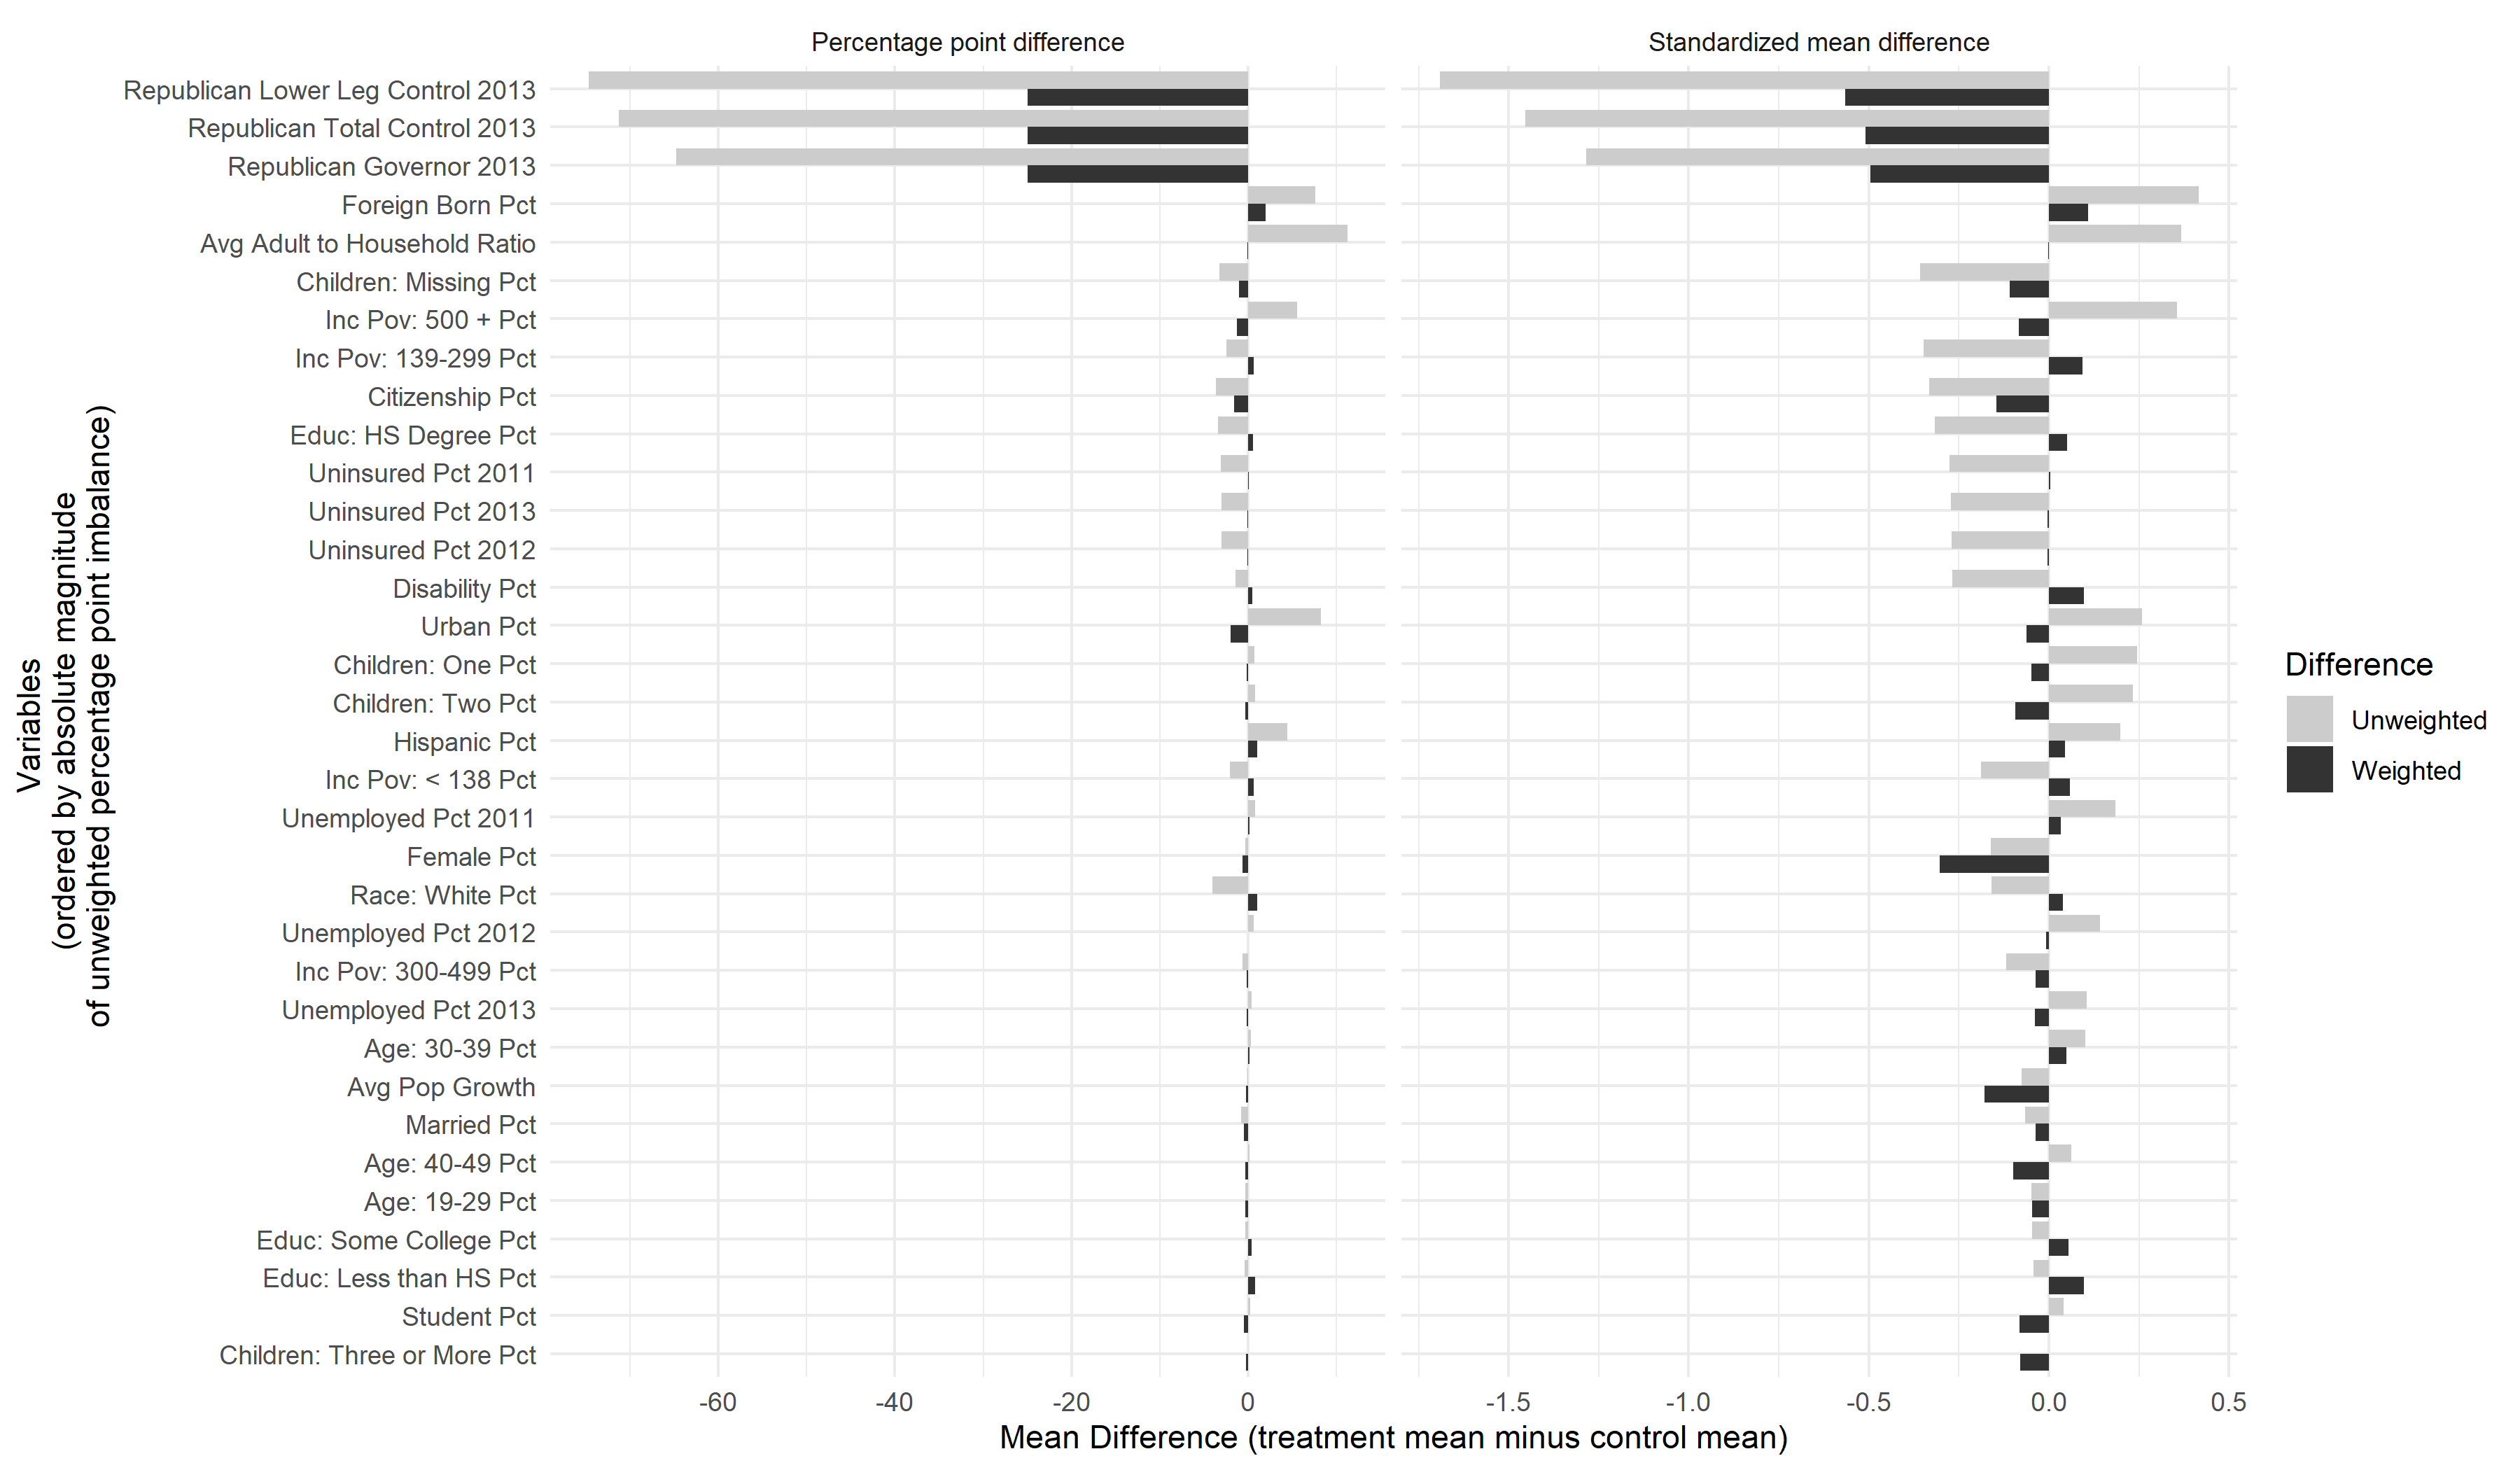
\includegraphics[scale=0.45]{01_Plots/balance-plot-all-etuc1.png}
\end{center}
\end{figure}

\begin{figure}[H]
\begin{center}
    \caption{H-SBW versus BC-HSBW versus SBW, weights summed by state, primary dataset}
    \label{fig:sbwvhsbw1}
    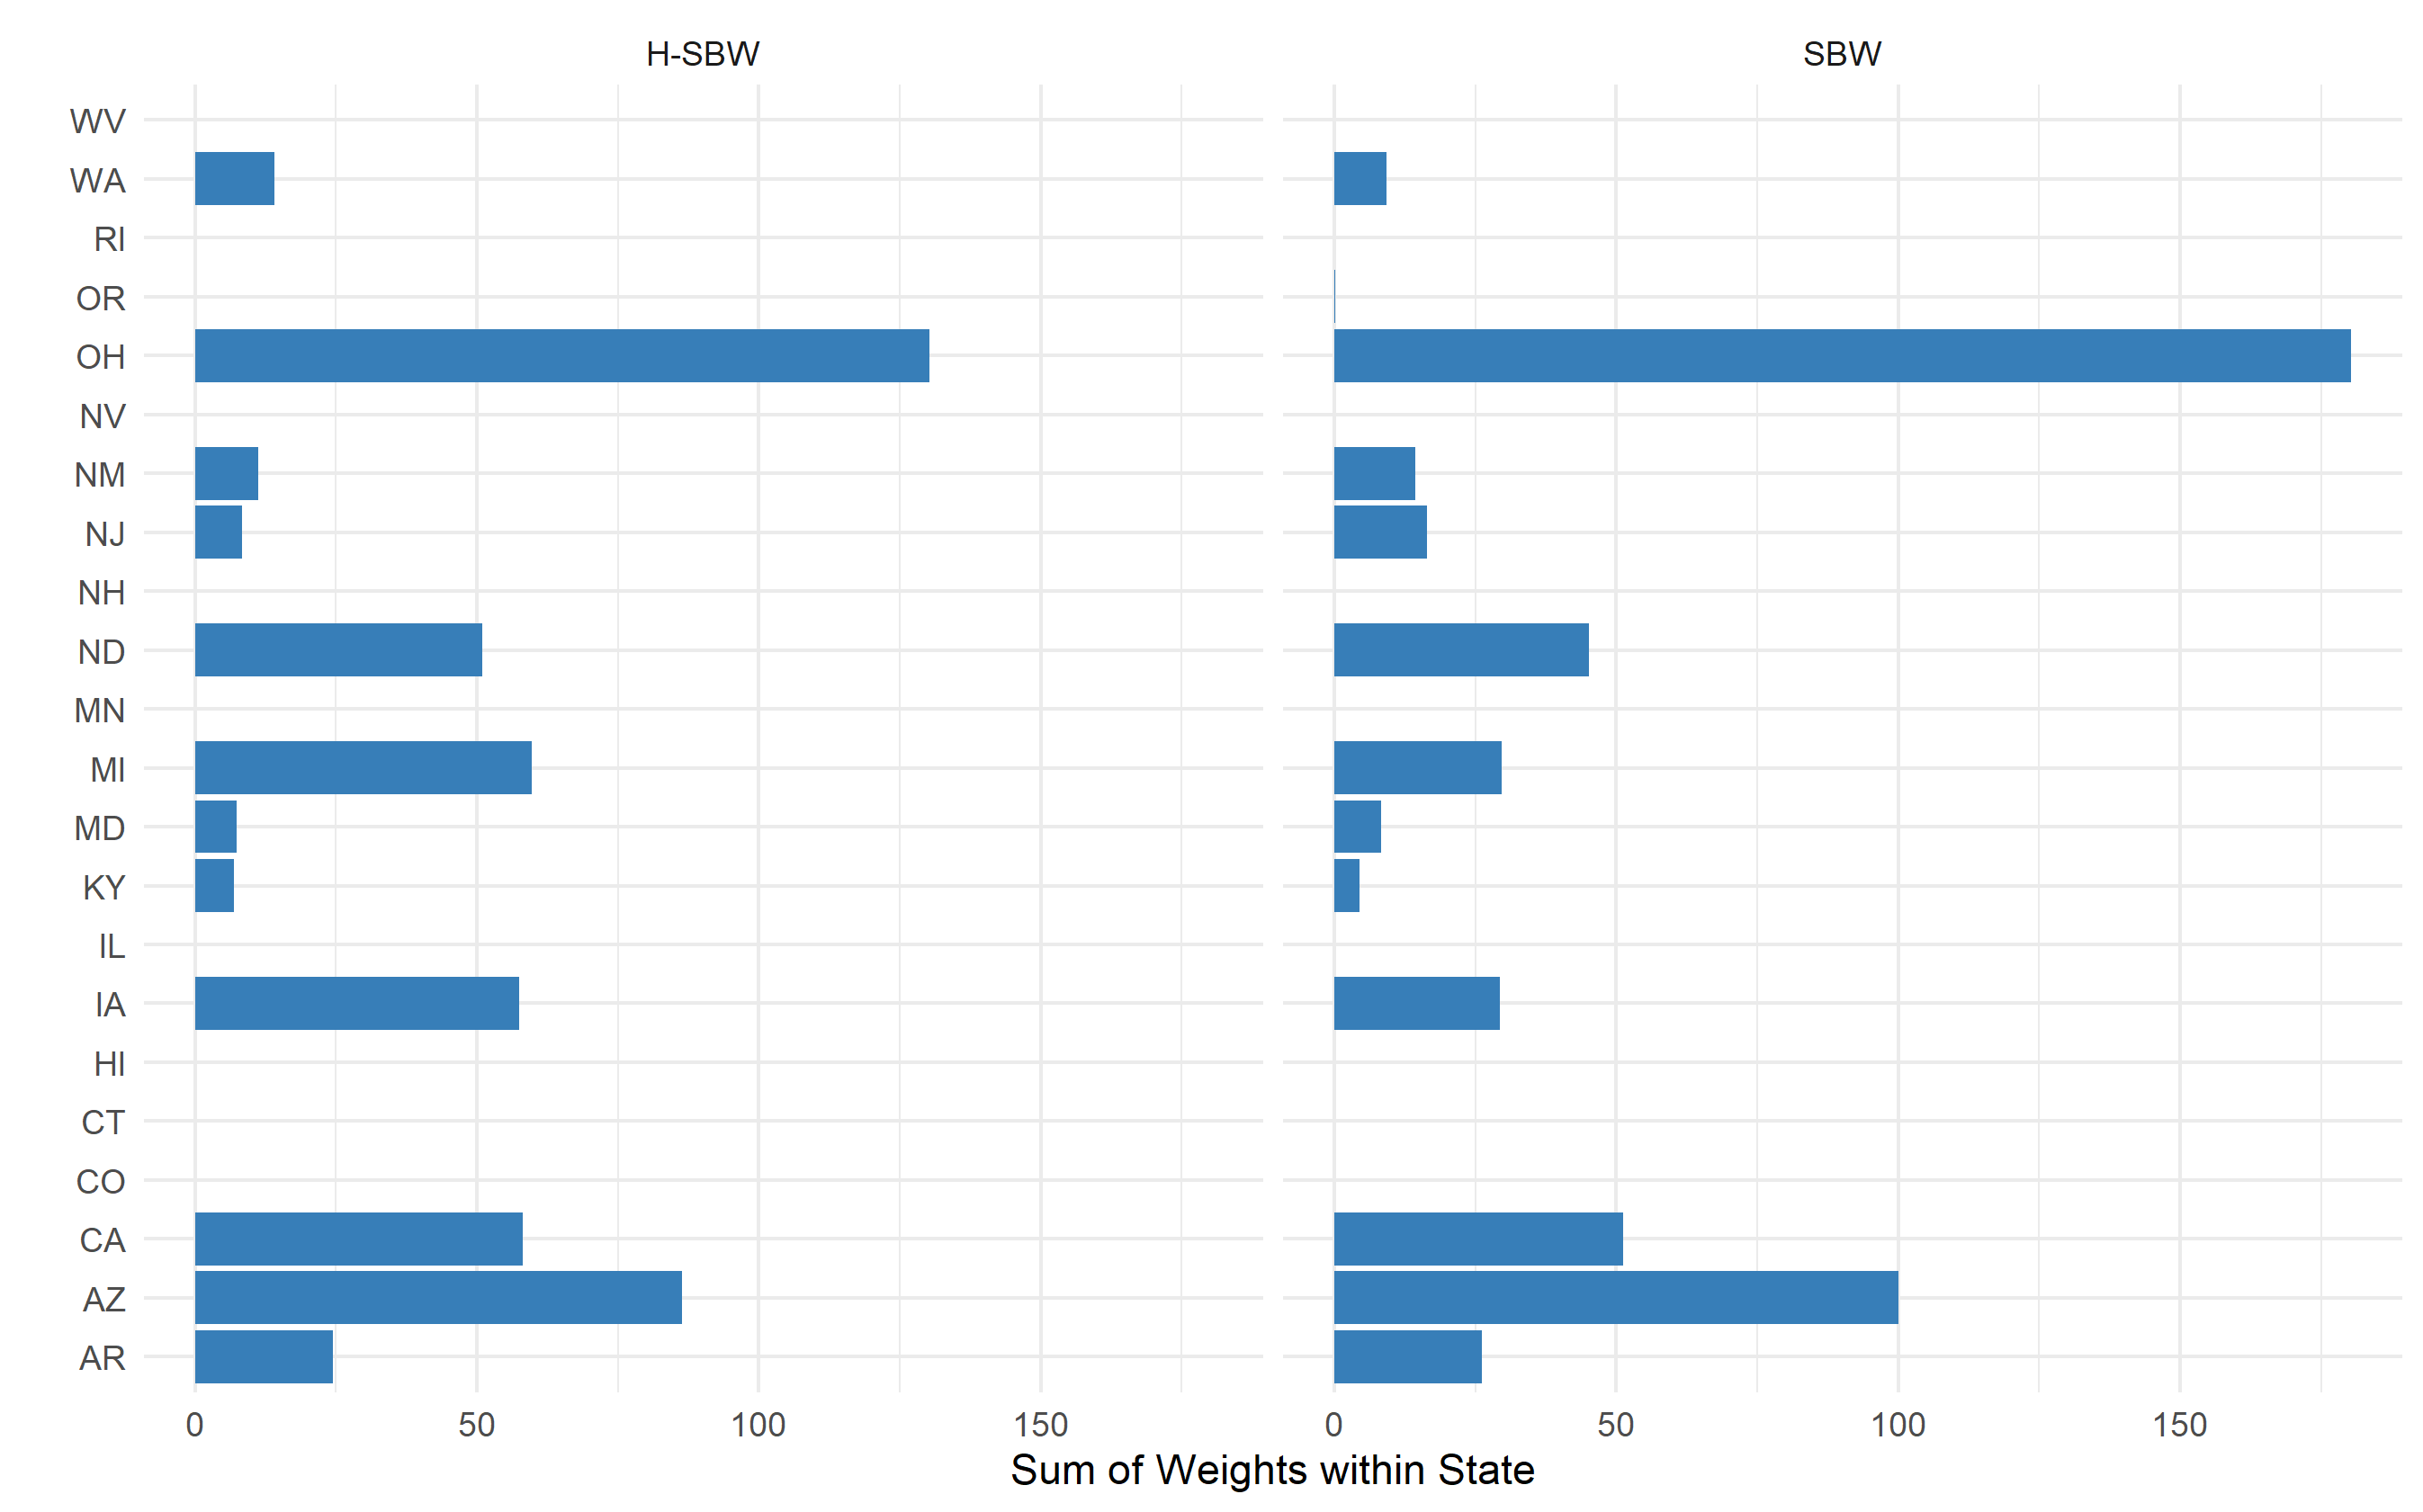
\includegraphics[scale=0.55]{01_Plots/weights-by-state-sbw-hsbw-c1.png}
\end{center}
\end{figure}

We then augment these weights using ridge-regression. Figure~\ref{fig:sbwvhsbw1} shows the total weights summed across states for three estimators: H-SBW, BC-HSBW, and SBW. For BC-HSBW we display the negative weights separately from the positive weights to highlight the extent of the extrapolation. This figure illustrates two key points: first, that H-SBW more evenly disperses the weights across states relative to SBW; second, that BC-HSBW extrapolates somewhat heavily in order to achieve the desired level of balance, particularly for CPUMAs in California (this is likely in part because California has the most CPUMAs of any state in the dataset).

We conclude by examining whether the H-SBW weights generated using the unadjusted data balance the adjusted covariates. While these metrics do not reflect the ``true'' imbalances, the comparison can provide some indication of whether the unadjusted weights are overfitting to noisy covariate measurements. Table~\ref{tab:balcomp} compares the imbalances among our pre-treatment outcomes using H-SBW weights generated on our unadjusted dataset applied to the adjusted (homogeneous) dataset. The ``Unweighted Difference'' column represents the raw difference in means, while the ``Weighted Difference'' column reflects the weighted difference that we calculate on the unadjusted dataset. The ``Homogeneous Diff'' column displays the weighted imbalance when applying the H-SBW weights to the dataset using the homogeneous adjustment, and similarly for ``Heterogeneous Diff.'' The weighted pre-treatment outcomes are approximately one percentage point lower than we desired in the two years prior to treatment using the heterogeneous adjustment, and -0.2 percentage points lower on average using the homogeneous adjustment. On the other hand, the naive difference suggests that the imbalance is only -0.05 percentage points. This result suggests that the unadjusted weights are overfitting to noisy covariates and may give an overly optimistic view of the covariate balance. Given the high degree of expected correlation between pre-treatment and post-treatment outcomes, we may expect the estimator of $\psi^1_0$ trained on the unadjusted data to have a negative bias.

v
\begin{table}[ht]
\caption{Balance comparison: weights estimated on unadjusted data applied to adjusted data}\label{tab:balcomp}
\begin{tabular}{lrrrr}
  \hline
Variables & Unweighted Diff & Weighted Difference & Homogeneous Diff & Heterogeneous Diff\\ 
  \hline
Uninsured Pct 2011 & -3.09 & -0.05 & -0.11 & 0.92 \\ 
  Uninsured Pct 2012 & -2.99 & -0.05 & -0.21 & -1.06 \\ 
  Uninsured Pct 2013 & -3.00 & -0.05 & -0.38 & -0.93 \\
   \hline
\end{tabular}
\end{table}

\subsubsection{Model validation}

We compare the performance of our models by repeating the covariate adjustments and calculating our procedure on 2009-2011 ACS data to predict 2012 outcomes, and similarly for 2010-2012 data to predict 2013 outcomes for the untreated states. We denote these outcomes $\psi^0_{0, t}$ for time-period $t$. Table~\ref{tab:pretxpred} displays these results, with the rows ordered by RMSE of the prediction errors. Table~\ref{tab:pretxpred} shows that the estimators trained on the covariate adjusted data have substantially better performance than the unadjusted data (``Sigma estimate'' = None). We also see that the estimators trained on the homogeneous adjustment outperform their counterparts on the heterogeneous adjustment. We therefore prioritize the results using the homogeneous adjustment. In these earlier years we find that SBW tends to have slightly lower RMSE than H-SBW, though the overall results are quite similar. Finally, these results show that estimators that extrapolate beyond the support of the data (the ridge-augmented versions ``BC-'') tend to perform worse. The worst performing estimators are the bias-corrected estimators trained on the unadjusted data.\footnote{In Appendix~\ref{app:allresults}, Table~\ref{tab:pretxpredfull} we also include the implied regression weights from OLS and GLS models, which exactly balance the observed covariates. When considering these estimators, the worst performing estimators are the OLS and GLS weights on the adjusted data, with OLS and GLS on the unadjusted data performing comparably to BC-SBW and BC-HSBW.} While this does not imply that these models will necessarily perform poorly when predicting $\psi^1_{0, T}$, it does suggest caution. We interpret this result as a function of our models being approximations: linearity may approximately hold on the support of the data where we have sufficient covariate overlap, but is more likely to lead us astray when extrapolating beyond the support of the data.

\begin{table}[ht]
\caption{Estimator
pre-treatment outcome prediction error (in \% pts)}\label{tab:pretxpred}
\begin{tabular}{llrrr}
  \hline
Sigma estimate & Estimator & 2011 error & 2012 error & RMSE \\ 
  \hline
Homogeneous & SBW & -0.18 & -0.22 & 0.20 \\ 
  Homogeneous & H-SBW & -0.24 & -0.21 & 0.23 \\ 
  Heterogeneous & SBW & -0.25 & -0.30 & 0.27 \\ 
  Heterogeneous & H-SBW & -0.32 & -0.39 & 0.36 \\ 
  Homogeneous & BC-SBW & -0.42 & -0.35 & 0.39 \\ 
  Heterogeneous & BC-SBW & -0.45 & -0.39 & 0.42 \\ 
  None & SBW & -0.50 & -0.61 & 0.56 \\ 
  None & H-SBW & -0.52 & -0.61 & 0.57 \\ 
  Homogeneous & BC-HSBW & -0.53 & -0.62 & 0.58 \\ 
  Heterogeneous & BC-HSBW & -0.53 & -0.72 & 0.63 \\ 
  None & BC-SBW & -0.82 & -0.93 & 0.88 \\ 
  None & BC-HSBW & -0.93 & -0.99 & 0.96 \\ 
   \hline
\end{tabular}
\end{table}

Our estimators also uniformly under-predict the true uninsurance rate. These errors range from between a fifth to a whole percentage point. This finding is not unexpected: intuitively, this is a form of regression-to-the-mean caused by overfitting our weights to noisy covariate measurements. More formally, we can think of the uninsurance rates in time period $t$ in in expansion and non-expansion regions as being drawn from separate distributions ($Y_{sct} \mid A_s$) with means $(\upsilon_1, \upsilon_0)$ where $\upsilon_1 < \upsilon_0$. For simplicity assume that $Y_{sc} = Y_{sct} = \alpha_1 + \beta_1Y_{sct-1} + \epsilon_{sct}$ where $\beta_1 > 0$. Applying our measurement error model applied to the pre-treatment outcomes ($J_{sct-1} = Y_{sct-1} + \nu_{sct-1}$) suggests that generating weights $\hat{\gamma}_{sc}$ that reweight $J_{sct}A_{sct}$ to $\upsilon_0$, $\sum_{A_{sc} = 1}\hat{\gamma}_{sc}\nu_{sct-1}$ is likely to be positive. Therefore the weights will not balance the true $Y_{sct-1}$ to $\upsilon_0$, but instead we should find that $\mathbb{E}[\sum_{A_{sc} = 1}Y_{sct-1}\hat{\gamma}_{sc}] \le \upsilon_0$. Under our modeling assumptions, this implies that we can expect a negative bias: $\mathbb{E}[\beta_1(\sum_{A_{sc} = 1}\hat{\gamma}_{sc}Y_{sct-1} - \upsilon_0)] \le 0$. \footnote{This phenomenon has also been discussed in the difference-in-differences and synthetic controls literature (see, e.g., \cite{daw2018matching}).} 
Our covariate adjustments are meant to eliminate this bias; however, in practice they only appear to reduce it (though the residual bias may also be a function of model misspecification). Assuming these errors reflect a negative bias that will also hold for our estimates of $\psi^1_0$, we may expect that the true treatment effect is closer to zero than our estimate. 
\subsection{Primary Results}

Using H-SBW we estimate an effect of -2.33 (-3.47, -1.19) percentage points. The SBW results are almost identical with -2.35 (-3.67, -1.03) percentage points. Compared to the unadjusted data we see very similar point estimates at -2.34 (-2.85, -1.82) percentage points for H-SBW and -2.39 (-2.95, -1.83) percentage points for SBW. We see that H-SBW reduces the confidence interval width relative to SBW on our primary dataset, though the lengths are nearly identical when excluding early expansion states. Using the adjusted covariate set also increases the width of the confidence intervals relative to the unadjusted data. This increase in the variance estimated is expected in part because the adjustment procedure generally reduces the variability in the data, as we saw in Table~\ref{tab:adjust1}, requiring that the variance of the weights to increase to achieve approximate balance. More generally this increase reflects the uncertainty due to the measurement error.

Adding the bias-correction decreases the absolute magnitude of the estimates: we estimate effects of -2.05 (-3.22, -0.87) percentage points for BC-HSBW and -2.07 (-3.07, -1.06) percentage points for BC-SBW. In contrast to our validation tests, where the bias-corrected estimators tended to predict lower uninsurance rates than the other estimators, here the bias-corrected estimators predict higher uninsurance rates. Table~\ref{tab:mainresults} presents all of our primary estimates in the ``Estimate (95\% CI)'' column. All adjusted estimates were closer to zero than the unadjusted estimates, though the point estimates from the SBW and H-SBW were estimators were virtually identical. The estimates calculated using the heterogeneous adjustment were all closer to zero than the unadjusted estimates (results are available in Appendix~\ref{app:allresults}).

\begin{table}[ht]
\caption{Primary results}\label{tab:mainresults}
\begin{tabular}{lllc}
  \hline
Weight type & Adjustment & Estimate (95\% CI) & Estimate (95\% CI) (Early excluded) \\ 
  \hline
H-SBW & Homogeneous & -2.33 (-3.47, -1.19) & -2.09 (-3.15, -1.03) \\ 
  H-SBW & None & -2.34 (-2.85, -1.82) & -2.28 (-2.82, -1.74) \\ 
  BC-HSBW & Homogeneous & -2.05 (-3.22, -0.87) & -1.94 (-3.17, -0.72) \\ 
  BC-HSBW & None & -2.22 (-2.87, -1.56) & -2.22 (-3.07, -1.38) \\ 
  SBW & Homogeneous & -2.35 (-3.67, -1.03) & -2.05 (-3.10, -1.00) \\ 
  SBW & None & -2.39 (-2.95, -1.83) & -2.21 (-2.71, -1.72) \\ 
  BC-SBW & Homogeneous & -2.07 (-3.07, -1.06) & -1.99 (-3.22, -0.77) \\ 
  BC-SBW & None & -2.19 (-2.9, -1.49) & -2.23 (-3.05, -1.40) \\ 
   \hline
\end{tabular}
\end{table}

We consider the sensitivity of our analysis with respect to no anticipatory treatment effects and excluding the early expansion states (California, Connecticut, Minnesota, New Jersey, and Washington), and re-run our analyses. The column ``Early excluded estimate (95\% CI)'' in Table~\ref{tab:mainresults} above reflects these results. Our point estimates are similar to our primary analysis, though the numbers move slightly closer to zero. We also see that the difference between the estimates on the adjusted and unadjusted data is slightly larger: -2.28 (-2.82, -1.74) percentage points for H-SBW on the unadjusted dataset and -2.09 (-3.15, -1.03) on the adjusted data. We again find that the bias-correction moves the point estimates again closer to zero. Overall our primary results are relatively robust to the exclusion of these states. Additional diagnostics and results are available in Appendix~\ref{app:weightdiagnostic}.

Lastly, we examine the robustness of our point estimates to the removal of individual states (these are the same point estimates used to calculate our confidence intervals). Removing Ohio moved our point estimates farther from zero while removing North Dakota, Kentucky, or California moved our estimates closer to zero. Appendix~\ref{app:allresults}, Figure~\ref{fig:loostateplot} displays a heatmap showing how the estimates change for each estimator when removing each state.

\section{Discussion}

We divide our discussion into two sections: methodological and policy considerations and limitations. We begin with the former.

\subsection{Methodological considerations and limitations}

We make multiple contributions to the literature on balancing weights. First, our estimation procedure accounts for mean-zero random noise in our covariates that is uncorrelated with the outcome errors. We modify the constraint set to balance on a linear approximation to the true covariate values, applying the idea of regression calibration from the measurement error literature (\cite{gleser1992importance}) to the context of balancing weights. Our application illustrates the benefits of this procedure: using observed (pre-treatment) outcomes generated by an unknown data generating mechanism, Table~\ref{tab:pretxpred} demonstrates that our proposed approach substantially improves our predictive ability relative to existing approaches. When applying this approach to estimate our causal effect, we find that the naive estimators are larger in absolute magnitude than the adjusted estimates. This finding is consistent with our worries about overfitting to noisy covariate measurements and subsequent regression-to-the-mean.\footnote{See also \cite{daw2018matching}, who discuss this phenomenon in more detail in the context of difference-in-differences designs.}

This approach has at least three potential limitations: first, it requires access to auxillary data with which to estimate the measurement error covariance matrix $\Sigma_{\nu}$. Many applications may not have access to such information. Even without such information, $\Sigma_{\nu}$ could also be considered a sensitivity parameter to evaluate the robustness of results to measurement error (see, e.g., \cite{huque2014impact}, \cite{illenberger2020impact}). Second, from a theoretic perspective, strong distributional assumptions on the covariates are required to consistently estimate $\psi_0^1$ using convex balancing weights. This in contrast to \cite{gleser1992importance}, who finds that the OLS estimates are consistent with only very weak distributional assumptions on the data.\footnote{We show these findings more formally in the context of balancing weights in Appendix~\ref{app:AsecIII}.} We speculate this tradeoff is often worth it: by preventing extrapolation, SBW and H-SBW estimates are also less sensitive to assumptions on the outcome model, which is often the more costly assumption. Our model validation results support this for our application, as we find that the standard regression calibration adjustment using OLS and GLS actually performs by far the worst out of any methods we consider, including naive regression on the noisy covariate measurements (see Table~\ref{tab:pretxpredfull} in Appendix~\ref{app:allresults}). In contrast, our proposed method performs the best.

A final concern is that this procedure may be sub-optimal with respect to the mean-square error of our estimator. In particular, the bias induced by the measurement error decreases with square root of the sample size used to calculate each CPUMA's covariate values, the minimum of which were over three hundred. Meanwhile, the variance of our counterfactual estimate should decrease with the square root of the number of treated states. From a theoretic perspective, the variance is of a larger order than the bias, so perhaps the bias from measurement error should not be a first-order concern. Other studies have proposed tests of whether the measurement error corrections are ``worth it'' though we do not do so here (see, e.g., \cite{gleser1992importance}). Even so, our simulation study shows that confidence interval coverage can still fall below nominal rates when using the mismeasured covariates even in regimes when the measurement error is small relative to the variability in the outcome model. In our application we find that our point estimates are quite similar either way, but that confidence interval widths increase substantively, perhaps reflecting a more accurate estimate of the uncertainty.

Our second contribution is to introduce the H-SBW objective. This objective can improve upon the SBW objective assuming that the errors in the outcome model are homoskedastic with positive equi-correlation $\rho$ within some groupings of the units. Assuming we observe the true covariates, we show that H-SBW produces a lower variance estimator by more evenly dispersing weights across groups. While other studies have considered settings with hierarchical data (see, e.g., \cite{keele2020hospital}), we are the first study we are aware of to propose modifying the objective to reduce the variability in the subsequent estimates.

This procedure has at least three potential drawbacks: first, we make a very specific assumption on the covariance structure of the error terms that is useful for application. For other applications one could follow our approach and assume a different covariance structure $\Omega$ to generate weights that minimize the criterion $f(\gamma) = \gamma^T\Omega\gamma$. A second concern is that given our assumed covariance structure, we require specifying the parameter $\rho$ in advance. In our simulation study in Appendix~\ref{app:simstudy}, we find that even when choosing a sub-optimal $\rho$, the H-SBW estimator often has lower variance than SBW in the presence of state-level random effects. Our simulations consider the common setting where we have a relatively small number of groups ($m = 25$). We also find that when using SBW, the leave-one-state-out jackknife variance estimates have slightly lower than nominal coverage rates. We speculate that this may be because the weights are not sufficiently dispersed across enough states for the asymptotic approximation of the variance estimation procedure to hold. Supporting this hypothesis, we find that even $\rho$ is incorrect, H-SBW coverage rates improve over those for SBW. Regardless, identifying a data-driven approach to choose this tuning parameter (or perhaps for the covariance structure in general) could be a useful future contribution.

A final limitation of H-SBW is that in the context of measurement error, even if the covariates are Gaussian, if they are dependent using H-SBW with the simple regression-calibration adjustment may lead to subsequent bias in the effect estimates (see Appendix~\ref{app:AsecIII}). On the other hand, our simulations in Appendix~\ref{app:simstudy} suggest that this dependence does not bias the SBW estimates. This suggests that SBW may be more useful in the context of measurement error than H-SBW. Even so, we find in our simulation study that this bias is often small, and H-SBW still may have MSE improvements relative to SBW. Moreover, for our application our SBW and H-SBW estimates are quite comparable. We caution that the bias also increases with $\rho$: therefore, if using H-SBW with the simple regression-calibration adjustment, one may wish to keep $\rho$ small. If this remains unsatisfactory, we show in Appendix~\ref{app:AsecIII} that we can modify the regression-calibration procedure to remove this bias asymptotically, though we do not do this for this application.

\subsection{Policy considerations and limitations}

We estimate that had states that did not expand Medicaid in 2014 instead expanded their programs, they would have seen a -2.33 (-3.47, -1.19) percentage point change in the adult uninsurance rate. Existing estimates place the ETT between -3 and -6 percentage points. These estimates vary depending on the targeted sub-population of interest, the data used, the level of modeling (individuals or regions), and the modeling approach (see, e.g., \cite{courtemanche2017early}, \cite{kaestner2017effects}, \cite{frean2017premium}). Our estimate of the ETC are closer to zero than these estimates. When we attempt to estimate the ETT using our approach, the resulting estimates have high uncertainty due to limited covariate overlap.\footnote{In particular, there were no states entirely controlled by Democrats that did not expand Medicaid. Even allowing for large imbalances in the governance covariates, our standard error estimates were approximately three percentage points and our confidence intervals all contained zero. When estimating a simple difference-in-differences model on the unadjusted dataset we estimate that the ETT is -2.05 (-3.12, -0.97), where the standard errors account for clustering at the state level.} The differences may reflect different modeling strategies and data, or it may suggest that the ETC is smaller in absolute magnitude than the ETT.

We ultimately make no formal statistical claims about these differences, however, we emphasize the importance of caution when using estimates of the ETT to make inferences about the ETC. Because almost every outcome of interest is mediated through increasing the number of insured individuals, if the ETC is in fact different than the ETT, then projecting findings from an estimate of the ETT to the ETC may lead to inaccurate inferences. For example, \cite{miller2019medicaid} study the effect of Medicaid expansion on mortality. Using their estimate of the ETT they project that had all states expanded Medicaid, 15,600 deaths would have been avoided during their study's time-period. If we believe that this number increases monotonically with the number of uninsured individuals, this estimate may be an overestimate if the ETC is less than the ETT, or an underestimate if the ETC is greater than the ETT. Directly estimating the ETC can help us better model policy relevant downstream effects mediated through decreasing the uninsurance rate. 

Our estimate is not without limitations. Specifically, our analysis requires many strong modeling assumptions. In particular, we require SUTVA, no anticipatory treatment effects, no unmeasured confounding conditional on the true covariates, and several parametric assumptions regarding the outcome and measurement error models. We were able to address some concerns about possible violations of these assumptions. For example, our results were qualitatively similar whether we excluded possible ``early expansion states,'' or used different weighting strategies (including relaxing the positivity restrictions and changing the tuning parameter $\rho$). However, we do not attempt to address concerns about the impact of spillovers across regions. And while we believe that no unmeasured confounding is reasonable for this problem, we did not conduct a sensitivity analysis (see, e.g., \cite{bonvini2021sensitivity}) with respect to this assumption. 

Medicaid expansion remains an ongoing policy debate in the United States. Following the passage of the American Rescue Plan, state legislatures in Wyoming, Alabama, and North Carolina are reportedly considering expanding their programs. Our study estimates the effect of Medicaid expansion on adult uninsurance rates; however, this effect is only interesting because Medicaid enrollment is not automatic for eligible individuals. Different state policies may therefore make it easier or harder to enroll in Medicaid. If the goal of Medicaid expansion is to increase insurance access for low-income adults, state policy-makers also may wish to make it easier to enroll in Medicaid. 

\section{Conclusion}

We predict the change in the non-elderly adult uninsurance rate in 2014 among states that did not expand Medicaid as if they had expanded Medicaid. We use survey data aggregated to the CPUMA-level to estimate this effect. The resulting dataset has both measurement error in the covariates that may bias standard estimation approaches, and a hierarchical structure that may worsen the efficiency of these same approaches. We therefore propose an estimation procedure that accounts for these problems. We demonstrate that our method improves on existing approaches when predicting observed outcomes from an unknown data generating mechanism. Applying our method to our problem, we then estimate that states that did not expand Medicaid in 2014 would have seen a -2.33 (-3.47, -1.19) percentage point change in their adult uninsurance rates had they done so. This is the first study we are aware of that directly estimates the treatment effect on the controls with respect to Medicaid expansion. From a methodological perspective, we demonstrate the value of our proposed method relative to existing ones. From a policy-analysis perspective, we emphasize the importance of directly estimating the relevant causal quantity of interest. More generally if the goal of Medicaid expansion is to increase access to insurance for low-income adults, state and federal policy-makers may wish to consider policies that make Medicaid enrollment easier if not automatic.

\section*{Acknowledgements}

The authors gratefully acknowledge invaluable advice and comments from Zachary Branson, Riccardo Fogliato, Edward Kennedy, Brian Kovak, Akshaya Jha, Lowell Taylor, and Jose Zubizaretta.

\begin{supplement}
Analysis programs and supporting materials are available online at \url{github.com /mrubinst757/medicaid-expansion}. Proofs and additional results are available in the Appendix.
\end{supplement}

\bibliographystyle{imsart-nameyear} % Style BST file
\bibliography{research.bib}       % Bibliography file (usually '*.bib')

\clearpage

\appendix

\section{Proofs}\label{ssec:proof}

We divide our proofs into three sections: the first two consist of propositions and the third contains the proofs of the propositions. In the first section our propositions pertain to the performance of SBW under the classical measurement error model. Our key results are that the bias of the SBW estimator is equivalent to the bias of the OLS estimator and that regression-calibration techniques can be used in this setting to obtain consistent estimators. However, these results assume that the data are gaussian. We also show that if the data are not gaussian, the OLS estimator using regression-calibration remains consistent, while the SBW estimator may be biased. In our second section we consider the properties of the H-SBW objective when the true covariates $X$ are observed. We show that if our assumed correlation structure for the outcome errors is correct, H-SBW produces the minimum conditional-on-X variance estimator within the constraint set. We also show how a generalized form of H-SBW weights relate to the implied regression weights from Generalized Least Squares (GLS). We conclude by showing that H-SBW may yield biased estimates if we do not correctly model the dependence structure of the data. Section~\ref{app:AsecIII} contains all of the proofs.

\subsection{SBW and classical measurement error}\label{app:AsecI}

We begin by showing six results regarding the bias of the OLS and SBW estimators under the classical errors-in-variables model. First, we show that without adjustment for errors-in-covariates, the bias of the SBW estimator that sets $\delta = 0$ (i.e. reweights the treated units to exactly balance the control units) is equal to the bias of the OLS estimator. Second, we show that if the observed covariate values for the treated data can be replaced by their conditional expectations $\tilde{X}$ given the noisy observations, then the SBW estimator will be unbiased and consistent. Third, we consider the case where $\tilde{X}$ must be estimated, and show that the SBW estimator is consistent if we replace $\tilde{X}$ by a consistent estimate $\hat{X}$. Finally, we remove the assumption that $X$ is gaussian, and show that while the OLS estimator remains unbiased under weaker assumptions, the SBW estimator does not, and we show a general expression for the asymptotic bias. We take the perspective throughout that $X$ is random among the treated units but fixed for the control units.

We assume that equations (\ref{eqn:unconfoundedness}) - (\ref{eqn:Xgaussian}) hold. For simplicity, we additionally assume that
\begin{equation}\label{eqn:simplifications}
\epsilon_{sc} = 0, \quad \varepsilon_s = 0,\quad \xi_{sc} = 0,\quad  \Sigma_{\nu,sc} = \Sigma_\nu, \qquad \forall s,c
\end{equation}
noting that $\xi_{sc}=0$ implies $J_{sc} = Y_{sc}$. The covariate observations of the treated units can then be seen to be i.i.d., with covariance matrix
\[ \Sigma_{W|1} = \Sigma_{X|1} + \Sigma_\nu,\]
and the conditional expectation of $X_{sc}$ given $W_{sc}$ for the treated units can be seen to equal
\[ \tilde{X}_{sc} = v_1 + \kappa^T (W_{sc} - v_1), \qquad \forall sc: A_{sc}=1,\]
where
\[ \kappa = (\Sigma_{X|1} + \Sigma_{\nu})^{-1} \Sigma_{X|1}.\]
To ease notation, we abbreviate $\Sigma_X = \Sigma_{X \mid 1}$ and similarly $ \Sigma_W = \Sigma_{W \mid 1}$. 

In Propositions \ref{cl8}, \ref{cl9}, and part of Proposition \ref{cl1}, we will remove the Gaussian covariate assumption given by \eqref{eqn:Xgaussian}. In its place, we will instead consider the weaker assumption that the empirical covariance of $X$ has a limit $S_X$,

\begin{equation}\label{eqn:limitX}
 \frac{1}{n_1} \sum_{A_{sc}=1} (X_{sc} - \bar{X}_1)(X_{sc} - \bar{X}_1)^T \rightarrow^p S_X,
\end{equation}
which implies a similar limit $S_W$ for the noisy observations $W$,

\begin{equation}\label{eqn:limitW}
 \frac{1}{n_1} \sum_{A_{sc}=1} (W_{sc} - \bar{W}_1)(W_{sc} - \bar{W}_1)^T \rightarrow^p S_W = S_X + \Sigma_{\nu},
\end{equation}
where we have used the independence of the noise terms $\nu_{sc}$, and similarly that 
\begin{equation}\label{eqn:limitWY}
 \frac{1}{n_1} \sum_{A_{sc}=1} (W_{sc} - \bar{W}_1)(Y_{sc} - \bar{Y}_1)^T \rightarrow^p S_X \beta_1,
\end{equation}
where we have additionally used the linear model for $Y_{sc}$ given by \eqref{eqn:linmod}.

We first consider estimation without adjustment for errors in covariates. 
Proposition \ref{cl1} states that the unadjusted OLS and SBW estimators have equal bias, with the bias of the OLS estimator remaining unchanged if the gaussian assumption of \eqref{eqn:gaussiannoise} is removed.

\begin{proposition}\label{cl1}
Let (\ref{eqn:unconfoundedness}) - (\ref{eqn:Xgaussian}) and (\ref{eqn:simplifications}) hold.
Let $(\hat{\alpha}, \hat{\beta})$ denote the unadjusted OLS estimator of $(\alpha_1, \beta_1)$, 
\begin{equation}\label{eqn:prop1.beta}
(\hat{\alpha}, \hat{\beta}) = \arg \min_{\alpha, \beta} \sum_{sc:A_{sc}=1} (Y_{sc} - \alpha -  W_{sc}^T\beta)^2,
\end{equation}
which induces the OLS estimator of $\psi_0^1$ given by

\begin{align*}
\hat{\psi}^{1,\textup{ols}}_0 = \bar{Y}_1 + (\bar{W}_0 - \bar{W}_1)^T\hat{\beta}_1.
\end{align*}
%
Let ${\gamma}$ denote the unadjusted SBW weights under exact balance, found by solving \eqref{eqn:SBWobjective} with constraint set $\Gamma( W_{A=1}, \bar{W}_0, 0)$, which induces the SBW estimator of $\psi_0^1$ given by

\begin{align*}
\hat{\psi}^{1,\textup{sbw}}_0 = \sum_{sc: A_{sc} = 1} {\gamma}_{sc} Y_{sc}.
\end{align*}
%
Then the estimators $\hat{\psi}^{1, \textup{ols}}_0$ and $\hat{\psi}^{1, \textup{sbw}}_0$ have equal bias, satisfying

\begin{align*}
\mathbb{E}[\hat{\psi}_0^{1,\textup{ols}}] &= \mathbb{E}[\hat{\psi}^{1, \textup{sbw}}_0]  = \psi_0^1 + (\bar{X}_0 - \upsilon_1)^T(\mathbf{\kappa} - I_q)\beta.
\end{align*}
Additionally, the bias of $\hat{\psi}_0^{1,\textup{ols}}$ is asymptotically unchanged if the gaussian covariate assumption given by \eqref{eqn:Xgaussian} is replaced by \eqref{eqn:limitX}.
\end{proposition}

To study the SBW estimator with covariate adjustment, we first consider an idealized version where $\Sigma_X$ and $\Sigma_\nu$ are known, so that $\tilde{X}_{A=1}$ is also known. Proposition \ref{cl2} shows that the resulting estimate of $\psi_0^1$ is unbiased if $\delta = 0$.

\begin{proposition}\label{cl2}
Let (\ref{eqn:unconfoundedness}) - (\ref{eqn:Xgaussian}) and (\ref{eqn:simplifications}) hold. Let $\tilde{X}_{A=1}$ equal the conditional expectation of $X_{A=1}$ given $W$,

\[ \tilde{X}_{sc} = \upsilon_1 + \kappa^T (W_{sc} - \upsilon_1), \qquad \forall sc: A_{sc} = 1,\] let $\gamma^*$ be the solution to the SBW objective defined over the constraint set $\Gamma(\tilde{X}_{A=1}, \bar{X}_0, 0)$, and let $\hat{\psi}^{1, \textup{ideal}}_0$ be the SBW estimator $\sum_{sc: A_{sc} = 1}\gamma^\star_{sc}Y_{sc}$. This estimator is unbiased for $\psi_0^1$.
\end{proposition}



Proposition \ref{prop:variance_rate} shows that the variance of this idealized SBW estimator goes to zero, implying consistency. 
\begin{proposition}\label{prop:variance_rate}
Let (\ref{eqn:unconfoundedness}) - (\ref{eqn:Xgaussian}) and (\ref{eqn:simplifications}) hold, and let $\gamma^*$ and $\hat{\psi}_0^{1, \textup{ideal}}$ be defined as in Proposition \ref{cl2}. Then the conditional variance of the estimation error is given by

\begin{align*}
\operatorname{Var}\left( \hat{\psi}_0^{1, \textup{ideal}} - \psi_0^1| W\right)  = \|\gamma^*\|^2 \cdot \beta_1^T(\Sigma_{X} - \Sigma_{X}\Sigma_{W}^{-1}\Sigma_{X})\beta_1, 
\end{align*}
with $\operatorname{Var}\left( \hat{\psi}_0^{1, \textup{ideal}} - \psi_0^1| W\right)$ and $\operatorname{Var}(\hat{\psi}_0^{1,\textup{ideal}})$ both behaving as $O_P(n_1^{-1})$ as $n_1 \rightarrow \infty$.
\end{proposition}

In practice, the idealized SBW estimator considered in Propositions \ref{cl2} and \ref{prop:variance_rate} cannot be used, as $\Sigma_X$ and $\Sigma_{\nu}$ are not known, but instead must be estimated from auxilliary data. Proposition \ref{cl3} states that if these estimates are consistent, then the resulting adjusted SBW estimator for $\psi_0^1$ is also consistent if $\delta = 0$.

\begin{proposition}\label{cl3}
Let (\ref{eqn:unconfoundedness}) - (\ref{eqn:Xgaussian}) and (\ref{eqn:simplifications}) hold. Given estimates $\hat{\Sigma}_X$ and $\hat{\Sigma}_\nu$ that are consistent for $\Sigma_X$ and $\Sigma_\nu$, let $\hat{X}_{A=1}$ be given by 
\[ \hat{X}_{sc} = \bar{W}_1 + \hat{\kappa}^T(W_{sc} - \bar{W}_1), \]
where $\hat{\kappa} = (\hat{\Sigma}_X + \hat{\Sigma}_{\nu})^{-1} \hat{\Sigma}_X$. Let $\hat{\gamma}$ be the weights that solve the SBW objective over the constraint set $\Gamma(\hat{X}_{A=1}, \bar{W}_0, 0)$, and let $\hat{\psi}^{1, \textup{adjusted}}_0 = \sum_{sc: A_{sc} = 1} \hat{\gamma}_{sc} Y_{sc}$ be the corresponding SBW estimator. This estimator is consistent for $\psi_0^1$ as $n_1 \to \infty$.
\end{proposition}

In (\ref{eqn:jackknife}) we propose a leave-one-state-out jackknife estimate of variance. Following \cite{efron1981jackknife}, this estimate can be decomposed a conservatively biased estimate of the variance of $\hat{\psi}_0^{1, \textup{adjusted}}$ given a sample size of $(m_1-1)$ treated states, plus a heuristic adjustment to go from sample size $(m_1-1)$ to sample size $m_1$, when treating the observations of the control states as fixed.

\begin{proposition}\label{prop:jackknife}
Let (\ref{eqn:unconfoundedness}) - (\ref{eqn:gaussiannoise}) hold, and additionally assume that $p_s$, the number of CPUMAs, is i.i.d. in the treated states. Let $\hat{\operatorname{Var}}(\hat{\psi}_0^{1, \textup{adjusted}}) = \frac{m_1-1}{m_1} \cdot \tilde{\operatorname{Var}}(\hat{\psi}_0^{1, \textup{adjusted}})$, where

\begin{equation} \label{eqn:prop.jackknife}
\tilde{\operatorname{Var}}(\hat{\psi}_0^{1, \textup{adjusted}}) = \sum_{s:A_{s}=1} (S_{(s)} - S_{(\cdot)})^2,
\end{equation}
with $S_{(s)}$ and $S_{(\cdot)}$ as defined for \eqref{eqn:jackknife}. Then $\tilde{\operatorname{Var}}$ is conservatively biased for the variance of the leave-one-state-out estimate,

\[ \mathbb{E}\left[ \tilde{\operatorname{Var}}(\hat{\psi}_0^{1, \textup{adjusted}})\right] \geq \operatorname{Var}(S_{(1)} | \bar{W}_0),\]
where $S_{(1)}$ can be seen to equal the estimator $\hat{\psi}_0^{1,\textup{adjusted}}$ under a sample size of $(m_1-1)$ treated states.

\end{proposition}

As the gaussian covariate assumption given by \eqref{eqn:Xgaussian} is strong, it would be desirable if the adjusted OLS or SBW estimators were consistent even for non-gaussian $X$. Proposition \ref{cl8} shows under mild assumptions that this is in fact true when running OLS on the adjusted covariates. 

\begin{proposition}\label{cl8}
Let (\ref{eqn:unconfoundedness}) - (\ref{eqn:gaussiannoise}), and (\ref{eqn:simplifications})- (\ref{eqn:limitX}) hold, with $S_X$ invertible. Let $(\check{\alpha}, \check{\beta})$ denote the adjusted OLS estimates of $(\alpha_1, \beta_1)$, solving

\[ \min_{\alpha,\beta} \sum_{A_{sc}=1} (Y_{sc} - \alpha - \check{X}_{sc}^T \beta)^2, \]
where $\check{X}_{sc} = \bar{W}_1 + \check{\kappa}^T(W_{sc} - \bar{W}_1)$ with $\check{\kappa} = (S_X + \Sigma_\nu)^{-1}S_X$. Then the adjusted OLS estimator of $\psi_0^1$ given by
\[ \bar{Y}_1 - (\bar{W}_0 - \bar{W}_1)^T \check{\beta},\]
remains consistent if the gaussian assumption given by \eqref{eqn:gaussiannoise} is removed.
\end{proposition}

However, the same does not hold for the adjusted SBW estimator. Proposition \ref{cl9} gives an expression for its bias when the covariates are non-gaussian. 

\begin{proposition}\label{cl9}
Let the assumptions of Proposition \ref{cl8} hold. Let $\check{\gamma}$ solve the SBW objective over the constraint set $\Gamma(\check{X}_{A=1}, \bar{W}_0, 0)$ where $\check{X}_{A=1}$ and $\check{\kappa}$ are defined as in Proposition \ref{cl8}. Let $Q$ denote the set of indices where $\check{\gamma}$ is non-zero,

\[ Q = \{sc: \check{\gamma}_{sc} > 0\},\]
with cardinality $n_Q = |Q|$, and let $\bar{W}_Q$ and $S_{W_Q}$ denote the empirical mean and covariance of $\{W_{sc}:sc \in Q\}$,

\[ \bar{W}_Q = \frac{1}{n_Q}\sum_{sc \in Q} W_{sc},\qquad S_{W_Q} = \frac{1}{n_Q} \sum_{sc \in Q} (W_{sc} - \bar{W}_Q)(W_{sc} - \bar{W}_Q)^T,\]
with $\bar{X}_Q$ the analogous empirical mean of $\{X_{sc}:sc \in Q\}$ and $S_{XW_Q}$ the empirical cross covariance,
\[ S_{XW_Q} = \frac{1}{n_Q} \sum_{sc \in Q} (X_{sc} - \bar{X}_Q)(W_{sc} - \bar{W}_Q)^T.\]
Then if the gaussian assumption given by \eqref{eqn:gaussiannoise} is removed, the adjusted SBW estimator for $\psi_0^1$ given by 

\[\sum_{A_{sc}=1} Y_{sc} \check{\gamma}_{sc},\]
may be biased for $\psi_0^1$, with estimation error given by 

\begin{align} 
\nonumber \sum_{A_{sc}=1} Y_{sc} \check{\gamma}_{sc} - \psi_0^1 & = \beta_1^T\Big[(S_{XW_Q}S_{W_Q}^{-1}S_WS_X^{-1} - I)\bar{X}_0  + (\bar{X}_Q - S_{XW_Q}S_{W_Q}^{-1} S_W S_X^{-1} \bar{X}_1) \\
& \hskip1cm {} - S_{XW_Q}S_{W_Q}^{-1}(\bar{X}_Q - \bar{X}_1)\Big](1 + o_P(1)),  \label{eqn:cl9.error}
\end{align}
which need not converge to zero unless $\bar{X}_Q \to \bar{X}_1$, $S_{XW_Q} \to S_X$, and $S_{W_Q} \to S_W$.
\end{proposition}

Proposition \ref{cl7} shows that if the conditional expectations can be computed for the treated units (which may be computationally difficult or require strong modeling assumptions if the data is non-gaussian, or if dependencies exist between CPUMAs), then SBW yields unbiased estimates. 

\begin{proposition}\label{cl7}
    Let equations (\ref{eqn:unconfoundedness})-(\ref{eqn:linmod}) hold. Let $\tilde{X}^*$ denote the conditional expectation,
    \[\tilde{X}^*_{sc} = \mathbb{E}[X_{sc} | W, A_{sc}=1],\]
    let weights $\tilde{\gamma}^*$ solve the SBW objective (\ref{eqn:SBWobjective}) with constraint set $\Gamma(\tilde{X}^\star_{A=1}, \bar{X}_0, 0)$, and consider the estimator of $\psi_0^1$ given by $\sum_{A_{sc}=1} Y_{sc} \tilde{\gamma}^*_{sc}$. This estimator is unbiased for $\psi_0^1$.
\end{proposition}

\begin{remark}
    While we have assumed that $\epsilon_{sc}=0$ for simplicity in our propositions, removing this assumption simply leads to the additional term $\sum_{sc: A_{sc} = 1}\gamma_{sc}\epsilon_{sc}$ in the error of the SBW estimator of $\psi_0^1$. This again has expectation zero, because the weights remain independent of the error $\epsilon_{sc}$ in the outcomes. Allowing non-zero $\epsilon_{sc}$ also adds a term to the estimator variance (conditional on $W$) equal to $\sigma^2_{\epsilon}\cdot \|\gamma^*\|^2$,    which does not change the variance bound given by Proposition \ref{prop:variance_rate}.
\end{remark}


\begin{remark}
    For the adjusted OLS estimator, in which $\beta_1$ is estimated using the adjusted covariates $\tilde{X}_{A=1}$, in practice we must estimate $\tilde{X}$ with some estimator $\hat{X}$ that relies on an estimate $\hat{\kappa}$. As long as $\hat{\kappa}$ is consistent for $\kappa$ then the OLS estimator will also be consistent by the continuous mapping theorem.
\end{remark}

\begin{remark}
As the proposition implies that $\hat{\operatorname{Var}}$ is conservatively biased only up the heuristic $(m_1-1)/m_1$ scaling term, it may be preferable to remove this term, inflating the variance estimate slightly. While Proposition \ref{prop:jackknife} considers the marginal variance of the estimator $\hat{\psi}_0^{1,\textup{adjusted}}$, a confidence interval using the conditional variance $\operatorname{Var}(\hat{\psi}_0^{1 \textup{adjusted}}|X)$ (see, e.g., \cite{buonaccorsi2010measurement}, who discuss using a modification of the parametric bootstrap for parameters estimated via OLS in this setting) may be of interest, potentially leading to smaller intervals and more precise inference. 
\end{remark}


\begin{remark}
To see how Proposition \ref{cl9} implies that the adjusted SBW estimate may be biased in non-gaussian settings, we observe that as the set $Q$ in Proposition \ref{cl9} will depend on the values of the covariates $X$ and observation noise $\nu$, the values of $\{X_{sc}: sc \in Q\}$ and $\{\nu_{sc}: sc \in Q\}$ may differ systematically from their population, so that $\bar{X}_Q$, $S_{XW_Q}$ and $S_{W_Q}$ may not converge to their desired counterparts. While the expression for the estimation error given by (\ref{eqn:cl9.error}) is asymptotic, an exact formula is given in  \eqref{eqn:cl9.proof3} which is very similar; the only asymptotic approximations are the convergence of $\bar{W}_1$ to $\bar{X}_1$ and $\bar{W}_0$ to $\bar{X}_0$. Proposition \ref{cl7}, presented in the next section, suggests an approach to restore unbiased estimation for SBW and H-SBW in non-gaussian settings.
\end{remark}

\begin{remark}\label{remark:basis expansion}
We describe a possible direction for future work that utilizes Proposition \ref{cl7}. Suppose that in lieu of equations  (\ref{eqn:additivenoise})-(\ref{eqn:Xgaussian}), we instead assume that $X_{sc}$ is a transformation of the covariate, so that $X_{sc} = \phi(U_{sc})$ for some transformation $\phi$, and that the untransformed $U_{sc}$ is observed with additive noise, so that $W_{sc} = U_{sc} + \nu_{sc}$. For example, to make the linear model (\ref{eqn:linmod}) more credible, $\phi(U_{sc})$ might denote a basis expansion applied to the survey sampled covariates for each unit. If, analogous to assumptions (\ref{eqn:gaussiannoise}) and (\ref{eqn:Xgaussian}), the original covariates $U_{sc}$ and measurement error $\nu_{sc}$ can be assumed to be iid gaussian, so that the treated units satisfy

\begin{align*}
    U_{sc} & \sim \mathcal{N}(v_1, \Sigma_{U|1}), & \nu_{sc} & \sim \mathcal{N}(0, \Sigma_{\nu}), \qquad \forall\ sc: A_{sc}=1
\end{align*}
then the posterior distribution of $U_{sc}$ given $W$ for the treated units will also be gaussian

\[ U_{sc}|W_{sc} & \sim \mathcal{N}(\tilde{U}_{sc}, \Sigma_{\tilde{U}|1}), \qquad \forall\ sc:A_{sc}=1 \]
where $\tilde{U}_{sc}$ and $\Sigma_{\tilde{U}|1}$ are given for the treated units by

\begin{align*}
\tilde{U}_{sc} & = v_{1} + \Sigma_{U|1} (\Sigma_{U|1} + \Sigma_{\nu})^{-1}(W_{sc} - v_1), & \Sigma_{\tilde{U}|1} & = \Sigma_{U|1} - \Sigma_{U|1} (\Sigma_{U|1} + \Sigma_{\nu})^{-1} \Sigma_{U|1},
\end{align*}
with analogous expressions for the control units. This suggests that if auxilliary data can be used to find $\Sigma_{U|1}$, $\Sigma_{U|0}$, and $\Sigma_{\nu}$ as before, then  $\tilde{X}^*_{sc} = \mathbb{E}[\phi(U_{sc})|W,A]$ could be estimated by using monte carlo methods. Specifically, for each unit $sc$ we can generate random variates $\{u_{i}\}$ that are i.i.d. normal with mean $\tilde{U}_{sc}$ and covariance $\Sigma_{\tilde{U}|A_{sc}}$, and estimate $\tilde{X}_{sc}^*$ by the average of $\{\phi(u_{i})\}$. An estimate of $\bar{X}_0$ found by averaging $\tilde{X}^*_{A=0}$ could then be plugged into the SBW constraint set $\Gamma(\tilde{X}^*_{A=1}, \bar{X}_0, 0)$. By Proposition \ref{cl7} the resulting SBW weights would yield unbiased estimates.
\end{remark}

\subsection{Properties of H-SBW}\label{app:AsecII}

Here we consider an H-SBW setting where $\nu_{sc}=0$ so that the true covariates are observed. By \eqref{eqn:linmod}, the outcomes have CPUMA level noise terms  $\epsilon_{sc}$, and also state-level noise terms $\varepsilon_s$ that correlate the outcomes of CPUMAs in the same state. Proposition \ref{cl4} states that if $\rho$ is the within-state correlation of these error terms, the H-SBW estimator produces the minimum conditional-on-X variance estimator of $\psi_0^1$ within the constraint set.

\begin{proposition}\label{cl4}
    Consider the outcome model in ~\eqref{eqn:linmod}. Assume the errors are homoskedastic and have finite variance $\sigma^2_{\epsilon}$ and $\sigma^2_{\varepsilon}$, and let $\rho$ be the within-state correlation of the error terms. Let $\hat{\gamma}^{\textup{hsbw}}$ be the weights that solve \eqref{eqn:hsbwobjective} for known parameter $\rho$ across the constraint set $\Gamma(X_{A=1}, \bar{X}_0, \delta)$ for any $\delta$. Then the H-SBW estimator of $\psi_0^1$,

    \[\sum_{s: A_s = 1}\sum_{c=1}^{p_s}\hat{\gamma}_{sc}^{\textup{hsbw}}Y_{sc}\] 
    is the minimum conditional-on-X variance estimator of $\psi_0^1$ within the constraint set $\Gamma(X_{A=1}, \bar{X}_0, \delta)$.
\end{proposition}

The SBW and H-SBW objective functions take the generic form $\gamma^T\Omega\gamma$: SBW takes $\Omega = I_n$, while H-SBW specifies an $\Omega$ that allows for positive within-state equicorrelation. Analogous versions hence exist for any assumed covariance structure $\Omega$. Proposition \ref{cl56} highlights connections between this generic form and generalized least-squares (or least-norm) problems, showing that under exact balance we can express the weights as regression weights estimated on a subset of the data. Similar results connecting regression weights to balancing weights can be found throughout the literature (see, e.g., \cite{kline2011oaxaca}, \cite{ben2021augmented}, \cite{chattopadhyay2021implied}).

\begin{proposition}\label{cl56}
Let $\gamma^*$ solve the optimization problem

\begin{equation}\label{eqn:a1.1}
 \min_\gamma \gamma^T \Omega \gamma \quad \text{ subject to } \quad  \sum_i \gamma_i Z_i = v,\ \sum_i \gamma_i = 1,\ \textup{ and } \gamma \geq 0%\gamma \in \Phi(Z, v, 0),
\end{equation}
 with $\Omega$ positive definite, and let $Q = \{i: \gamma^*_i > 0\}$ denote the indices of its non-zero entries. Then $\gamma^*$ also solves the generalized least squares problem,
  
  \begin{equation}\label{eqn:a1.2}
   \min_{\gamma}  \ \gamma^T \Omega \gamma  \quad \textup{subject to }\quad \sum_{i \in Q} \gamma_i Z_i = v,\ \sum_{i \in Q} \gamma_i = 1,\ \textup{ and }   \gamma_i = 0\  \forall\ i \not\in Q,
  \end{equation}
 and hence has non-zero entries $\gamma^*_Q = \{\gamma_i^*: i \in Q\}$ satisfying
 
 \begin{equation}\label{eqn:a1.3}
 \gamma^*_{Q} = \Omega_{Q}^{-1} (Z_{Q} - \mu)^T\left[ (Z_Q - \mu) \Omega_{Q}^{-1} (Z_Q - \mu)^T\right]^{-1} (v - \mu) + \frac{\Omega^{-1}_Q {\bf 1} }{{\bf 1}^T \Omega^{-1}_Q {\bf 1}},
 \end{equation}
where $Z_{Q}$ is the matrix whose columns are $\{Z_i: i \in Q\}$, $\Omega_Q$ is the submatrix of $\Omega$ whose rows and columns are in $Q$, ${\bf 1}$ is the column vector of ones, and $\mu$ is the vector $\frac{Z_{Q}\Omega_{Q}^{-1} {\bf 1}}{ {\bf 1}^T \Omega^{-1}_Q {\bf 1}}$. 
\end{proposition}

\begin{remark}
To lighten notation, we have used $Z_Q - \mu$ (a vector subtracted from a matrix) to mean $Z_Q - \mu{\bf 1}^T$, so that each column of $Z_{Q}$ is centered by $\mu$. 
\end{remark}

Proposition \ref{cl7hsbw} simply states that the conclusion of Proposition \ref{cl7} holds not only for SBW, but for H-SBW as well.

\begin{proposition}\label{cl7hsbw}
    Let $\tilde{X}^*$ be defined as in Proposition \ref{cl7}, and consider the H-SBW estimator $\hat{\psi}_0^{1, \textup{hsbw}}$ using weights $\hat{\gamma}^{hsbw}$ that solve \eqref{eqn:hsbwobjective} across $\Gamma(\tilde{X}^\star_{A=1}, \bar{X}_0, 0)$. This estimator, given by $\sum_{A_{sc}=1} Y_{sc} \hat{\gamma}^{\textup{hsbw}}$, is unbiased for $\psi_0^1$.

%    Let $S$ be the vector of state-assignments for each unit, and let $\tilde{X}^\dagger$ be $\mathbb{E}[X_{sc} \mid W, S, A_{sc} = 1]$. Consider the H-SBW estimator $\hat{\psi}_0^{1, \textup{hsbw}}$ using weights $\hat{\gamma}^{\textup{hsbw}}$ that solve \eqref{eqn:hsbwobjective} across $\Gamma(\tilde{X}^\dagger_{A=1}, \bar{X}_0, 0)$. This estimator is unbiased for $\psi_0^1$.
\end{proposition}

\begin{remark}
    In Proposition \ref{cl4}, we assumed the outcomes followed \eqref{eqn:linmod} and the constraints balanced the means of the covariates; however, we can allow for any outcome model and our balance constraints can include any function of the covariate distribution and this result still holds conditional on $X$ (though of course the estimator may be badly biased). The key assumption is that the variability in the estimates comes from the outcome model errors, which are assumed to be equicorrelated within state for known parameter $\rho$.
\end{remark}

\begin{remark}\label{remark:cefdiff}
    A key difference between SBW and H-SBW is that the H-SBW weights also require the vector of state-assignments $S$ in the optimization: this defines the covariance structure $\Omega$. By contrast the SBW solution is invariant to any input vector of states $S$. %This observation motivates the distinction between $\tilde{X}^\star$ in Proposition~\ref{cl7} and $\tilde{X}^\dagger$ in Proposition~\ref{cl7hsbw}.
\end{remark}

\begin{remark}\label{remark:obgls}
    Assuming that $(X_{sc}, W_{sc}) \mid A_{sc} = 1$ are gaussian but dependent, Proposition \ref{cl7hsbw} implies that if we correctly model the correlations between the CPUMAs within states in our regression calibration step, we can use GLS or H-SBW without inducing asymptotic bias (assuming all of our models are correct). This is similar to the approach followed in \cite{huque2014impact}, who consider parameter estimation using GLS in the context of a one-dimensional spatially-correlated covariate measured with error. We also outline in Appendix~\ref{app:adjustmentdetails} a potential adjustment when we assume a homoskedastic and positive equicorrelation structure among the covariates similar to what we have assumed for the outcome, and evaluate this adjustment in simulations in Appendix~\ref{app:simstudy}. 
    
    To be clear if we do not model this dependence structure, we cannot generally use the simple adjustment provided in \eqref{eqn:regcal} in combination with GLS to obtain asymptotically unbiased estimates. Intuitively this is because the implied weights from GLS depend on the covariance structure between the units, which is not correctly modeled in \eqref{eqn:regcal}. By contrast, Proposition \ref{cl8} shows that we safely can ignore such dependence in when using regression-calibration with OLS (as long as a probability limit exists for the empirical covariance matrix).
\end{remark}

\begin{remark}\label{remark:sbwspeculation}
    In our simulation study in Appendix~\ref{app:simstudy} we obtain an approximately unbiased estimate when using SBW using the simple adjustment provided in \eqref{eqn:regcal} with dependent gaussian data. We conjecture that the set $Q$ may have some limiting boundary. If true, the characterization of SBW weights as regression weights in Proposition~\ref{cl56} would imply that the SBW weight $\gamma_{sc}^{sbw}$ is fixed conditional on input data point $W_{sc}$ asymptotically. The error of the estimator could then decompose as a function of $(X_{sc} - \tilde{X}_{sc})$, which is independent of $\gamma_{sc}^{sbw}$ given $W_{sc}$. This implies that it would suffice to balance on $\tilde{X}_{A=1}$.

    %This could happen if $\mathbb{E}[X_{sc} \mid W, A_{sc} = 1] \approx \mathbb{E}[X_{sc} \mid W_{sc}, A_{sc} = 1]$. 
    
    %Because the SBW solution does not depend on the state-assignment vector, the solution does not depend on the correlations between the CPUMAs within states. We see this in the closed form expression for the SBW weights, noting that the set $Q$ is also invariant to the state-assignment vector and therefore cannot be a function of the dependence between CPUMAs within states.
    
    %Relatedly, the expression of the bias of the SBW solution in the non-gaussian (but possibly dependent) setting in Proposition~\ref{cl9} shows that the bias of the SBW estimator using \eqref{eqn:regcal} is not a function of the correlations between the units. This also suggests that the use of SBW with \eqref{eqn:regcal} given dependent data that the dependence between the units is not inducing additional bias. 
    
\end{remark}

\subsection{Proofs}\label{app:AsecIII}

We begin by establishing the following identity for our target parameter $\psi_0^1$ defined in \eqref{eqn:psi}.

\begin{equation}\label{eqn:psi10_identity}
\psi^1_0 = \mu_y + (\bar{X}_0 - \upsilon_1)^T\beta_1
\end{equation}
%
where $\mu_y = \mathbb{E}[Y_{sc} \mid A_{sc} = 1]$ and $\upsilon_1 = \mathbb{E}[X_{sc} \mid A_{sc} = 1]$.

\begin{proof}[Proof of (\ref{eqn:psi10_identity})]
Using our causal and modeling assumptions we have that:

\begin{align*}
\mathbb{E}[Y_{sc}^1 \mid X_{sc}, A_{sc} = 0] &= \mathbb{E}[Y_{sc}^1 \mid X_{sc}, A_{sc} = 1] \\
&= \mathbb{E}[Y_{sc} \mid X_{sc}, A_{sc} = 1] \\
&= \alpha_1 + X_{sc}^T\beta_1 \\
&= \mu_y + (X_{sc} - \upsilon_1)^T\beta \\
&\implies \psi_0^1 = \mu_y + (\bar{X}_0 - \upsilon_1)^T\beta_1
\end{align*}
%
where the first equality follows from unconfoundedness, the second equality from consistency, the third from our parametric modeling assumptions, and the fourth by definition of $\alpha$. The final equation follows from averaging over the control units.
\end{proof}
%

\begin{proof}[Proof of Propositon \ref{cl1}]
It can be seen from \eqref{eqn:regcal} that for all $sc: A_{sc}=1$,

\begin{align*}
   X_{sc} &= v_1 + (W_{sc} - v_1)^T \kappa + \nu_{sc}',
\end{align*}
where $\nu_{sc}' = X_{sc} - \mathbb{E}[X_{sc}|W,A=1]$ may be viewed as an independent zero-mean noise term. Plugging into \eqref{eqn:linmod} yields 

\begin{align*}
   Y_{sc} & = \alpha_1 + v_1^T (I - \kappa)\beta_1 + W_{sc}^T \kappa \beta_1 + \epsilon_{sc}',
\end{align*}
for $\epsilon_{sc}' = \beta_1^T\nu_{sc}' + \epsilon_{sc}$. It follows that the OLS estimate $\hat{\beta}$ given by \eqref{eqn:prop1.beta} satisfies \citep{gleser1992importance},

\begin{equation}\label{eqn:prop1.0}
\mathbb{E}[\hat{\beta}|W_{A=1}] = \kappa \beta_1, \qquad \text{and} \qquad \mathbb{E}[\bar{W}_1 \hat{\beta}] = \bar{X}_1 \kappa \beta_1.
\end{equation}
To show that $\hat{\psi}_0^{1,\textup{ols}}$ and $\hat{\psi}_0^{1, \textup{sbw}}$ have identical bias, we compute their expectations:

\begin{align}
\nonumber	\mathbb{E}[\hat{\psi}_0^{1,\textup{ols}}] &= \mathbb{E}[ \bar{Y}_1 + (\bar{W}_0 - \bar{W}_1)^T \hat{\beta}] \\
	& = \bar{\mu}_y + (\bar{X}_0 - \upsilon_1)^T\kappa\beta_1 \label{eqn:prop1.1}\\
	& = \psi_0^1 + (\bar{X}_0 - \upsilon_1)^T(\kappa - I_q)\beta_1 \label{eqn:prop1.2}
\end{align}
where \eqref{eqn:prop1.1} holds by \eqref{eqn:prop1.0}, and \eqref{eqn:prop1.2} holds by \eqref{eqn:psi10_identity}. We next derive the expected value of $\hat{\psi}^{1, \textup{sbw}}$:

\begin{align}
\nonumber	\mathbb{E}[\hat{\psi}_0^{1, \textup{sbw}}] & = \mathbb{E}\left[ \sum_{A_{sc} = 1} {\gamma}_{sc} Y_{sc}\right] \\
	& = \mathbb{E}\left[ \sum_{A_{sc}=1} {\gamma}_{sc} \left(\alpha_1 + (W_{sc} - W_{sc} + X_{sc})^T \beta_1 + \epsilon_{sc}\right)\right] \label{eqn:prop1.4}\\
\nonumber	& = \mathbb{E}\left[ \alpha_1 + \sum_{A_{sc} = 1} {\gamma}_{sc} W_{sc}^T \beta_1 + \sum_{A_{sc}=1} {\gamma}_{sc} (X_{sc} - W_{sc})^T \beta_1 + \sum_{A_{sc}=1} {\gamma}_{sc} \epsilon_{sc} \right] \\
	& = \alpha_1 + \bar{X}_0^T\beta_1 + \mathbb{E}\left[ \sum_{A_{sc} = 1} {\gamma}_{sc}(X_{sc} - W_{sc})^T \beta_1\right] \label{eqn:prop1.5}\\
	& = \psi_0^1 + \mathbb{E} \left[ \sum_{A_{sc} = 1} {\gamma}_{sc}(X_{sc} - W_{sc})^T \beta_1 \right] \label{eqn:prop1.6} \\
	& = \psi_0^1 + \mathbb{E} \left[ \sum_{A_{sc} = 1} \mathbb{E}\left[ {\gamma}_{sc}(X_{sc} - W_{sc})^T \beta_1 | W \right] \right] \label{eqn:prop1.7} \\
	& = \psi_0^1 + \mathbb{E} \left[ \sum_{A_{sc} = 1}  {\gamma}_{sc} (\mathbb{E}[X_{sc}|W] - W_{sc})^T \beta_1 \right] \label{eqn:prop1.8} \\
	& = \psi_0^1 + \mathbb{E} \left[ \sum_{A_{sc} = 1}  {\gamma}_{sc} (\upsilon_1 + \kappa^T(W_{sc} - \upsilon_1) - W_{sc})^T \beta_1 \right] \label{eqn:prop1.9} \\
\nonumber	& = \psi_0^1 + \mathbb{E} \left[ \sum_{A_{sc} = 1}  {\gamma}_{sc} (W_{sc} - \upsilon_1)^T(\kappa - I)\beta_1 \right] \\
\nonumber	& = \psi_0^1 + \left(\mathbb{E}\left[\sum_{A_{sc} = 1} {\gamma}_{sc} W_{sc}\right] - \upsilon_1\right)^T(\kappa - I)\beta_1  \\
	& = \psi_0^1 + \left(\bar{X}_0 - \upsilon_1\right)^T(\kappa - I_q)\beta_1,  \label{eqn:prop1.10}
\end{align}
%
where \eqref{eqn:prop1.4} holds by the assumed linear model for $Y_{sc}$ given by  \eqref{eqn:linmod}; \eqref{eqn:prop1.5} and \eqref{eqn:prop1.10} hold because the SBW algorithm enforces that $\sum \gamma_{sc} W_{sc} = \bar{W}_0$, which has expectation $\bar{X}_0$, and because $\epsilon_{sc}$ is zero-mean and independent of $W_{sc}$ and hence independent of $\gamma_{sc}$; \eqref{eqn:prop1.6} holds by definition of $\psi_0^1$ and the assumed linear model in \eqref{eqn:linmod}; \eqref{eqn:prop1.7} is the tower property of expectations; \eqref{eqn:prop1.8} follows because $\gamma_{sc}$ and $W_{sc}$ are deterministic given $W$; and \eqref{eqn:prop1.9} uses the expression for the conditional expectation given by \eqref{eqn:regcal}. It can be seen that \eqref{eqn:prop1.2} and \eqref{eqn:prop1.10} are equal, and hence show that $\hat{\psi}_0^{1,\textup{ols}}$ and $\hat{\psi}_0^{1, \textup{sbw}}$ have equal bias.

It remains to show that the bias of the OLS estimator is unchanged if the gaussian assumption is relaxed so that \eqref{eqn:regcal} no longer holds. It follows from \eqref{eqn:prop1.beta} that $\hat{\beta}$ is asymptotically given by

    \begin{align*}
    \hat{\beta} &= \left(\sum_{A_{sc}=1} (W_{sc} - \bar{W}_1)(W_{sc} - \bar{W}_1)^T \right)^{-1} \left(\sum_{A_{sc}=1} (W_{sc} - \bar{W}_1)(Y_{sc} - \bar{Y}_1)^T\right) \\
     & \rightarrow^p  (S_X + \Sigma_\nu)^{-1}S_X \beta_1 = \check{\kappa} \beta_1, 
    \end{align*}
where we have used \eqref{eqn:limitW} and \eqref{eqn:limitWY}. Plugging into $\psi_0^{1,\textup{ols}}$ yields

\begin{align*}    
    \mathbb{E}[\hat{\psi}_0]^{1,\textup{ols}} = \mathbb{E}[ \bar{Y}_1 + (\bar{W}_0 - \bar{W}_1)^T \hat{\beta}] \\
    \rightarrow^p  \bar{\mu}_y + (\bar{X}_0 - \bar{X}_1)\check{\kappa} \beta_1,
\end{align*}
from which the result follows by the same steps used to show \eqref{eqn:prop1.2}.

\end{proof}


\begin{proof}[Proof of Proposition \ref{cl2}]
Assuming $\epsilon_{sc} = 0$, by linearity we know that

\begin{equation}\label{eqn:outcomerevised}
Y_{sc} = \alpha_1 + \tilde{X}_{sc}^T\beta_1 + (X_{sc} - \tilde{X}_{sc})^T\beta_1 \qquad \forall sc: A_{sc} = 1
\end{equation}

We then have that:

\begin{align}\nonumber
    \hat{\psi}_0^{1,\textup{ideal}} - \psi_0^1 &= \sum_{sc: A_{sc} = 1}\gamma_{sc}^\star Y_{sc} - (\alpha_1 + \bar{X}_0^T\beta_1) \\
    \nonumber &= \sum_{sc: A_{sc} = 1}\gamma_{sc}^\star\alpha_1 + \sum_{sc: A_{sc} = 1}\gamma_{sc}^\star\tilde{X}_{sc}^T\beta_1 \\ 
    &+ \sum_{sc: A_{sc} = 1}\gamma_{sc}^\star(X_{sc} - \tilde{X}_{sc})^T\beta_1 - (\alpha_1 + \bar{X}_0^T\beta_1) \label{eqn:outcomerevised_proof1}\\
    &= \sum_{sc: A_{sc} = 1}\gamma_{sc}^\star(X_{sc} - \tilde{X}_{sc})^T\beta_1\label{eqn:sbwregcalerror},
\end{align}
where \eqref{eqn:outcomerevised_proof1} follows from \eqref{eqn:outcomerevised}, and \eqref{eqn:sbwregcalerror} holds since $\sum \gamma_{sc}^\star = 1$ and $\sum \gamma_{sc}^\star \tilde{X}_{sc} = \bar{X}_0$. Conditioned on $W$, it can be seen that $\gamma^*$ is fixed and $X_{sc} - \tilde{X}_{sc}$ has expectation zero; therefore, \eqref{eqn:sbwregcalerror} implies that the estimator is unbiased.
\end{proof}


\begin{proof}[Proof of Proposition \ref{prop:variance_rate}] 
To derive $\operatorname{Var}\left(\hat{\psi}_0^{1,\textup{ideal}} | W\right)$, we use

\begin{align}
\operatorname{Var}\left(\hat{\psi}_0^{1,\textup{ideal}} - \psi_0^1 | W\right) &= \operatorname{Var}\left[\sum_{sc: A_{sc} = 1}\gamma_{sc}^\star(X_{sc} - \tilde{X}_{sc})^T\beta_1 \mid W\right] \label{eqn:prop:variance.1}\\
 &= \sum_{sc: A_{sc} = 1} \operatorname{Var}(\gamma_{sc}^\star(X_{sc} - \tilde{X}_{sc})^T\beta_1 \mid W) \label{eqn:prop:variance.2}\\
 &= \sum_{sc: A_{sc} = 1} \gamma_{sc}^{\star^2}\beta_1^T(\Sigma_{X} - \Sigma_{X}\Sigma_{W}^{-1}\Sigma_{X})\beta_1  \label{eqn:prop:variance.3}\\
& = \|\gamma^*\|^2 \cdot \beta_1^T(\Sigma_{X} - \Sigma_{X}\Sigma_{W}^{-1}\Sigma_{X})\beta_1,  \label{eqn:variance}
\end{align}
%
where \eqref{eqn:prop:variance.1} follows from \eqref{eqn:sbwregcalerror}, \eqref{eqn:prop:variance.2} holds because the tuples $(X_{sc}, W_{sc})$ are i.i.d, and \eqref{eqn:prop:variance.3} holds because $\gamma_{sc}^*$ is fixed given $W$ and $(X_{sc}, W_{sc})$ are jointly normal. 

To upper bound the conditional variance given by \eqref{eqn:variance}, we will construct a feasible solution $\gamma'$ to the SBW objective over the constraint set $\Gamma(\tilde{X}, \bar{X}_0, 0)$ such that $\|\gamma'\|^2 = O_P(n_1^{-1})$. As the optimal solution $\gamma^*$ satisfies $\|\gamma^*\|^2 \leq \|\gamma'\|^2$, the result follows.

Our construction is the following. Divide the $n_1$ treated units into $L = \lfloor n_1/n^{\text{sub}} \rfloor$ subsets of size $n^{\text{sub}}$, and a remainder subset. For the subsets $\ell=1,\ldots,L$, let $X^{(\ell)}$ denote its covariates, $\tilde{X}^{(\ell)}$ the conditional expectation $\mathbb{E}[X^{(\ell)}|W, A]$, and  $\gamma^{(\ell)}$ the solution to the SBW objective over the constraint set $\Gamma(\tilde{X}^{(\ell)}, \bar{X}_0, 0)$, with $\gamma^{(\ell)}=0$ if the constraint set is infeasible. As the units are assumed to be i.i.d., it follows that $\gamma^{(1)}, \ldots, \gamma^{(L)}$ are also i.i.d. Let $n^{\text{sub}}$ be large enough so that each $\gamma^{(\ell)}$ has positive probability of being non-zero. 

Let $L'$ denote the number of subsets whose $\gamma^{(\ell)}$ is non-zero. As each non-zero weight vector $\gamma^{(\ell)}$ is feasible for $\Gamma(\tilde{X}^{(\ell)}, \bar{X}_0, 0)$, it can be seen that the concatenated vector $\gamma' = (\gamma^{(1)}/L', \ldots, \gamma^{(L)}/L', 0)$ is feasible for $\Gamma(\tilde{X},\bar{X}_0,0)$. As the weights $\gamma^{(\ell)}$ are i.i.d, it follows that $\| \gamma'\|^2$ which equals $\frac{1}{(L')^2} \sum_\ell \|\gamma_\ell\|^2$  converges in probability to $\frac{1}{L'} \mathbb{E}\|\gamma^{(1)}\|^2 = O_P(n_1^{-1})$, proving the bound on $\operatorname{Var}\left(\hat{\psi}_0^{1,\textup{ideal}} - \psi_0^1 | W\right)$.

To show this rate also holds for $\operatorname{Var}\left(\hat{\psi}_0^{1,\textup{ideal}}\right)$, we can apply the law of total variance to $f = \hat{\psi}_0^{1,\textup{ideal}} - \psi_0^1$, %= \hat{\psi}_0^{1,\textup{ideal}},$
\[ \operatorname{Var}(f) = \underbrace{\mathbb{E}[\operatorname{Var}(f|W)]}_{(i)} + \underbrace{\operatorname{Var}(\mathbb{E}[f|W])}_{(ii)}, \]
observing that $\mathbb{E}[f|W] = 0$ by Proposition \ref{cl2}, so that (ii) is zero. To show that term (i) is $O(n_1^{-1})$, we observe that as $\operatorname{Var}(f|W) = O_P(n_1^{-1})$ and is bounded (since $\gamma^*$ is non-negative and sums to 1), it follows that  $\mathbb{E}[ \operatorname{Var}(f|W)]$ must be $O(n_1^{-1})$ as well.
\end{proof}

\begin{proof}[Proof of Proposition \ref{cl3}]
Following Proposition~\ref{cl2}, assuming $\epsilon_{sc}=0$ we can decompose the error of the estimator as follows:

\begin{align}
\nonumber    \hat{\psi}^{1,\textup{adjusted}}_0 - \psi_0^1 &= \sum_{A_{sc}=1} \hat{\gamma}_{sc} Y_{sc} - \psi_0^1 \\
    & = \sum_{A_{sc}=1} \hat{\gamma}_{sc} (\alpha_1 + X_{sc}^T \beta_1) - \psi_0^1 \label{eqn:cl3.1}\\
    \nonumber & = \sum_{A_{sc}=1} \hat{\gamma}_{sc} (\alpha_1 + \hat{X}_{sc}^T \beta_1 + (X_{sc} - \hat{X}_{sc})^T \beta_1 ) - \psi_0^1 \label{eqn:cl3.2}\\
    \nonumber & = \alpha_1 + \sum_{A_{sc}=1} \hat{\gamma}_{sc} \hat{X}_{sc}^T \beta_1 + \sum_{A_{sc}=1} \hat{\gamma}_{sc}(X_{sc} - \hat{X}_{sc})^T \beta_1  - \psi_0^1 \label{eqn:cl3.3}\\
    & = \alpha_1 + \bar{W}_0^T \beta_1 + \sum_{A_{sc}=1} \hat{\gamma}_{sc}(X_{sc} - \hat{X}_{sc})^T \beta_1  - \psi_0^1 \label{eqn:cl3.3}\\
    & = \underbrace{(\bar{X}_0 - \bar{W}_0)^T \beta_1}_{(i)} + \underbrace{\sum_{A_{sc}=1} \hat{\gamma}_{sc}(X_{sc} - \tilde{X}_{sc})^T \beta_1}_{(ii)} + \underbrace{\sum_{A_{sc}=1} \hat{\gamma}_{sc} (\tilde{X}_{sc} - \hat{X}_{sc})^T \beta_1}_{(iii)} \label{eqn:cl3.4}
\end{align}
where \eqref{eqn:cl3.1} holds by \eqref{eqn:linmod}, \eqref{eqn:cl3.3} uses that $\sum \hat{\gamma}_{sc} \hat{X}_{sc} = \bar{W}_0$, and \eqref{eqn:cl3.4} uses that $\psi_{0}^1 = \alpha_1 + \bar{X}_0^T \beta_1$.

We observe that term (i) goes to zero by the law of large numbers. To show that (ii) and (iii) converge, we observe that as  $\hat{\Sigma}_X$ and $\hat{\Sigma}_\nu$ converge, $\hat{X}$ converges to $\tilde{X}$ uniformly over all units; as $\hat{\gamma}$ is a continuous function of the constraints determined by $\hat{X}$, it follows that $\hat{\gamma}$ converges to $\gamma^*$ as well. As $\hat{\gamma} \to \gamma^*$, term (ii) goes to 0 by Propositions \ref{cl2} and \ref{prop:variance_rate}. As $\|\hat{\gamma}\|$ is bounded, term (iii) goes to zero as $\hat{X} \to \tilde{X}$.

\end{proof}

\begin{proof}[Proof of Proposition \ref{prop:jackknife}]
Let $U_s = \{(J_{sc}, W_{sc}): c = 1,\ldots,p_s\}$ denote the observed outcomes and covariates corresponding to the CPUMAs in state $s$. Under our assumptions, it holds that $U_s$ is i.i.d. for the treated states. It can also be seen that $\hat{\psi}_0^{1,\textup{adjusted}}$ is a symmetric function of the treated state observations $\{U_s: A_s=1\}$. It follows that equation (1.6) of  \cite{efron1981jackknife} can be seen to apply to our setting; as this equation is equal to (\ref{eqn:prop.jackknife}), this proves the result.
\end{proof}


\begin{proof}[Proof of Proposition \ref{cl8}]
Let $\mu$ denote 
\[ \mu = \frac{1}{n_1} \sum_{A_{sc} = 1} \check{X}_{sc},\]
so that
\[ \check{X}_{sc} - \mu = \check{\kappa}^T(W_{sc} - \bar{W}_1),\]
and hence that 
\begin{align}
 \nonumber \check{\beta} &=  \left(\sum_{A_{sc}=1} (\check{X}_{sc} - \mu)(\check{X}_{sc} - \mu)^T\right)^{-1} \sum_{A_{sc}=1} (\check{X}_{sc} - \mu)(Y_{sc} - \bar{Y}_1) \\
 \nonumber & = \left(\sum_{A_{sc}=1} \check{\kappa}^T (W_{sc} - \bar{W}_1)(W_{sc} - \bar{W}_1)^T \check{\kappa}\right)^{-1} \sum_{A_{sc}=1} \check{\kappa}^T(W_{sc} - \bar{W}_1)(Y_{sc} - \bar{Y}_1) \\
 & \to^p (\check{\kappa}^T (S_X + \Sigma_\nu) \check{\kappa})^{-1} \check{\kappa}^T S_X \beta_1  \label{eqn:cl8.1}\\
 \nonumber 
 & = \check{\kappa}^{-1} (S_X + \Sigma_{\nu})^{-1} S_X \beta_1 \\
 \nonumber 
 & = \beta_1
 \end{align}
 where \eqref{eqn:cl8.1} follows by \eqref{eqn:limitW} and \eqref{eqn:limitWY}, and the last step follows from the definition of $\check{\kappa}$. It then follows that 
 \[ \bar{Y}_1 - (\bar{W}_0 - \bar{W}_1)^T \check{\beta} \to^p \alpha_1 + \bar{X}_0^T \beta_1 = \psi_0^1,\]
 proving consistency.
\end{proof}

\begin{proof}[Proof of Proposition \ref{cl9}]

We will use Proposition \ref{cl6} which is proved later in this section. To apply it, we let $\Omega = I$, $Z = \check{X}_{A=1}$, and $v = \bar{W}_0$. Using  $\check{X}_{sc} = \bar{W}_1 + \check{\kappa}^T(W_{sc} - \bar{W}_1)$, we find that 
\begin{align}
    \nonumber \mu & = \frac{1}{n_Q} \sum_{sc \in Q} \check{X}_{sc} \\
    \label{eqn:cl9.mu} & = \bar{W}_1 + \check{\kappa}^T(\bar{W}_Q - \bar{W}_1),
\end{align}
and hence that $\check{X}_{sc} - \mu = \check{\kappa}^T(W_{sc} - \bar{W}_Q)$. Plugging into \eqref{eqn:a1.3} yields 

\begin{align}
 \nonumber \check{\gamma}_{sc} & = \frac{1}{n_Q}(W_{sc} - \bar{W}_Q)^T \check{\kappa} (\check{\kappa}^T S_{W_Q} \kappa)^{-1}(\bar{W}_0 - \mu) + \frac{1}{n_Q} \\
 \label{eqn:cl9.proof.gamma}& = \frac{1}{n_Q}(W_{sc} - \bar{W}_Q)^T S_{W_Q}^{-1} \check{\kappa}^{-T}(\bar{W}_0 - \mu) + \frac{1}{n_Q}, \qquad \forall \ sc \in Q,
\end{align}
As $Y_{sc} = \alpha_1 + \beta_1^T (\bar{X}_Q + X_{sc} - \bar{X}_Q)$ for the treated units, the SBW estimator of $\psi_0^1$ can be seen to equal
\begin{align}
    \nonumber \sum_{A_{sc}=1} Y_{sc}\check{\gamma}_{sc} & = \sum_{A_{sc}=1} (\alpha_1 + \beta_1^T \bar{X}_Q) \check{\gamma}_{sc} + \sum_{A_{sc}=1}  \beta_1^T (X_{sc} - \bar{X}_Q)\check{\gamma}_{sc} \\
 \label{eqn:cl9.proof1}    & = (\alpha_1 + \beta_1^T \bar{X}_Q)\\
    \nonumber & \hskip.5cm {} + \sum_{sc \in Q}  \beta_1^T(X_{sc} - \bar{X}_Q)\left[\frac{1}{n_Q} (W_{sc} - \bar{W}_Q)^T S_{W_Q}^{-1} \check{\kappa}^{-T}(\bar{W}_0 - \mu) +  \frac{1}{n_Q}\right] \\
\label{eqn:cl9.proof2}    & = (\alpha_1 + \beta_1^T \bar{X}_Q)\\
    \nonumber & \hskip.5cm {} +  \beta_1^TS_{XW_Q} S_{W_Q}^{-1} \check{\kappa}^{-T}(\bar{W}_0 - \mu) + \underbrace{\frac{1}{n_Q}\sum_{sc \in Q}   \beta_1^T (X_{sc} - \bar{X}_Q) }_{= 0} \\ %+ o_p(1) \\
\label{eqn:cl9.proof3}    & = \alpha_1 + \beta_1^T \bar{X}_0 - \underbrace{(\beta_1^T \bar{X}_0 -  \beta_1^TS_{XW_Q} S_{W_Q}^{-1} \check{\kappa}^{-T}\bar{W}_0)}_{(i)} \\
    \nonumber & \hskip.5cm {} + \underbrace{\beta_1^T (\bar{X}_Q - S_{XW_Q} S_{W_Q}^{-1} \check{\kappa}^{-T}\bar{W}_1)}_{(ii)} - \underbrace{\beta_1^TS_{X_Q}S_{W_Q}^{-1}(\bar{W}_Q - \bar{W}_1))}_{(iii)}\\
\label{eqn:cl9.proof4}    & \to^p \psi_0^1 - \underbrace{\beta_1^T(I - S_{XW_Q}S_{W_Q}^{-1}S_WS_X^{-1})\bar{X}_0}_{(i)} \\
    \nonumber & \hskip.5cm {} + \underbrace{\beta_1^T(\bar{X}_Q - S_{XW_Q}S_{W_Q}^{-1} S_W S_X^{-1} \bar{X}_1)}_{(ii)} - \underbrace{\beta_1^TS_{XW_Q}S_{W_Q}^{-1}(\bar{X}_Q - \bar{X}_1)}_{(iii)}, 
\end{align}
where \eqref{eqn:cl9.proof1} uses the expression for $\check{\gamma}$ given by (\ref{eqn:cl9.proof.gamma}; \eqref{eqn:cl9.proof2} follows by algebraic manipulations, and notes that $n_Q^{-1}\sum_{sc \in Q} (X_{sc} - \bar{X}_Q) = 0$; \eqref{eqn:cl9.proof3} adds and subtracts $\beta_1^T \bar{X}_0$,  substitutes for $\mu$ using (\ref{eqn:cl9.mu}), and groups the terms into (i), (ii), and (iii); and \eqref{eqn:cl9.proof4} substitutes for $\check{\kappa}$ and uses $\bar{W}_0 \to^p \bar{X}_0$ and $\bar{W}_1 \to^p \bar{X}_1$.

It can be seen that terms (i), (ii), and (iii) each go to zero if $S_{XW_Q} \to S_X$, $S_{W_Q} \to S_W$, and $\bar{X}_Q \to \bar{X}_1$, proving the result. 
\end{proof}

\begin{proof}[Proof of Propositions \ref{cl7} and \ref{cl7hsbw}]
   It can be seen that the derivation of \eqref{eqn:sbwregcalerror} holds for the H-SBW weights more generally and by similar steps it can be shown that: 
    
    \begin{align*}
        \hat{\psi}^{1, sbw}_0 - \psi^1_0 = \sum_{sc: A_{sc} = 1}\hat{\gamma}^{sbw}_{sc}(X_{sc} - \tilde{X}_{sc}^\star)^T\beta_1
    \end{align*}

Conditional on $W$, $\hat{\gamma}_{sc}^{sb}$ is fixed and $X_{sc} - \tilde{X}_{sc}^*$ equals $X_{sc} - \mathbb{E}[X_{sc}|W, A=1]$ which has mean zero, proving the result.
\end{proof}


\begin{proof}[Proof of Proposition \ref{cl4}]
\begin{align*}
    \operatorname{Var}\left( n_t^{-1}\sum_{s: A_s = 1}\sum_{c = 1}^{p_s}\gamma_{sc}Y_{sc} \mid X, A\right) &= n_t^{-2}\sum_{s: A_s = 1}\sum_{c = 1}^{p_s}\gamma_{sc}^2(\sigma^2_{\epsilon} + \sigma^2_{\varepsilon}) + \sum_{c \ne d}\gamma_{sc}\gamma_{sd}\sigma^2_{\varepsilon} \\
    &\propto \sum_{s: A_s = 1}\sum_{c = 1}^{p_s}\gamma_{sc}^2 + \sum_{c \ne d}\rho \gamma_{sc}\gamma_{sd}
\end{align*}
%
where the second line follows by dividing by $\sigma^2_{\epsilon} + \sigma^2_{\varepsilon}$. By definition of the H-SBW objective, which minimizes this function for known $\rho$, the H-SBW estimator must produce the minimum conditional-on-X variance estimator within the constraint set.
\end{proof}


\begin{proof}[Proof of Proposition \ref{cl56}]

    To show that $\gamma^*$ solves (\ref{eqn:a1.2}), we first observe that it is a feasible solution, by definition of $Q$. The result can then be proven by contradiction: if $\gamma^*$ is feasible but does not solve (\ref{eqn:a1.2}), then a feasible $\tilde{\gamma}$ must exist with lower objective value. Then for some convex combination $\gamma_\lambda = \lambda \tilde{\gamma} + (1-\lambda)\gamma^*$ with $\lambda > 0$, we can show that that $\gamma_\lambda$ is both feasible for (\ref{eqn:a1.1}), and has lower objective value than $\gamma^*$:
    \begin{enumerate}
        \item     To establish that $\gamma_\lambda$ is feasible, we observe that $\tilde{\gamma}$ is feasible for (\ref{eqn:a1.2}). This implies that if $\gamma^*_i=0$, then $\tilde{\gamma}_i=0$ as well; as a result, there exists $\lambda > 0$ such that the convex combination $\gamma_\lambda$ satisfies $\gamma_\lambda \geq 0$ and hence is feasible for (\ref{eqn:a1.1}).
    \item     To show that this $\gamma_\lambda$ has lower objective value than $\gamma^*$, we observe that if $\tilde{\gamma}$ has lower objective value than $\gamma^*$, then by strict convexity of the objective any convex combination with $\lambda > 0$ must have lower objective value than $\gamma^*$ as well.
    \end{enumerate}
    This shows that if $\gamma^*$ is not optimal for (\ref{eqn:a1.2}), then it is not optimal for (\ref{eqn:a1.1}) either. But as $\gamma^*$ is the optimal solution to (\ref{eqn:a1.1}), this is a contradiction; hence by taking the contrapositive it follows that $\gamma^*$ must solve (\ref{eqn:a1.2}).
    
To show \eqref{eqn:a1.3}, we observe that \eqref{eqn:a1.2} can be written as

\[ \min_{\gamma_Q} \gamma_Q^T \Omega_Q \gamma_Q \quad \text{subject to} \quad Z_Q \gamma_Q = v \ \text{ and } \ {\bf 1}^T \gamma_Q = 1,\] 
which can be rewritten as

\[ \min_{\gamma_Q} \gamma_Q^T \Omega_Q \gamma_Q \quad \text{subject to} \quad \left[ \begin{array}{c} Z_Q - \mu {\bf 1}^T\\ {\bf 1}^T \end{array}\right] \gamma_Q = \left[\begin{array}{c} v - \mu & 1 \end{array}\right],\] 
where we have subtracted $\mu{\bf 1}^T \gamma_Q$ (which equals $\mu$) from both sides of the constraint. This is a least norm problem, and when feasible has solution

\begin{equation}\label{eq:a1.least_norm}
 \gamma_Q^* = \Omega^{-1}_Q A^T (A\Omega^{-1}_QA^T)^{-1} b,
\end{equation}
where $A = \left[ \begin{array}{c} Z_Q - \mu {\bf 1}^T\\ {\bf 1}^T \end{array}\right]$ and $b = \left[\begin{array}{c} v - \mu & 1 \end{array}\right]$. As $(Z_{Q} - \mu{\bf 1}^T)\Omega_Q^{-1} {\bf 1} = 0$, it follows that $A\Omega^{-1}A^T$ is block diagonal

\[ A\Omega_Q^{-1}A^T = \left[\begin{array}{cc} (Z_Q - \mu)\Omega_Q^{-1} (Z_Q- \mu)^T & 0  \\ 0 & {\bf 1}^T \Omega^{-1}{\bf 1}\end{array}\right], \]
so that plugging into \eqref{eq:a1.least_norm} yields
 \begin{equation*}
 \gamma^*_{Q} = \Omega_{Q}^{-1} (Z_{Q} - \mu)^T\left[ (Z_Q - \mu) \Omega_{Q}^{-1} (Z_Q - \mu)\right]^{-1} (v - \mu) + \frac{\Omega^{-1}_Q {\bf 1} }{{\bf 1}^T \Omega^{-1}_Q {\bf 1}},
 \end{equation*}
proving the result.

%\clearpage
\end{proof}




\clearpage

\section{Adjustment Details}

We provide additional details about estimating $\eta_a$, allowing separate adjustment for both the control and treated data.\footnote{We only use $\hat{\eta}_0$ for estimating the ETT as a sensitivity check. Our primary estimates only rely on $\hat{\eta}_1$.} We begin by estimating the unit-level covariance matrices $\Sigma_{vv, sc}$, the sampling variability for each CPUMA, by using the individual replicate survey weights to generate $b = 80$ additional CPUMA-level datasets. We then estimate $\Sigma_{vv, sc}$:

\begin{equation}
\hat{\Sigma}_{vv, sc} = \frac{4}{80}\sum_{b=1}^{80}(W_{b, sc} - \bar{W}_{sc})(W_{b, sc} - \bar{W}_{sc})^T
\end{equation}

where the $4$ in the numerator comes from the process used to generate the replicate survey weights and $\bar{W}_{sc}$ is the vector of covariate values estimated using the original ACS weights.

In contrast to our proof in Section~\ref{ssec:proof}, we do not assume that $\Sigma_{XX \mid A = a}$ or $\Sigma_{vv \mid A_s = a}$ are equal across values of $a$. Instead we let $\hat{\Sigma}_{WW \mid A = a} = n_a^{-1}\sum_{sc: A_s = a} (W_{sc} - \bar{W}_a)(W_{sc} - \bar{W}_a)^T$. This estimator is calculated on the original observed dataset. We then estimate $\Sigma_{XX \mid A = a}$ using:

\begin{equation}
\hat{\Sigma}_{XX \mid A = a} = \hat{\Sigma}_{WW \mid A = a} - n_a^{-1}\sum_{sc: A_s = a} \hat{\Sigma}_{vv, sc}
\end{equation}

Define

\begin{equation}
\hat{\kappa}_a = \hat{\Sigma}_{WW \mid A = a}^{-1}\hat{\Sigma}_{XX \mid A = a}
\end{equation}

Notice that $\hat{\kappa}_a$ is a matrix of estimated coefficients of a linear regressions of the (unobserved) matrix $X_{sc}$ on (observed) matrix $W_{sc}$. We can then estimate $X_{sc}$ using $\hat{\eta}_a(W_{sc})$: 

\begin{equation}
\hat{\eta}_a(W_{sc}) = \bar{W}_a + \hat{\kappa}_a^T(W_{sc} - \bar{W}_a)
\end{equation}

where $\bar{W}_a = n_a^{-1}\sum_{sc: A_s = a} W_{sc}$. We call this the ``homogeneous adjustment'' and note that this approximately aligns with the adjustments suggested by \cite{carroll2006measurement} and \cite{gleser1992importance}. 

We also consider a second estimate that we call the ``heterogeneous adjustment.'' This adjustment accounts for the fact that some regions with large populations are estimated quite precisely, while regions with small populations are estimated much less precisely (additionally, for a given CPUMA, some covariates are measured using three years of data, and others only one). 

For this adjustment we model an individual-level $\Sigma_{vv, sc}$ as a function of the sample sizes used to estimate each covariate. In particular, let $s_{sc}$ be the q-dimensional vector of the sample sizes used to estimate each covariate value for a given CPUMA. Let $\matr{S}_{sc} = \sqrt{s_{sc}}\sqrt{s_{sc}}^T$. We assume that $\sqrt{s_{sc}} \odot v_{sc} \sim N(0, \Sigma_{vv, a})$. We then know that $\Sigma_{vv, sc}^m = \Sigma_{vv, a} \oslash \matr{S}_{sc}$ (where we add the superscript $m$ to distinguish that this individual-level covariance matrix comes from a common model).

To estimate these matrices we pool our initial estimates of the CPUMA-level covariance matrices within each treatment group ($\hat{\Sigma}_{vv, sc}$) to generate $\hat{\Sigma}_{vv, a} = n_a^{-1}\sum_{sc: A_s = a} \matr{S}_{sc} \circ \Sigma_{vv, sc}$. We estimate $\hat{\Sigma}_{vv, sc}^m = \hat{\Sigma}_{vv, a} \oslash \matr{S}_{sc}$. From this we estimate $\hat{\Sigma}_{XX \mid A = a} = \hat{\Sigma}_{WW \mid A = a} - n_a^{-1}\sum_{sc: A_s = a}\hat{\Sigma}_{vv, sc}$. Finally, we calculate $\hat{\kappa}_{sc} = (\hat{\Sigma}_{XX \mid A = a} + \hat{\Sigma}_{vv, sc}^m)^{-1}\hat{\Sigma}_{XX \mid A = a}$, which we use to estimate $\hat{\eta}_{sc}$. We can then use these CPUMA-level covariate matrices to estimate $X_{sc}$ from $W_{sc}$.

This adjustment accounts for CPUMA-level variability in the measurement error, and should more greatly affect outlying values of imprecisely estimated covariates, while leaving precisely estimated covariates closer to their observed value in the dataset. Moreover, we are able to use the full efficiency of using all units in the modeling. On the other hand, this model assumes that all differences in the sampling variability are due to the sample sizes, and assumes away heterogeneity due to heteroskedasticity. A second cost is that in practice, as shown in Appendix~\ref{sec:appendixsumstat}, we find that this adjustment, compared to the homogeneous approach, is more likely to lead to extreme values of $\hat{\eta}(W_{sc})$ that fall outside of the support of the original data. This may not be true generally, but is a problem for this application. 

\clearpage

\section{Summary Statistics and Covariates}\label{app:sumstats}

In this section we display summary statistics about the CPUMA-level datasets. The first two tables pertain to treatment assignment classifications. Table~\ref{tab:txassign} lists the states that are assigned to each group: the first two columns include the treatment states and control states in our primary analysis. The third column lists the treatment states for our sensitivity analysis that excludes ``early expansion'' states. The final column indicates states that were always excluded from the analysis. Table~\ref{tab:cpumasperstate} displays the total number of CPUMAs per state, as well as a column reiterating the state's treatment assignment and whether it was an early expansion state.

The subsequent tables and figure display summary information about the expansion state data and the homogeneous and heterogeneous covariate adjustments detailed in Appendix~\ref{app:adjustmentdetails}. 

Table~\ref{tab:summarytab1} displays univariate summary statistics for the treated CPUMAs. Specifically, the table displays mean, interquartile range, and the range (as defined by the maximum value minus the minimum value) for the unadjusted dataset, the heterogeneous adjustment, and the homogeneous adjustment. We see that the covariate adjustments generally reduce the variability relative to the unadjusted data. 

Table~\ref{tab:extreme1} displays the frequency that the adjusted covariates fell outside of the support of the unadjusted dataset on our primary dataset. The frequency is comparable for either adjustment and the counts are low, supporting the use of the linear model outlined in \eqref{eqn:regcal}. We also calculate these adjustments excluding early expansion states, and recalculate these adjustments excluding each state one at a time to calculate our variance estimates, yielding different results with respect to the quality of the resulting adjustments. These results are available on request.

Table~\ref{tab:timetrends} displays the trends in the outcome over time by treatment group. We use these estimates to compute the difference-in-differences estimator of the ETT in footnote \ref{footnote_did}. 

Figure~\ref{fig:corrmatrix} displays the Pearson's correlation coefficients for the bivariate relationships between the covariates on the unadjusted dataset (including both treated and untreated units). These point estimates may be biased due to the measurement error in the covariates. Nevertheless, this matrix is useful for at least two reasons: first, assuming the correlations among the treated and untreated units are similar, the more heavily correlated the data the easier it should be to attain covariate balance (see, e.g., \cite{d2021overlap}). This matrix gives a general sense of how correlated the data are, even if the estimates are biased. Second, these correlations can suggest potential confounders by revealing which variables are most heavily associated with treatment assignment and the pre-treatment outcomes. For example, the plot shows a strong association between Republican governance and treatment assignment, and a smaller association between these variables with pre-treatment outcomes. The plot also illustrates strong associations between the pre-treatment uninsurance rates, though they are more weakly associated with treatment assignment. 

\begin{table}[h!]\caption{Treatment assignment classification}\label{tab:txassign}
\centering
\hline 
\begin{tabularx}{\textwidth}{XXXX} \\ 
Treated states & Control states & Early expansion states & Always excluded \\ 
\hline
AR, AZ, CA, CO, CT, HI, IA, IL, KY, MD, MI$^\textrm{a}$, MN, ND, NJ, NM, NV, OH, OR, RI, WA, WV & AK, AL, FL, GA, ID, IN, KS, LA, ME, MO, MS, MT, NC, NE, OK, PA, SC, SD, TN, TX, UT, VA, WI, WY & CA, CT, MN, NJ, WA & DE$^\textrm{c}$, MA$^\textrm{c}$, NH$^\textrm{b}$, NY$^\textrm{c}$, VT$^\textrm{c}$, DC$^\textrm{c}$\\ 
\hline 
\end{tabularx} {
     \vspace{1ex} }
     {\par \raggedright $^\textrm{a}$ Expanded April 2014 \par 
     \raggedright $^\textrm{b}$ Expanded September 2014; included for covariate adjustment estimates but not as a possible weight donor for treatment effect estimates \par 
    \raggedright $^\textrm{c}$ Comparable coverage policies prior to 2014 
    \par}
\end{table}

\begin{table}[ht]
\centering
\caption{Number of CPUMAs per state}\label{tab:cpumasperstate}
\begin{tabular}{lllrl}
  \hline
State Full & State & Treatment & Number CPUMAs & Early Expansion \\ 
  \hline
Delaware & DE & Excluded &   4 & No \\ 
  Massachusetts & MA & Excluded &  15 & No \\ 
    New Hampshire & NH & Excluded $^\textrm{a}$ &   4 & No \\ 
  New York & NY & Excluded & 123 & No \\ 
  Vermont & VT & Excluded &   4 & No \\ 
  Arizona & AZ & Expansion &  11 & No \\ 
  Arkansas & AR & Expansion &  15 & No \\ 
  Colorado & CO & Expansion &  15 & No \\ 
  Hawaii & HI & Expansion &   8 & No \\ 
  Illinois & IL & Expansion &  47 & No \\ 
  Iowa & IA & Expansion &   7 & No \\ 
  Kentucky & KY & Expansion &  23 & No \\ 
  Maryland & MD & Expansion &  36 & No \\ 
  Michigan & MI & Expansion &  44 & No \\ 
  Nevada & NV & Expansion &   7 & No \\ 
  New Mexico & NM & Expansion &   6 & No \\ 
  North Dakota & ND & Expansion &   2 & No \\ 
  Ohio & OH & Expansion &  44 & No \\ 
  Oregon & OR & Expansion &  17 & No \\ 
  Rhode Island & RI & Expansion &   6 & No \\ 
  West Virginia & WV & Expansion &   4 & No \\ 
  California & CA & Expansion & 110 & Yes \\ 
  Connecticut & CT & Expansion &  22 & Yes \\ 
  Minnesota & MN & Expansion &  27 & Yes \\ 
  New Jersey & NJ & Expansion &  38 & Yes \\ 
  Washington & WA & Expansion &  22 & Yes \\ 
  Alabama & AL & Non-expansion &  18 & No \\ 
  Alaska & AK & Non-expansion &   4 & No \\ 
  Florida & FL & Non-expansion &  59 & No \\ 
  Georgia & GA & Non-expansion &  20 & No \\ 
  Idaho & ID & Non-expansion &   1 & No \\ 
  Indiana & IN & Non-expansion &  24 & No \\ 
  Kansas & KS & Non-expansion &   9 & No \\ 
  Louisiana & LA & Non-expansion &  15 & No \\ 
  Maine & ME & Non-expansion &   5 & No \\ 
  Mississippi & MS & Non-expansion &   7 & No \\ 
  Missouri & MO & Non-expansion &  16 & No \\ 
  Montana & MT & Non-expansion &   1 & No \\ 
  Nebraska & NE & Non-expansion &  11 & No \\ 
  North Carolina & NC & Non-expansion &  27 & No \\ 
  Oklahoma & OK & Non-expansion &   8 & No \\ 
  Pennsylvania & PA & Non-expansion &  55 & No \\ 
  South Carolina & SC & Non-expansion &  10 & No \\ 
  South Dakota & SD & Non-expansion &   1 & No \\ 
  Tennessee & TN & Non-expansion &  28 & No \\ 
  Texas & TX & Non-expansion &  49 & No \\ 
  Utah & UT & Non-expansion &   8 & No \\ 
  Virginia & VA & Non-expansion &  15 & No \\ 
  Wisconsin & WI & Non-expansion &  21 & No \\ 
  Wyoming & WY & Non-expansion &   2 & No \\ 
   \hline
\end{tabular}
     \vspace{1ex}
     \newline
     {\raggedright $^\textrm{a}$ Included for covariate adjustment estimates but not as a possible weight donor for treatment effect estimates \par }
\end{table}

\begin{table}[h!]
\centering
\caption{Univariate summary statistics on adjusted data, primary dataset \\ (Mean, IQR, Range)}\label{tab:summarytab1}
\begin{tabular}{rllll}
  \hline
Variable & Unadjusted & Heterogeneous & Homogeneous \\ 
  \hline
  Age: 19-29 Pct & (24.5, 6, 30.9) & (24.5, 5.9, 29) & (24.5, 5.9, 29) \\ 
  Age: 30-39 Pct & (20.9, 3.4, 20.9) & (20.9, 3.1, 19.1) & (20.9, 3.1, 19.4) \\ 
  Age: 40-49 Pct & (22.2, 2.5, 15.4) & (22.2, 2.3, 13.7) & (22.2, 2.2, 13.7) \\ 
  Avg Adult to Household Ratio & (151, 27.2, 174.3) & (151, 27.2, 173.8) & (151, 27.2, 173.3) \\ 
  Avg Pop Growth & (100.3, 1.9, 13.7) & (100.3, 1.2, 6.2) & (100.3, 1.2, 6.5) \\ 
  Children: Missing Pct & (10.5, 6.6, 41) & (10.5, 6.5, 40.8) & (10.5, 6.5, 40.5) \\ 
  Children: One Pct & (11.1, 3.1, 14.3) & (11.1, 2.8, 12.3) & (11.1, 2.8, 12.5) \\ 
  Children: Three or More Pct & (5.2, 2, 14.1) & (5.2, 1.7, 13.5) & (5.2, 1.7, 13.3) \\ 
  Children: Two Pct & (9.7, 3.5, 15) & (9.7, 3.3, 13.5) & (9.7, 3.2, 13.6) \\ 
  Citizenship Pct & (90, 11.9, 57.1) & (90, 11.8, 55.4) & (90, 11.7, 55.7) \\ 
  Disability Pct & (10.5, 5.3, 28.6) & (10.4, 5.3, 26.7) & (10.5, 5.4, 27.2) \\ 
  Educ: HS Degree Pct & (26.3, 10.7, 43.2) & (26.3, 10.6, 41.8) & (26.3, 10.6, 42) \\ 
  Educ: Less than HS Pct & (11.4, 7.7, 45.3) & (11.4, 7.5, 45) & (11.4, 7.4, 44.6) \\ 
  Educ: Some College Pct & (33.5, 7.9, 34.2) & (33.5, 7.5, 32.9) & (33.5, 7.4, 33) \\ 
  Female Pct & (50.1, 1.6, 15.4) & (50.1, 1.4, 14.2) & (50.1, 1.5, 14.2) \\ 
  Foreign Born Pct & (18.1, 22.4, 76) & (18.1, 22.2, 75.2) & (18.1, 22.2, 75.4) \\ 
  Hispanic Pct & (15.9, 17.7, 97.2) & (15.9, 17.7, 97) & (15.9, 17.7, 97) \\ 
  Inc Pov: $<$ 138 Pct & (20, 11.9, 45.6) & (20, 11.8, 44.8) & (20, 11.8, 43.9) \\ 
  Inc Pov: 139-299 Pct & (24.9, 8.4, 34.2) & (24.9, 7.9, 34.2) & (24.9, 7.8, 34.1) \\ 
  Inc Pov: 300-499 Pct & (23.6, 5.5, 23) & (23.6, 4.9, 22.2) & (23.6, 4.9, 22.2) \\ 
  Inc Pov: 500 + Pct & (29.3, 18.5, 69.1) & (29.3, 18.5, 68.1) & (29.3, 18.5, 68) \\ 
  Married Pct & (50.7, 9.4, 45.1) & (50.7, 9, 44.1) & (50.7, 9.1, 44.2) \\ 
  Race: White Pct & (73.8, 25.4, 91.9) & (73.8, 25.5, 91.7) & (73.8, 25.5, 91.8) \\ 
  Republican Governor 2013 $^\textrm{a}$& (31.1, 100, 100) & (31.1, 100, 100) & (31.1, 100, 100) \\ 
  Republican Lower Leg Control 2013 $^\textrm{a}$ & (24.1, 0, 100) & (24.1, 0, 100) & (24.1, 0, 100) \\ 
  Republican Total Control 2013 $^\textrm{a}$ & (19.8, 0, 100) & (19.8, 0, 100) & (19.8, 0, 100) \\ 
Student Pct & (11.7, 3.4, 29.5) & (11.7, 3.5, 28.1) & (11.7, 3.5, 28) \\ 
  Unemployed Pct 2011 & (10.2, 4.6, 25.5) & (10.2, 3.9, 23.8) & (10.2, 3.9, 22.5) \\ 
  Unemployed Pct 2012 & (9.4, 4.5, 28.3) & (9.4, 4.3, 23.6) & (9.4, 4.3, 23.5) \\ 
  Unemployed Pct 2013 & (8.4, 3.6, 23.4) & (8.4, 3.5, 20.1) & (8.4, 3.5, 20.5) \\ 
  Uninsured Pct 2011 & (19.6, 11.2, 59) & (19.7, 10.9, 51.8) & (19.6, 10.9, 52.5) \\ 
  Uninsured Pct 2012 & (19.4, 9.9, 50.6) & (19.4, 10.1, 49.7) & (19.4, 10.3, 50.2) \\ 
  Uninsured Pct 2013 & (19, 11.2, 49.9) & (19, 10.3, 48.2) & (19, 10.5, 48.7) \\ 
  Urban Pct $^\textrm{b}$ & (82.9, 31.3, 91.3) & (82.9, 31.3, 91.3) & (82.9, 31.3, 91.3) \\ 
   \hline
\end{tabular}
     \vspace{1ex}
     
     {\raggedright $^\textrm{a}$ Derived from data obtained from National Conference of State Legislatures \par
     $^\textrm{b}$ Derived from 2010 Census \par
     }
\end{table}

\begin{table}[h!]
\centering
    \caption{Frequency of covariate adjustments falling outside the support of the unadjusted data \newline (primary dataset)}
    \label{tab:extreme1}
\begin{tabular}{lll}
  \hline
Variables & Heterogeneous & Homogeneous \\ 
  \hline
Age: 19-29 Pct & 0 & 0 \\ 
  Age: 30-39 Pct & 0 & 0 \\ 
  Age: 40-49 Pct & 0 & 0 \\ 
  Avg Adult to Household Ratio & 0 & 0 \\ 
  Citizenship Pct & 1 & 0 \\ 
  Disability Pct & 2 & 2 \\ 
  Educ: HS Degree Pct & 0 & 0 \\ 
  Educ: Less than HS Pct & 1 & 1 \\ 
  Educ: Some College Pct & 0 & 0 \\ 
  Female Pct & 0 & 0 \\ 
  Foreign Born Pct & 1 & 1 \\ 
  Uninsured Pct 2011 & 0 & 0 \\ 
  Uninsured Pct 2012 & 1 & 1 \\ 
  Uninsured Pct 2013 & 0 & 1 \\ 
  Hispanic Pct & 0 & 0 \\ 
  Inc Pov: $<$ 138 Pct & 1 & 1 \\ 
  Inc Pov: 139-299 Pct & 1 & 1 \\ 
  Inc Pov: 300-499 Pct & 0 & 0 \\ 
  Inc Pov: 500 + Pct & 0 & 0 \\ 
  Married Pct & 0 & 0 \\ 
  Children: Missing Pct & 1 & 1 \\ 
  Children: One Pct & 0 & 0 \\ 
  Avg Pop Growth & 0 & 0 \\ 
  Race: White Pct & 1 & 1 \\ 
  Student Pct & 0 & 0 \\ 
  Children: Three or More Pct & 2 & 1 \\ 
  Children: Two Pct & 1 & 1 \\ 
  Unemployed Pct 2011 & 0 & 0 \\ 
  Unemployed Pct 2012 & 0 & 0 \\ 
  Unemployed Pct 2013 & 0 & 0 \\ 
   \hline
\end{tabular}
\end{table}

\begin{table}[ht]
\centering
\caption{Mean non-elderly adult uninsurance rates, 2009-2014}\label{tab:timetrends}
\begin{tabular}{lrrrrrr}
  \hline
Treatment Group & 2009 & 2010 & 2011 & 2012 & 2013 & 2014 \\ 
  \hline
Non-expansion & 21.84 & 22.97 & 22.72 & 22.41 & 22.01 & 19.07 \\ 
  Expansion (primary dataset) & 19.52 & 20.20 & 19.63 & 19.42 & 19.01 & 14.02 \\ 
  Expansion (early excluded) & 19.40 & 20.08 & 19.21 & 19.01 & 18.55 & 13.64 \\ 
   \hline
\end{tabular}
\end{table}

\begin{figure}[h!]
\begin{center}
    \caption{Correlation matrix: full data, unadjusted covariates \newline (primary dataset)}
    \label{fig:corrmatrix}
    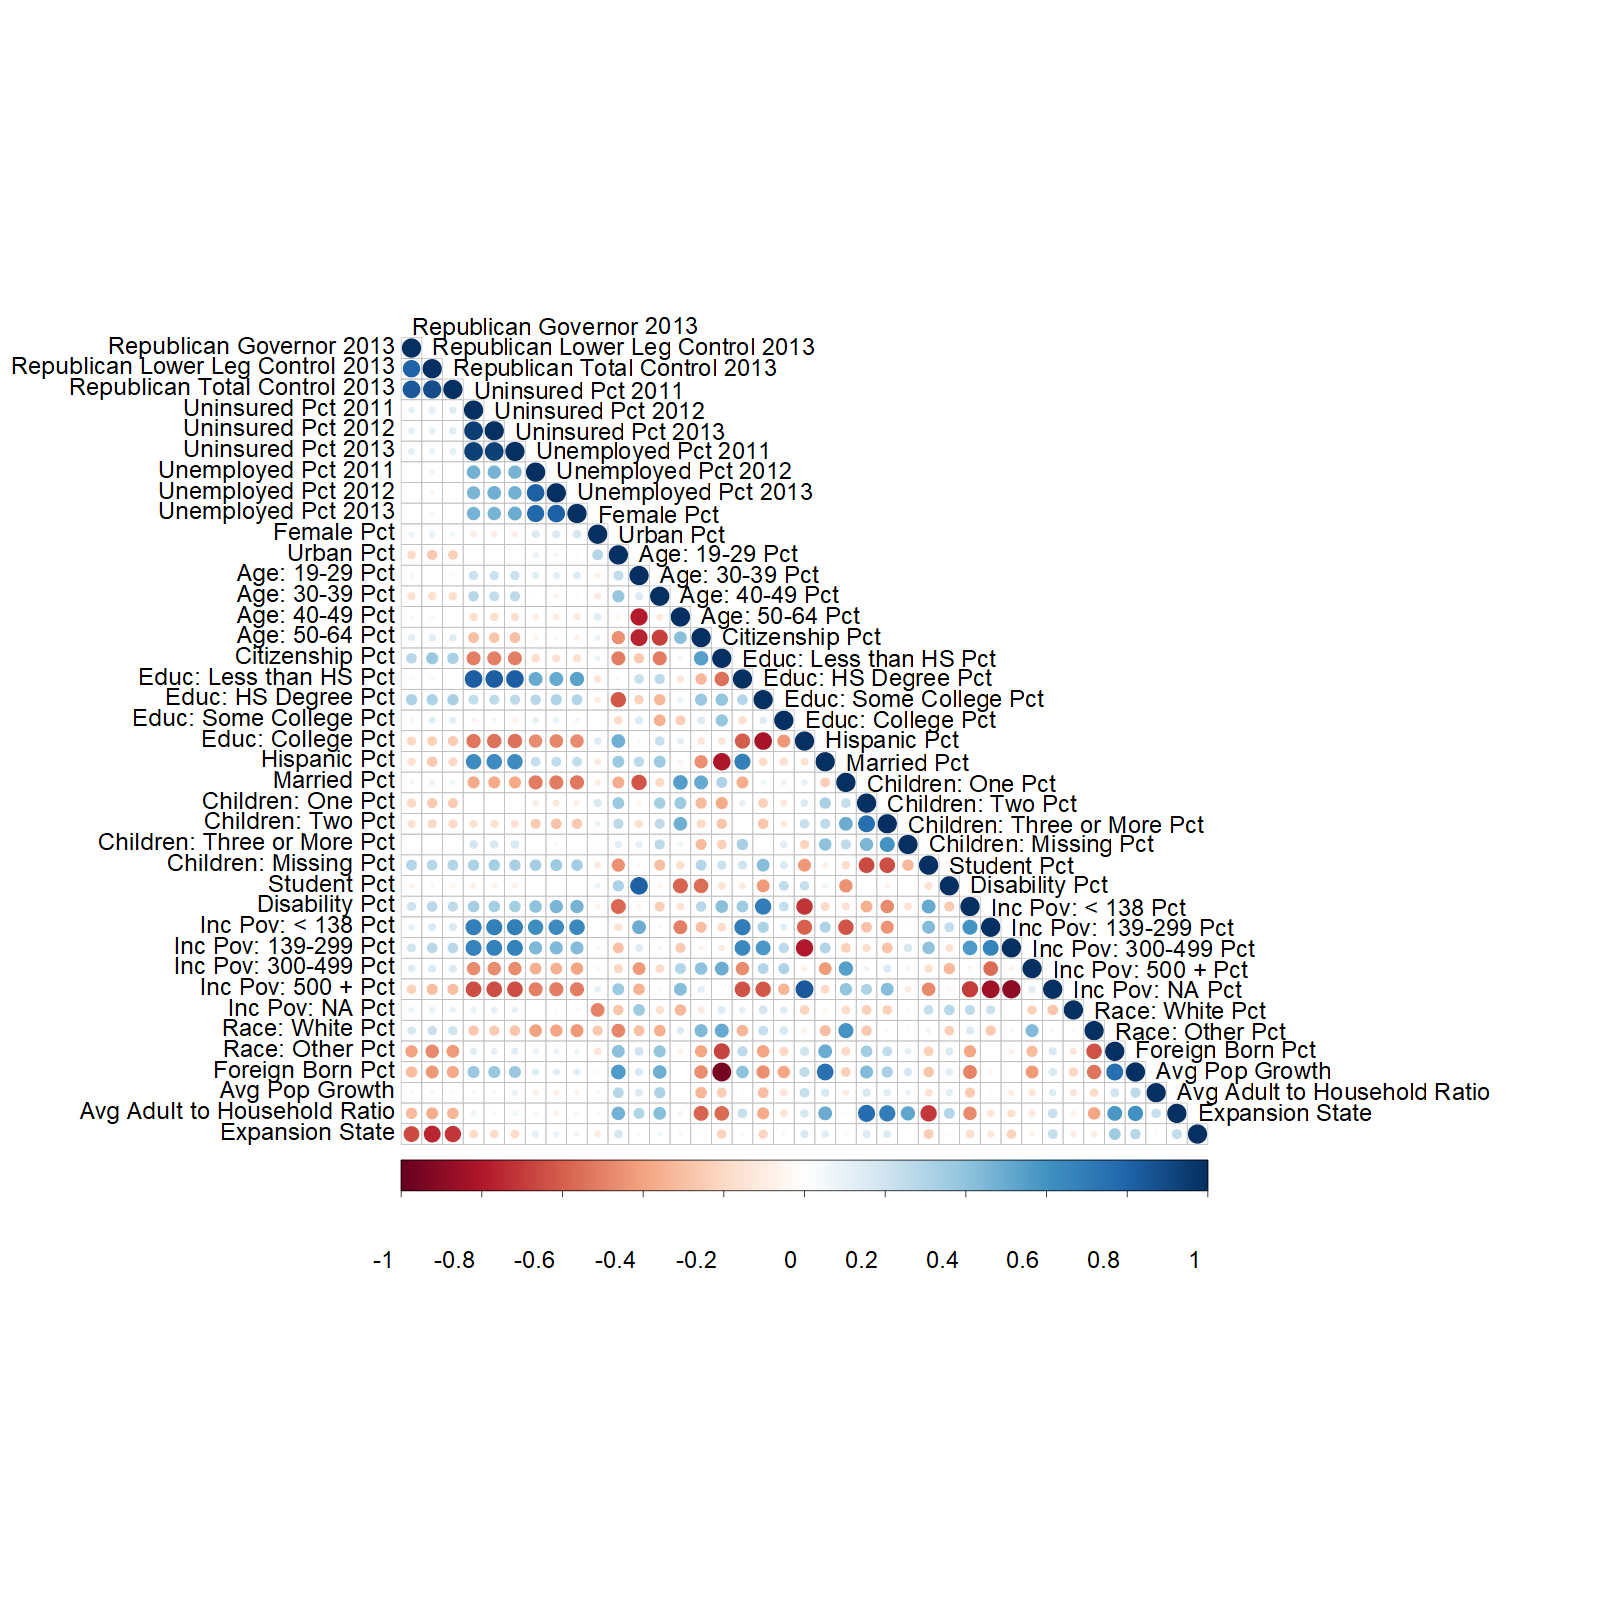
\includegraphics[scale=0.25]{01_Plots/correlation-plot-c1-sigma-zero.png}
\end{center}
\end{figure}

\clearpage

\clearpage

\begin{landscape}

\section{Weight Diagnostics}
\label{ssec:balancetables}

Table~\ref{tab:baltab1} displays the differences between the weighted mean covariate values of the expansion region and the mean of the non-expansion region for our primary dataset and with the early expansion states excluded (calculated using our the homogeneous covariate adjustments). The weights presented here are for the H-SBW estimator. The values under each column are in the following format: (unweighted difference, weighted difference). ``Primary'' and ``Early excluded'' refer to the primary dataset and those that exclude the early expansion states. ``Percent'' indicates that the differences displayed are in percentage points while ``Standardized'' indicates that the standardized mean differences are displayed. Additional results are available on request.

\begin{table}[h!]
\centering
    \caption{Balance table: percent and standardized mean differences, H-SBW weights}
    \label{tab:baltab1}
\begin{tabular}{lllll}
  \hline
Variables & Preferred (Percent) & Preferred (Standardized) & Early excluded (Percent) & Early excluded (Standardized) \\ 
  \hline
Age: 19-29 Pct & (-0.34, -0.34) & (-0.05, -0.05) & (-0.62, -0.21) & (-0.09, -0.03) \\ 
  Age: 30-39 Pct & (0.36, 0.17) & (0.1, 0.05) & (-0.04, 0.32) & (-0.01, 0.09) \\ 
  Age: 40-49 Pct & (0.19, -0.3) & (0.06, -0.1) & (-0.01, -0.44) & (0, -0.15) \\ 
  Avg Adult to Household Ratio & (11.29, -0.04) & (0.37, 0) & (3.37, 0.1) & (0.13, 0) \\ 
  Citizenship Pct & (-3.61, -1.59) & (-0.33, -0.15) & (-0.24, -1.45) & (-0.03, -0.16) \\ 
  Disability Pct & (-1.45, 0.52) & (-0.27, 0.1) & (-0.17, 0.63) & (-0.03, 0.11) \\ 
  Educ: HS Degree Pct & (-3.37, 0.54) & (-0.32, 0.05) & (-1.02, 0.64) & (-0.1, 0.06) \\ 
  Educ: Less than HS Pct & (-0.37, 0.83) & (-0.04, 0.1) & (-1.22, 0.76) & (-0.16, 0.1) \\ 
  Educ: Some College Pct & (-0.35, 0.4) & (-0.05, 0.06) & (0.36, 0.57) & (0.05, 0.08) \\ 
  Female Pct & (-0.34, -0.64) & (-0.16, -0.3) & (-0.25, -1) & (-0.12, -0.48) \\ 
  Foreign Born Pct & (7.6, 2) & (0.42, 0.11) & (1.02, 2) & (0.07, 0.13) \\ 
  Uninsured Pct 2011 & (-3.08, 0.05) & (-0.28, 0) & (-3.51, -0.05) & (-0.34, 0) \\ 
  Uninsured Pct 2012 & (-3, -0.05) & (-0.27, 0) & (-3.4, 0.05) & (-0.33, 0) \\ 
  Uninsured Pct 2013 & (-2.99, -0.05) & (-0.27, 0) & (-3.45, -0.05) & (-0.34, 0) \\ 
  Hispanic Pct & (4.46, 1) & (0.2, 0.04) & (-1.35, 1) & (-0.07, 0.05) \\ 
  Inc Pov: $<$ 138 Pct & (-2.05, 0.63) & (-0.19, 0.06) & (-1.33, 0.12) & (-0.12, 0.01) \\ 
  Inc Pov: 139-299 Pct & (-2.45, 0.65) & (-0.35, 0.09) & (-1.53, 0.5) & (-0.23, 0.08) \\ 
  Inc Pov: 300-499 Pct & (-0.59, -0.18) & (-0.12, -0.04) & (0.28, -0.18) & (0.06, -0.04) \\ 
  Inc Pov: 500 + Pct & (5.58, -1.3) & (0.35, -0.08) & (2.9, -1.23) & (0.2, -0.08) \\ 
  Married Pct & (-0.76, -0.43) & (-0.07, -0.04) & (-0.21, -0.53) & (-0.02, -0.05) \\ 
  Children: Missing Pct & (-3.25, -1) & (-0.36, -0.11) & (-1.99, -0.1) & (-0.21, -0.01) \\ 
  Children: One Pct & (0.7, -0.14) & (0.25, -0.05) & (0.11, -0.31) & (0.04, -0.12) \\ 
  Avg Pop Growth & (-0.09, -0.21) & (-0.07, -0.18) & (-0.26, -0.19) & (-0.22, -0.16) \\ 
  Race: White Pct & (-4.02, 1) & (-0.16, 0.04) & (0.09, 1) & (0, 0.04) \\ 
  Republican Governor 2013 & (-64.78, -25) & (-1.28, -0.5) & (-54.46, -24.87) & (-1.02, -0.47) \\ 
  Republican Lower Leg Control 2013 & (-74.72, -25) & (-1.69, -0.57) & (-56.67, -23.6) & (-1.12, -0.47) \\ 
  Republican Total Control 2013 & (-71.3, -25) & (-1.45, -0.51) & (-56.47, -25) & (-1.02, -0.45) \\ 
  Student Pct & (0.25, -0.5) & (0.04, -0.08) & (0.11, -0.25) & (0.02, -0.04) \\ 
  Children: Three or More Pct & (0, -0.21) & (0, -0.08) & (-0.17, -0.26) & (-0.07, -0.11) \\ 
  Children: Two Pct & (0.76, -0.31) & (0.23, -0.09) & (0.17, -0.37) & (0.05, -0.12) \\ 
  Unemployed Pct 2011 & (0.82, 0.15) & (0.18, 0.03) & (0.68, 0.15) & (0.15, 0.03) \\ 
  Unemployed Pct 2012 & (0.63, -0.03) & (0.14, -0.01) & (0.47, -0.03) & (0.11, -0.01) \\ 
  Unemployed Pct 2013 & (0.42, -0.15) & (0.11, -0.04) & (0.22, -0.15) & (0.06, -0.04) \\ 
  Urban Pct & (8.28, -2) & (0.26, -0.06) & (2.79, -2) & (0.08, -0.06) \\ 
   \hline
\end{tabular}
    \begin{tablenotes}
      \small
      \item The values displayed in each cell are the (weighted, unweighted) differences. The columns containing ``Standardized'' reflect the standardized mean differences while ``percent'' indicates the mean differences in percentage points. The columns containing ``Preferred'' indicate that this is for our primary analysis while ``Early excluded'' is for our analysis that excludes the early expansion states.
    \end{tablenotes}
\end{table}

Figure~\ref{fig:weightsbystatec2} display the weights summed by states when excluding the early expansion states for the H-SBW and BC-HSBW estimators.

\begin{figure}[H]
\begin{center}
    \caption{Total weights summed by state, early expansion removed}
    \label{fig:weightsbystatec2}
    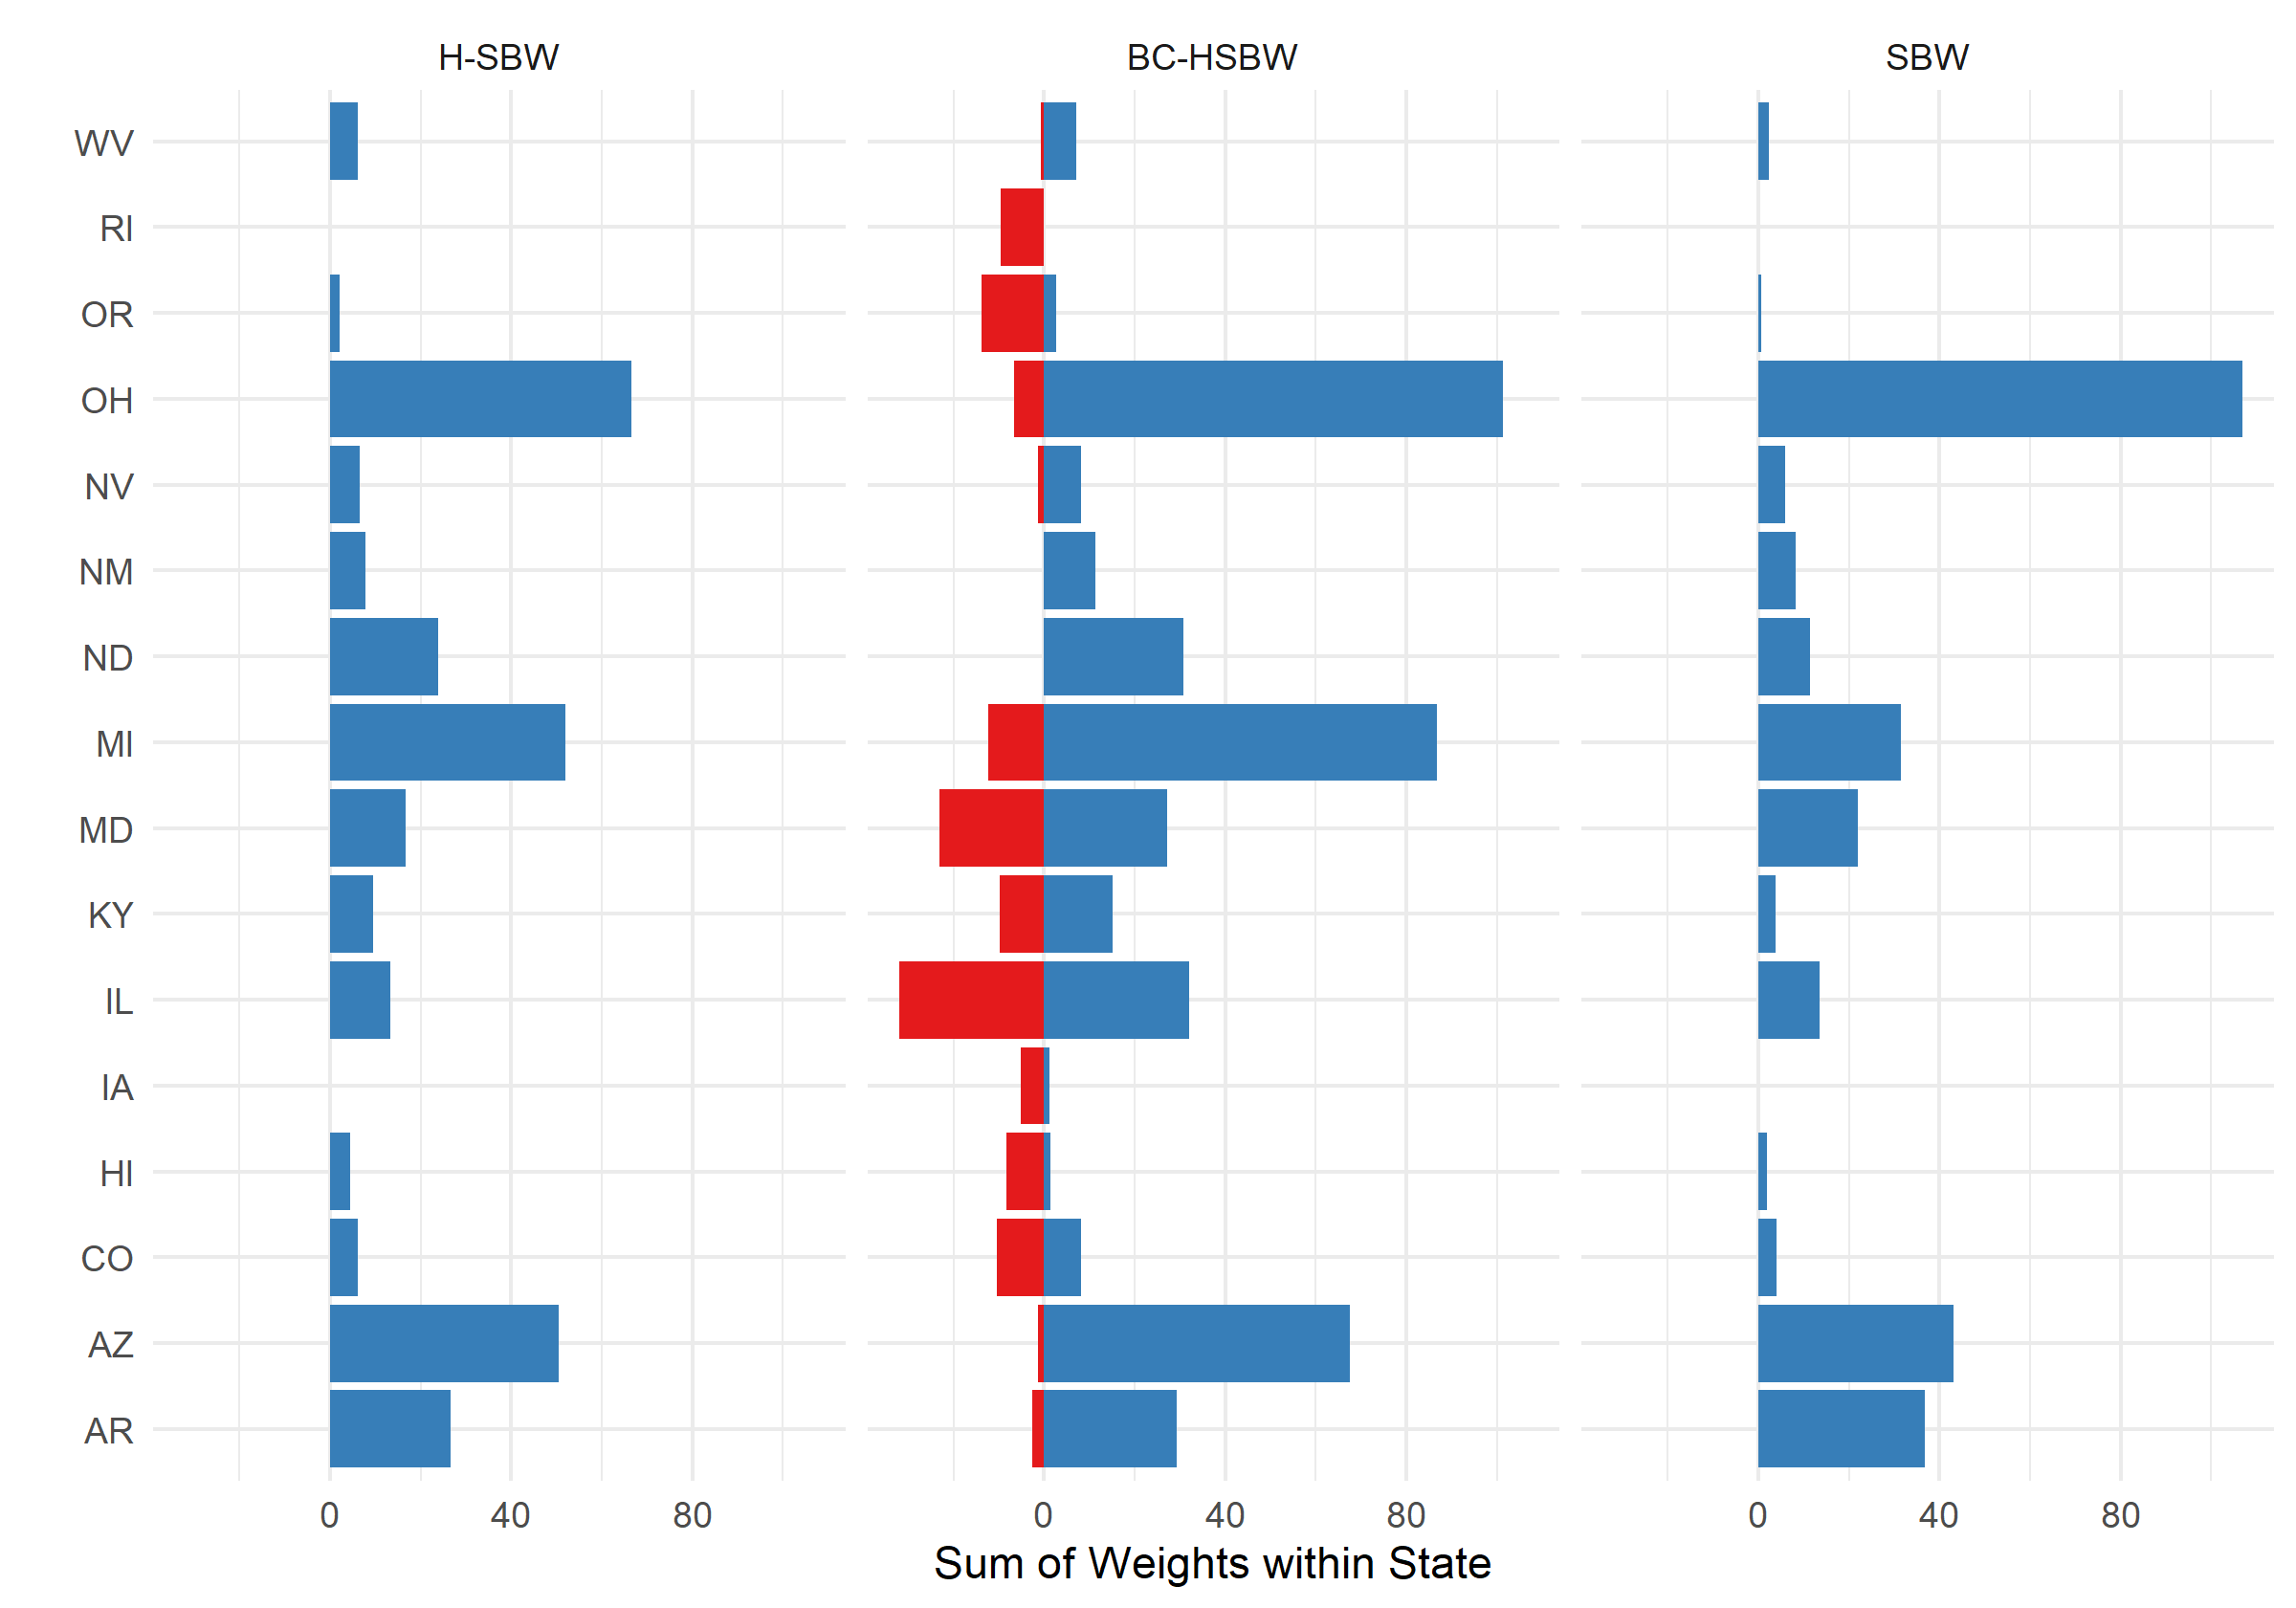
\includegraphics[scale=0.5]{01_Plots/weights-by-state-sbw-hsbw-c2-color.png}
\end{center}
\end{figure}
\end{landscape}
\clearpage

\clearpage

\section{Additional Results}
\label{ssec:allresults}

Table~\ref{tab:confintmain} displays the point estimates from all estimators as well as confidence intervals calculated either (a) leave-one-state-out jackknife on the adjusted dataset (CI (states)); (b) leave-one-state-out jackknife repeating the entire adjusted leaving each state out (CI (proc)). This table also includes all analyses calculated on a second version of the adjusted data where we use a common $\kappa$ for all values (sigma\_uu\_avg), which is the adjustment suggested by \cite{carroll2006measurement}. Notice that the confidence intervals are identical for ``sigma\_zero'' because this is the unadjusted dataset. ``sigma\_uu\_i'' is our preferred covariate adjustment.

\begin{table}[ht]
\centering
\caption{Point estimates and confidence intervals, primary dataset}
\label{tab:confintmain}
\begin{tabular}{llrll}
  \hline
Weight type & Sigma estimate & Psihat & CI (states) & CI (proc) \\ 
  \hline
H-SBW & sigma\_uu\_i & -2.17 & (-3.41, -0.94) & (-3.42, -0.92) \\ 
  H-SBW & sigma\_uu\_avg & -2.25 & (-3.51, -0.99) & (-3.35, -1.14) \\ 
  H-SBW & sigma\_zero & -2.35 & (-3.09, -1.61) & (-3.09, -1.61) \\ 
  BC-HSBW & sigma\_uu\_i & -2.13 & (-3.55, -0.71) & (-3.42, -0.84) \\ 
  BC-HSBW & sigma\_uu\_avg & -2.17 & (-3.57, -0.78) & (-3.39, -0.96) \\ 
  BC-HSBW & sigma\_zero & -2.40 & (-3.33, -1.46) & (-3.33, -1.46) \\ 
  SBW & sigma\_uu\_i & -2.24 & (-3.50, -0.99) & (-3.51, -0.97) \\ 
  SBW & sigma\_uu\_avg & -2.30 & (-3.67, -0.92) & (-3.45, -1.15) \\ 
  SBW & sigma\_zero & -2.40 & (-3.10, -1.69) & (-3.10, -1.69) \\ 
  BC-SBW & sigma\_uu\_i & -2.12 & (-3.15, -1.10) & (-3.11, -1.14) \\ 
  BC-SBW & sigma\_uu\_avg & -2.17 & (-3.25, -1.08) & (-3.22, -1.12) \\ 
  BC-SBW & sigma\_zero & -2.36 & (-2.93, -1.80) & (-2.93, -1.80) \\ 
   \hline
\end{tabular}
\end{table}

Table~\ref{tab:ptests} presents all point estimates from estimators that we calculated. The ``Var subset`` column indicates which variables were excluded from the estimation: 0 excludes no variables; 1 removes Republican governance indicators; 2 pre-treatment uninsurance and unemployment rates; 3 urban, age, education, citizenship, marital status, student, disability, or female; 4 race, ethnicity, income, foreign born; 5 children, population growth, and household to person ratio. We see that the largest changes generally occur when excluding the pre-treatment uninsurance and unemployment rates. This is not surprising: controlling for the other covariates, the pre-treatment uninsurance rate was substantially lower in the treated region compared to the control region. Given that pre-treatment uninsurance rates are highly correlated with post-treatment rates, we find that this comparison leads to a larger absolute magnitude point estimate, highlighting the need to control for these covariates.

%Wed Jan 13 15:24:43 2021
\begin{table}[ht]
\centering
\caption{Point estimates for all specifications}
\label{tab:ptests}
\begin{tabular}{rlrrrr}
  \hline
Variable subset & Sigma estimate & H-SBW & BC-HSBW & SBW & BC-SBW \\ 
  \hline
0 & sigma\_uu\_i & -2.17 & -2.13 & -2.24 & -2.12 \\ 
  0 & sigma\_uu\_avg & -2.25 & -2.17 & -2.30 & -2.17 \\ 
  0 & sigma\_zero & -2.35 & -2.40 & -2.40 & -2.36 \\ 
  1 & sigma\_uu\_i & -2.85 & -2.87 & -3.00 & -2.76 \\ 
  1 & sigma\_uu\_avg & -2.86 & -2.86 & -2.99 & -2.75 \\ 
  1 & sigma\_zero & -3.00 & -3.09 & -3.07 & -2.92 \\ 
  2 & sigma\_uu\_i & -5.73 & -5.05 & -5.24 & -4.70 \\ 
  2 & sigma\_uu\_avg & -5.73 & -5.05 & -5.24 & -4.70 \\ 
  2 & sigma\_zero & -5.73 & -5.13 & -5.24 & -4.77 \\ 
  3 & sigma\_uu\_i & -2.17 & -2.00 & -2.24 & -2.00 \\ 
  3 & sigma\_uu\_avg & -2.25 & -2.06 & -2.29 & -2.06 \\ 
  3 & sigma\_zero & -2.34 & -2.17 & -2.40 & -2.15 \\ 
  4 & sigma\_uu\_i & -2.35 & -2.39 & -2.29 & -2.30 \\ 
  4 & sigma\_uu\_avg & -2.39 & -2.39 & -2.32 & -2.32 \\ 
  4 & sigma\_zero & -2.45 & -2.59 & -2.43 & -2.49 \\ 
  5 & sigma\_uu\_i & -2.17 & -2.19 & -2.26 & -2.21 \\ 
  5 & sigma\_uu\_avg & -2.25 & -2.24 & -2.33 & -2.27 \\ 
  5 & sigma\_zero & -2.35 & -2.44 & -2.42 & -2.47 \\ 
   \hline
\end{tabular}
\end{table}

Table ~\ref{tab:confintmainc2} and Table~\ref{tab:secondaryptests} are identical to the structure of the previous two tables except we exclude the ``early expansion states'' from the pool of expansion state matches. 

\begin{table}[ht]
\centering
\caption{Point estimates and confidence intervals, early expansion excluded}
\label{tab:confintmainc2}
\begin{tabular}{llrll}
  \hline
Weight type & Sigma estimate & Psihat & CI (states) & CI (proc) \\ 
  \hline
H-SBW & sigma\_uu\_i & -2.05 & (-3.10, -1.00) & (-3.05, -1.05) \\ 
  H-SBW & sigma\_uu\_avg & -2.13 & (-3.20, -1.05) & (-3.17, -1.08) \\ 
  H-SBW & sigma\_zero & -2.29 & (-2.90, -1.69) & (-2.90, -1.69) \\ 
  BC-HSBW & sigma\_uu\_i & -2.14 & (-3.63, -0.64) & (-3.48, -0.80) \\ 
  BC-HSBW & sigma\_uu\_avg & -2.19 & (-3.65, -0.73) & (-3.57, -0.81) \\ 
  BC-HSBW & sigma\_zero & -2.50 & (-3.66, -1.33) & (-3.66, -1.33) \\ 
  SBW & sigma\_uu\_i & -1.91 & (-2.91, -0.91) & (-2.79, -1.03) \\ 
  SBW & sigma\_uu\_avg & -2.01 & (-3.02, -1.00) & (-2.83, -1.19) \\ 
  SBW & sigma\_zero & -2.20 & (-2.69, -1.71) & (-2.69, -1.71) \\ 
  BC-SBW & sigma\_uu\_i & -1.97 & (-3.49, -0.44) & (-3.27, -0.66) \\ 
  BC-SBW & sigma\_uu\_avg & -2.04 & (-3.59, -0.50) & (-3.39, -0.70) \\ 
  BC-SBW & sigma\_zero & -2.34 & (-3.44, -1.25) & (-3.44, -1.25) \\ 
   \hline
\end{tabular}
\end{table}

\begin{table}[ht]
\centering
   \caption{Point estimates for all specifications, early expansion excluded}
    \label{tab:secondaryptests}
\begin{tabular}{rlrrrr}
  \hline
Variable subset & Sigma estimate & H-SBW & BC-HSBW & SBW & BC-SBW \\ 
  \hline
0 & sigma\_uu\_i & -2.05 & -2.14 & -1.91 & -1.97 \\ 
  0 & sigma\_uu\_avg & -2.13 & -2.19 & -2.01 & -2.04 \\ 
  0 & sigma\_zero & -2.29 & -2.50 & -2.20 & -2.34 \\ 
  1 & sigma\_uu\_i & -2.85 & -2.99 & -2.85 & -2.86 \\ 
  1 & sigma\_uu\_avg & -2.86 & -2.98 & -2.86 & -2.86 \\ 
  1 & sigma\_zero & -3.05 & -3.18 & -2.96 & -2.99 \\ 
  2 & sigma\_uu\_i & -5.55 & -4.46 & -5.02 & -4.52 \\ 
  2 & sigma\_uu\_avg & -5.55 & -4.73 & -5.01 & -4.53 \\ 
  2 & sigma\_zero & -5.55 & -4.78 & -5.01 & -4.56 \\ 
  3 & sigma\_uu\_i & -2.05 & -2.03 & -1.91 & -1.89 \\ 
  3 & sigma\_uu\_avg & -2.13 & -2.10 & -2.00 & -1.97 \\ 
  3 & sigma\_zero & -2.27 & -2.22 & -2.20 & -2.13 \\ 
  4 & sigma\_uu\_i & -2.27 & -2.24 & -2.15 & -2.00 \\ 
  4 & sigma\_uu\_avg & -2.35 & -2.28 & -2.23 & -2.04 \\ 
  4 & sigma\_zero & -2.36 & -2.62 & -2.28 & -2.45 \\ 
  5 & sigma\_uu\_i & -2.05 & -2.20 & -1.91 & -2.03 \\ 
  5 & sigma\_uu\_avg & -2.13 & -2.26 & -1.99 & -2.11 \\ 
  5 & sigma\_zero & -2.29 & -2.45 & -2.19 & -2.36 \\ 
   \hline
\end{tabular}
\end{table}

Table~\ref{tab:loostatec1} and Table~\ref{tab:loostatec2} present point estimates for the leave-one-state out analysis for our preferred estimator, H-SBW calculated on our preferred covariate adjustment for the primary dataset and when excluding early expansion states.

\begin{table}[ht]
\centering
   \caption{Leave-one-state-out point estimates, primary dataset, preferred adjustment}
    \label{tab:loostatec1}
\begin{tabular}{lrlrl}
  \hline
State & Psihat (0) & None (states, proc) & Psihat (1) & Repub (states, proc) \\ 
  \hline
AR & -2.17 & (-2.34, -2.38) & -2.85 & (-2.81, -2.80) \\ 
  AZ & -2.17 & (-2.21, -2.24) & -2.85 & (-2.86, -2.86) \\ 
  CA & -2.17 & (-1.99, -2.02) & -2.85 & (-2.77, -2.76) \\ 
  CO & -2.17 & (-2.17, -2.23) & -2.85 & (-2.84, -2.84) \\ 
  CT & -2.17 & (-2.17, -2.15) & -2.85 & (-2.83, -2.82) \\ 
  HI & -2.17 & (-2.15, -2.14) & -2.85 & (-2.77, -2.78) \\ 
  IA & -2.17 & (-2.09, -2.07) & -2.85 & (-2.83, -2.84) \\ 
  IL & -2.17 & (-2.16, -2.24) & -2.85 & (-2.83, -2.84) \\ 
  KY & -2.17 & (-2.02, -1.95) & -2.85 & (-2.57, -2.52) \\ 
  MD & -2.17 & (-2.25, -2.27) & -2.85 & (-2.94, -2.94) \\ 
  MI & -2.17 & (-2.10, -2.18) & -2.85 & (-2.89, -2.92) \\ 
  MN & -2.17 & (-2.17, -2.19) & -2.85 & (-2.84, -2.86) \\ 
  ND & -2.17 & (-2.23, -2.26) & -2.85 & (-2.84, -2.84) \\ 
  NH & -2.17 & (-2.18, -2.21) & -2.85 & (-2.98, -2.99) \\ 
  NJ & -2.17 & (-2.26, -2.25) & -2.85 & (-2.99, -3.03) \\ 
  NM & -2.17 & (-2.16, -2.22) & -2.85 & (-2.76, -2.77) \\ 
  NV & -2.17 & (-2.21, -2.24) & -2.85 & (-2.89, -2.88) \\ 
  OH & -2.17 & (-2.70, -2.68) & -2.85 & (-3.00, -2.98) \\ 
  OR & -2.17 & (-2.17, -2.25) & -2.85 & (-2.80, -2.84) \\ 
  RI & -2.17 & (-2.17, -2.15) & -2.85 & (-2.81, -2.81) \\ 
  WA & -2.17 & (-2.10, -2.11) & -2.85 & (-2.78, -2.77) \\ 
  WV & -2.17 & (-2.16, -2.18) & -2.85 & (-2.8, -2.78) \\ 
   \hline
\end{tabular}
\end{table}

\begin{table}[ht]
\centering
   \caption{Leave-one-state-out point estimates, early expansion excluded, preferred adjustment}
    \label{tab:loostatec2}
\begin{tabular}{lrlrl}
  \hline
State & Psihat (0) & None (states, proc) & Psihat (1) & Repub (states, proc) \\ 
  \hline
AR & -2.05 & (-2.15, -2.16) & -2.85 & (-2.77, -2.76) \\ 
  AZ & -2.05 & (-1.82, -1.88) & -2.85 & (-2.87, -2.86) \\ 
  CO & -2.05 & (-2.07, -2.09) & -2.85 & (-2.84, -2.83) \\ 
  HI & -2.05 & (-2.01, -1.99) & -2.85 & (-2.71, -2.73) \\ 
  IA & -2.05 & (-1.98, -1.95) & -2.85 & (-2.85, -2.86) \\ 
  IL & -2.05 & (-2.03, -2.01) & -2.85 & (-2.8, -2.79) \\ 
  KY & -2.05 & (-1.87, -1.8) & -2.85 & (-2.59, -2.54) \\ 
  MD & -2.05 & (-2.18, -2.15) & -2.85 & (-2.97, -2.96) \\ 
  MI & -2.05 & (-1.96, -2) & -2.85 & (-2.92, -2.96) \\ 
  ND & -2.05 & (-2.02, -2.04) & -2.85 & (-2.84, -2.84) \\ 
  NH & -2.05 & (-2.05, -2.06) & -2.85 & (-3.02, -3.03) \\ 
  NM & -2.05 & (-1.99, -1.97) & -2.85 & (-2.72, -2.75) \\ 
  NV & -2.05 & (-2.15, -2.15) & -2.85 & (-2.93, -2.92) \\ 
  OH & -2.05 & (-2.43, -2.38) & -2.85 & (-3.03, -3.02) \\ 
  OR & -2.05 & (-2.05, -2.11) & -2.85 & (-2.81, -2.84) \\ 
  RI & -2.05 & (-2.05, -2.05) & -2.85 & (-2.80, -2.80) \\ 
  WV & -2.05 & (-2.06, -2.06) & -2.85 & (-2.83, -2.81) \\ 
   \hline
\end{tabular}
\end{table}

Table~\ref{tab:oateconfint} displays point estimates and confidence intervals for the primary point estimates for the OATE. We display the confidence intervals calculated using both the leave-one-out-states conditional on the covariate adjustment (CI (states)) and recalculating the covariate adjustment for the OATE (CI (proc)). 

\begin{table}[ht]
\centering
\caption{OATE primary results inference}
\label{tab:oateconfint}
\begin{tabular}{rllll}
  \hline
Psihat & Sigma estimate & Dataset & CI (states) & CI (proc) \\ 
  \hline
-1.74 & sigma\_uu\_i\_modeled & c1 & (-2.35, -1.14) & (-2.48, -1.00) \\ 
  -1.67 & sigma\_uu\_avg & c1 & (-2.34, -0.99) & (-2.52, -0.81) \\ 
  -1.80 & sigma\_zero & c1 & (-2.50, -1.10) & (-2.50, -1.10) \\ 
  -1.89 & sigma\_uu\_i\_modeled & c2 & (-2.47, -1.32) & (-2.54, -1.24) \\ 
  -1.80 & sigma\_uu\_avg & c2 & (-2.43, -1.17) & (-2.57, -1.03) \\ 
  -1.95 & sigma\_zero & c2 & (-2.65, -1.25) & (-2.65, -1.25) \\ 
   \hline
\end{tabular}
\end{table}

Table~\ref{tab:oatesensitive} presents all point estimates calculate using the overlap weights. Dataset ``c1'' refers to the primary dataset and dataset ``c2'' removes the early expansion states. The numeric column names refer to the covariate group excluded (covariate groups described above).

\begin{table}[ht]
\centering
\caption{OATE all point estimates}
\label{tab:oatesensitive}
\begin{tabular}{llrrrrrr}
  \hline
Sigma estimate & Dataset & 0 & 1 & 2 & 3 & 4 & 5 \\ 
  \hline
sigma\_uu\_i & c1 & -1.64 & -2.60 & -2.96 & -1.86 & -1.86 & -1.77 \\ 
  sigma\_uu\_i & c2 & -1.81 & -2.53 & -3.10 & -2.18 & -2.04 & -1.96 \\ 
  sigma\_avg & c1 & -1.58 & -2.62 & -2.85 & -1.76 & -1.76 & -1.78 \\ 
  sigma\_avg & c2 & -1.74 & -2.54 & -3.00 & -2.10 & -1.96 & -1.95 \\ 
  sigma\_zero & c1 & -1.80 & -2.55 & -3.11 & -1.98 & -1.94 & -1.83 \\ 
  sigma\_zero & c2 & -1.95 & -2.51 & -3.25 & -2.12 & -2.10 & -2.00 \\ 
   \hline
\end{tabular}
\end{table}

Table~\ref{tab:rdiffc1} and ~\ref{tab:rdiffc2} display the quantiles of the distribution $\hat{\Delta}_v^1$ estimates when leaving out each state for the primary dataset and removing the early expansion states. The ``resample'' column indicates whether the entire adjustment procedure was recalculated (``proc'') or whether we left out each state conditional on the adjustment (``states''). Table~\ref{tab:hte} displays the estimated linear combination of model coefficients on the Republican governance indicators with 95 percent confidence intervals (standard errors clustered at the state level). The ``Weights'' column represents whether the regressions were weighted; we ran two versions, an unweighted regression and one using the overlap weights.

\begin{table}[ht]
\centering
\label{tab:rdiffc1}
\caption{$\hat{\Delta}^1_v$ leave-one-state-out estimates, primary dataset}
\begin{tabular}{lllrrrrrr}
  \hline
Resample & Sigma estimate & Weight type & Original & 0\% & 25\% & 50\% & 75\% & 100\% \\ 
  \hline
states & sigma\_uu\_i\_modeled & H-SBW & -0.67 & -0.80 & -0.68 & -0.67 & -0.62 & -0.30 \\ 
  proc & sigma\_uu\_i\_modeled & H-SBW & -0.67 & -0.78 & -0.68 & -0.64 & -0.59 & -0.30 \\ 
  states & sigma\_uu\_i\_modeled & BC-HSBW & -0.74 & -0.87 & -0.77 & -0.71 & -0.69 & -0.26 \\ 
  proc & sigma\_uu\_i\_modeled & BC-HSBW & -0.74 & -0.85 & -0.76 & -0.70 & -0.67 & -0.34 \\ 
  states & sigma\_uu\_i\_modeled & SBW & -0.75 & -0.98 & -0.77 & -0.75 & -0.72 & -0.48 \\ 
  proc & sigma\_uu\_i\_modeled & SBW & -0.75 & -0.98 & -0.78 & -0.73 & -0.67 & -0.49 \\ 
  states & sigma\_uu\_i\_modeled & BC-SBW & -0.63 & -0.85 & -0.69 & -0.62 & -0.61 & -0.39 \\ 
  proc & sigma\_uu\_i\_modeled & BC-SBW & -0.63 & -0.82 & -0.68 & -0.64 & -0.59 & -0.35 \\ 
  states & sigma\_uu\_avg & H-SBW & -0.61 & -0.74 & -0.64 & -0.60 & -0.57 & -0.23 \\ 
  proc & sigma\_uu\_avg & H-SBW & -0.61 & -0.76 & -0.63 & -0.59 & -0.55 & -0.33 \\ 
  states & sigma\_uu\_avg & BC-HSBW & -0.69 & -0.83 & -0.73 & -0.68 & -0.64 & -0.24 \\ 
  proc & sigma\_uu\_avg & BC-HSBW & -0.69 & -0.83 & -0.73 & -0.66 & -0.63 & -0.39 \\ 
  states & sigma\_uu\_avg & SBW & -0.70 & -0.89 & -0.72 & -0.69 & -0.67 & -0.31 \\ 
  proc & sigma\_uu\_avg & SBW & -0.70 & -0.93 & -0.73 & -0.68 & -0.65 & -0.49 \\ 
  states & sigma\_uu\_avg & BC-SBW & -0.58 & -0.78 & -0.63 & -0.57 & -0.56 & -0.32 \\ 
  proc & sigma\_uu\_avg & BC-SBW & -0.58 & -0.81 & -0.63 & -0.58 & -0.55 & -0.28 \\ 
  states & sigma\_zero & H-SBW & -0.65 & -0.78 & -0.66 & -0.63 & -0.61 & -0.50 \\ 
  proc & sigma\_zero & H-SBW & -0.65 & -0.78 & -0.66 & -0.63 & -0.61 & -0.50 \\ 
  states & sigma\_zero & BC-HSBW & -0.70 & -0.88 & -0.74 & -0.68 & -0.64 & -0.50 \\ 
  proc & sigma\_zero & BC-HSBW & -0.70 & -0.88 & -0.74 & -0.68 & -0.64 & -0.50 \\ 
  states & sigma\_zero & SBW & -0.68 & -0.84 & -0.71 & -0.68 & -0.66 & -0.49 \\ 
  proc & sigma\_zero & SBW & -0.68 & -0.84 & -0.71 & -0.68 & -0.66 & -0.49 \\ 
  states & sigma\_zero & BC-SBW & -0.56 & -0.67 & -0.61 & -0.55 & -0.52 & -0.39 \\ 
  proc & sigma\_zero & BC-SBW & -0.56 & -0.67 & -0.61 & -0.55 & -0.52 & -0.39 \\ 
   \hline
\end{tabular}
\end{table}

\begin{table}[ht]
\label{tab:rdiffc2}
\caption{$\hat{\Delta}^1_v$ leave-one-state-out estimates, early expansion excluded}
\centering
\begin{tabular}{lllrrrrrr}
  \hline
Resample & Sigma estimate & Weight type & Original & 0\% & 25\% & 50\% & 75\% & 100\% \\ 
  \hline
states & sigma\_uu\_i\_modeled & H-SBW & -0.80 & -1.05 & -0.82 & -0.77 & -0.73 & -0.60 \\ 
  proc & sigma\_uu\_i\_modeled & H-SBW & -0.80 & -0.98 & -0.81 & -0.76 & -0.74 & -0.60 \\ 
  states & sigma\_uu\_i\_modeled & BC-HSBW & -0.85 & -1.13 & -0.96 & -0.83 & -0.76 & -0.45 \\ 
  proc & sigma\_uu\_i\_modeled & BC-HSBW & -0.85 & -1.05 & -0.94 & -0.83 & -0.77 & -0.53 \\ 
  states & sigma\_uu\_i\_modeled & SBW & -0.94 & -1.15 & -0.94 & -0.92 & -0.89 & -0.70 \\ 
  proc & sigma\_uu\_i\_modeled & SBW & -0.94 & -1.05 & -0.98 & -0.91 & -0.86 & -0.73 \\ 
  states & sigma\_uu\_i\_modeled & BC-SBW & -0.89 & -1.27 & -0.93 & -0.86 & -0.81 & -0.26 \\ 
  proc & sigma\_uu\_i\_modeled & BC-SBW & -0.89 & -1.19 & -0.96 & -0.86 & -0.81 & -0.37 \\ 
  states & sigma\_uu\_avg & H-SBW & -0.73 & -0.99 & -0.74 & -0.70 & -0.68 & -0.51 \\ 
  proc & sigma\_uu\_avg & H-SBW & -0.73 & -0.94 & -0.73 & -0.69 & -0.67 & -0.50 \\ 
  states & sigma\_uu\_avg & BC-HSBW & -0.79 & -1.10 & -0.87 & -0.78 & -0.69 & -0.42 \\ 
  proc & sigma\_uu\_avg & BC-HSBW & -0.79 & -1.01 & -0.89 & -0.73 & -0.69 & -0.46 \\ 
  states & sigma\_uu\_avg & SBW & -0.85 & -1.08 & -0.85 & -0.83 & -0.81 & -0.66 \\ 
  proc & sigma\_uu\_avg & SBW & -0.85 & -0.95 & -0.86 & -0.82 & -0.80 & -0.68 \\ 
  states & sigma\_uu\_avg & BC-SBW & -0.82 & -1.21 & -0.86 & -0.80 & -0.74 & -0.18 \\ 
  proc & sigma\_uu\_avg & BC-SBW & -0.82 & -1.09 & -0.86 & -0.76 & -0.74 & -0.26 \\ 
  states & sigma\_zero & H-SBW & -0.76 & -0.95 & -0.83 & -0.74 & -0.70 & -0.58 \\ 
  proc & sigma\_zero & H-SBW & -0.76 & -0.95 & -0.83 & -0.74 & -0.70 & -0.58 \\ 
  states & sigma\_zero & BC-HSBW & -0.69 & -1.00 & -0.83 & -0.70 & -0.60 & -0.39 \\ 
  proc & sigma\_zero & BC-HSBW & -0.69 & -1.00 & -0.83 & -0.70 & -0.60 & -0.39 \\ 
  states & sigma\_zero & SBW & -0.76 & -0.91 & -0.83 & -0.75 & -0.74 & -0.51 \\ 
  proc & sigma\_zero & SBW & -0.76 & -0.91 & -0.83 & -0.75 & -0.74 & -0.51 \\ 
  states & sigma\_zero & BC-SBW & -0.64 & -1.06 & -0.70 & -0.58 & -0.55 & -0.38 \\ 
  proc & sigma\_zero & BC-SBW & -0.64 & -1.06 & -0.70 & -0.58 & -0.55 & -0.38 \\ 
   \hline
\end{tabular}
\end{table}

\begin{table}[ht]
\caption{OLS HTE estimates}
\label{tab:hte}
\centering
\begin{tabular}{rllll}
  \hline
Estimate & Dataset & Sigma estimate & CI 95 & Weights \\ 
  \hline
  -1.76 & c1 & sigma\_uu\_i\_modeled & (-5.47, 1.94) & Overlap \\ 
  -1.67 & c1 & sigma\_uu\_avg & (-7.18, 3.84) & Overlap \\ 
  -1.97 & c1 & sigma\_zero & (-4.11, 0.17) & Overlap \\ 
  0.51 & c2 & sigma\_uu\_i\_modeled & (-6.00, 7.02) & Overlap \\ 
  -0.17 & c2 & sigma\_uu\_avg & (-8.17, 7.83) & Overlap \\ 
  -1.48 & c2 & sigma\_zero & (-3.51, 0.54) & Overlap \\ 
  0.10 & c1 & sigma\_uu\_i\_modeled & (-1.09, 1.30) & None \\ 
  0.61 & c1 & sigma\_uu\_avg & (-1.82, 3.04) & None \\ 
  -0.12 & c1 & sigma\_zero & (-0.90, 0.66) & None \\ 
  0.37 & c2 & sigma\_uu\_i\_modeled & (-0.9, 1.63) & None \\ 
  0.64 & c2 & sigma\_uu\_avg & (-1.77, 3.04) & None \\ 
  -0.11 & c2 & sigma\_zero & (-0.91, 0.68) & None \\ 
   \hline
\end{tabular}
\end{table}


%The synthetic controls approach chooses the $\gamma$ that minimizes the weighted L2-squared distance of the covariates using a diagonal weighting matrix $V$. $V$ is then chosen to minimize the mean-square error of the weighted difference in pre-treatment outcomes. Letting $Z_a$ be the matrix of pre-treatment outcomes for treatment group $A = a$, the synthetic controls algorithm solves the following optimization problem for a fixed $V$:

\begin{align}
\gamma(V) = \arg\min_{\tilde{\gamma}(V^\star)} = (\bar{X}_1 - X_0^T\tilde{\gamma})'V(\bar{X}_1 - X_0^T\tilde{\gamma}) 
\end{align}

This is the ``inner'' optimization. $V^\star$ is then determined in an ``outer'' optimization to minimize the imbalances in the pre-treatment outcomes $Z$:

\begin{align}
    V^\star = \arg\min_V (\bar{Z}_1 - Z_0^T\gamma(V))'(\bar{Z}_1 - Z_0^T\gamma(V))
\end{align}

In applications the covariate matrix $X_a$ may contain some elements of $Z_a$. In cases where $X_a$ contains all pre-treatment outcomes, \cite{kaul2015synthetic} has shown that the predictor weights $V^\star$ will give no weight to auxillary covariates (covariates that are not the pre-treatment outcomes), rendering these irrelevant to the model. 

While in practice $V$ is often learned on the same data as the weights, we consider the case where we use cross-validation to choose $V$, as proposed by \cite{abadie2015comparative}. Assume we can divide our pre-treatment data into a training data from periods $T = 1, ..., T - l - 1$, a validation period from periods $T - l, ..., T - 1$, and a post-treatment period at time $T$. To make this discussion more general, assume that we are evaluating a set of candidate models $\mathcal{M}$ on the validation data (where for the synthetic controls algorithm we can think of this as the set of all possible weighting matrices $V$). Let $\bar{Y}^a_{a', t}$ 
be the mean potential outcome under treatment $A = a$ for treatment group $A = a'$ at time $t$ (where $t$ occurs during the validation period). Let $\hat{\bar{Y}}^a_{a'', t}(m)$ be an estimator of that potential outcome at time $t$ using model $m$, which was trained during the training period using data from treatment group $A = a''$. Finally, let $\bar{Y}_{a'}^{a_T}$ be the post-treatment estimand, where $\hat{Y}^a_{a'', T}(m)$ is the estimator using model $m$ trained using validation period data. This learning procedure implicitly assumes that:

\begin{align*}
m^\star = \min_{m \in \mathcal{M}}\sum_{T - l}^{T-1}\|\hat{Y}^0_{0, t}(m) - \bar{Y}^0_{1, t}\| = \min_{m \in \mathcal{M}}\mathbb{E}\{\|\hat{Y}^0_{0, T}(m) - \bar{Y}^0_{1, T}\|\}
\end{align*}

In other words, we select our model using the empirical loss in the validation period as a proxy for the expected loss in the post-treatment time-period.\footnote{It is possible that multiple models in $\mathcal{M}$ either perfectly predict the pre-treatment outcomes, or predict them equally well. In this case we would require an additional criteria to choose the optimal model (see, e.g, \cite{becker2017cross}}. This makes intuitive sense in the typical synthetic controls setting where the estimand is the ETT since we observe $Y^0_{sct}$ for $t < T$. When synthetic controls are used to estimate the ETC, this strategy alone is insufficient as we never observe $Y^1_{sct}$ (or a mean-unbiased proxy) prior to treatment for any unit. We therefore cannot easily use pre-treatment outcomes to optimally select variables or determine relative covariate importance without stronger assumptions.

One such assumption is the following:

\begin{align*}\label{assumption:second}
m^\star = \min_{m \in \mathcal{M}}\sum_{T - l}^{T-1}\|\hat{Y}^0_{1, t}(m) - \hat{Y}^0_{0, t}\| = \min_{m \in \mathcal{M}}\mathbb{E}\{\|\hat{Y}^1_{1, T}(m) - \bar{Y}^1_{0, T}\|\}
\end{align*}

We call this assumption ``counterfactual risk invariance.'' In other words, we assume that the model that minimizes the validation-period risk also minimizes the post-treatment risk. We caution that this is a strong assumption for conducting any form of variable selection or covariate weighting in this setting. 

As a practical example, we highlight the potential confounding role of Republican governance for our counterfactual estimate. Republican governance is a strong predictor of a state's decision to expand Medicaid \cite{courtemanche2017early}. Moreover, existing evidence prior to Medicaid expansion showed that Medicaid take-up rates were lower in more conservative states \cite{sommers2012understanding}. However, when generating their synthetic control weights to estimate the ETT, \cite{courtemanche2017early} and \cite{kaestner2017effects} do not control for these factors. \footnote{\cite{courtemanche2017early} does control for Republican governor in their regression model and they find that it is a statistically significant predictor of 2013 uninsurance rates. One reason they may not control for this in the synthetic control model is practical: it is challenging to balance this covariate using control data without extrapolating from the data.} However, it is clear that if take-up rates depend on governance, we may expect this to be a strong confounder of $Y^1$ and hence confound the ETC, even if arguably it is not a confounder of $Y^0$ (and hence not a confounder for the ETT).

We demonstrate this in our application by conducting a variable importance analysis. Specifically, we remove the balance constraints from the Republican governance indicators and examine how our estimates of $\hat{\psi}^1$ change. Letting $\hat{\psi}^1_s$ be the estimate when removing the Republican governance indicators (or more generally, the covariate matrix $S$ where $X = (R, S)$). We subtract our original point estimate $\hat{\psi}^1_0$ from $\hat{\psi}^1_s$ to generate the difference $\hat{\Delta}^1$. This difference tells us about the direction of the bias our estimate of $\hat{\psi}^1$ would incur when we do attempt to constrain the imbalance in covariate $S$. Our hypothesis implies that we should expect $\hat{\Delta}_s^1 < 0$: that is, keeping all other covariates (roughly) fixed, we expect the predicted uninsurance rate will decrease when as the level of Republican governance decreases. In addition to the Republican governance indicators, we also examine four other covariate groups: pre-treatment uninsurance rates and pre-treatment unemployment rates, and three sets of different demographic indicators, which we detail in Appendix E.\footnote{We caution that our results do not imply that Republican governance is not an important confounder of $Y^0_{1, T}$ since we do not analyze this directly.} 

We point out that modeling the ETC requires greater justification of the covariates used to predict treatment response than for the ETT, and that using the standard synthetic controls variable weighting procedure is unlikely to be optimal for this purpose.\footnote{Our analysis assumes no unmeasured confounding and a linear model for $\mu_a$. By contrast, synthetic controls are frequently motivated by a linear factor model for $\mu_0$. \cite{abadie2010synthetic} and \cite{ferman2016revisiting} outline conditions where this method is consistent as the number of pre-treatment outcomes goes to infinity, in particular because the method balances the unobserved factor loadings. Analogous to our analysis, if we assume $\mu_{a, T}$ both follow a linear factor model, identification of the ETC requires that the unobserved factor loadings that confound $Y^1_T$ are the same that confound $Y^0_t$. Under this assumption, we might be able to show that the synthetic control estimator is consistent in this setting. However, the tuning procedure to determine the predictor weights may again be sub-optimal from a finite-sample bias perspective, depending again on how the covariates (or unobserved factors) that are most predictive of treatment response vary between treatment groups and on their associations with the potential outcomes.}

For our application, we constrain $\delta$ to be 0.05 percentage points (out of 100) for pre-treatment outcomes, 0.15 percentage points for pre-treatment unemployment rates, and 25 percentage points for the Republican governance indicators. We believe these covariates are most likely to predict treatment response. While we believe that Republican governance is an important covariate to balance, we are unable to reduce the constraints further given the support of the data. For the remaining covariates, we let $\delta$ be 0.5 percentage points for average population growth and household to adult ratio, 1 percentage point for female, Hispanic ethnicity, white race, age category, disability, and number of children category; 2 percentage points for urban, citizenship, education category, income-to-poverty category, student, and foreign-born, again choosing these constraints with respect to both feasibility and extreme weight concerns. 
\begin{figure}[H]
\begin{center}
    \caption{Estimator sensitivity to states}
    \label{fig:loostateplot}
    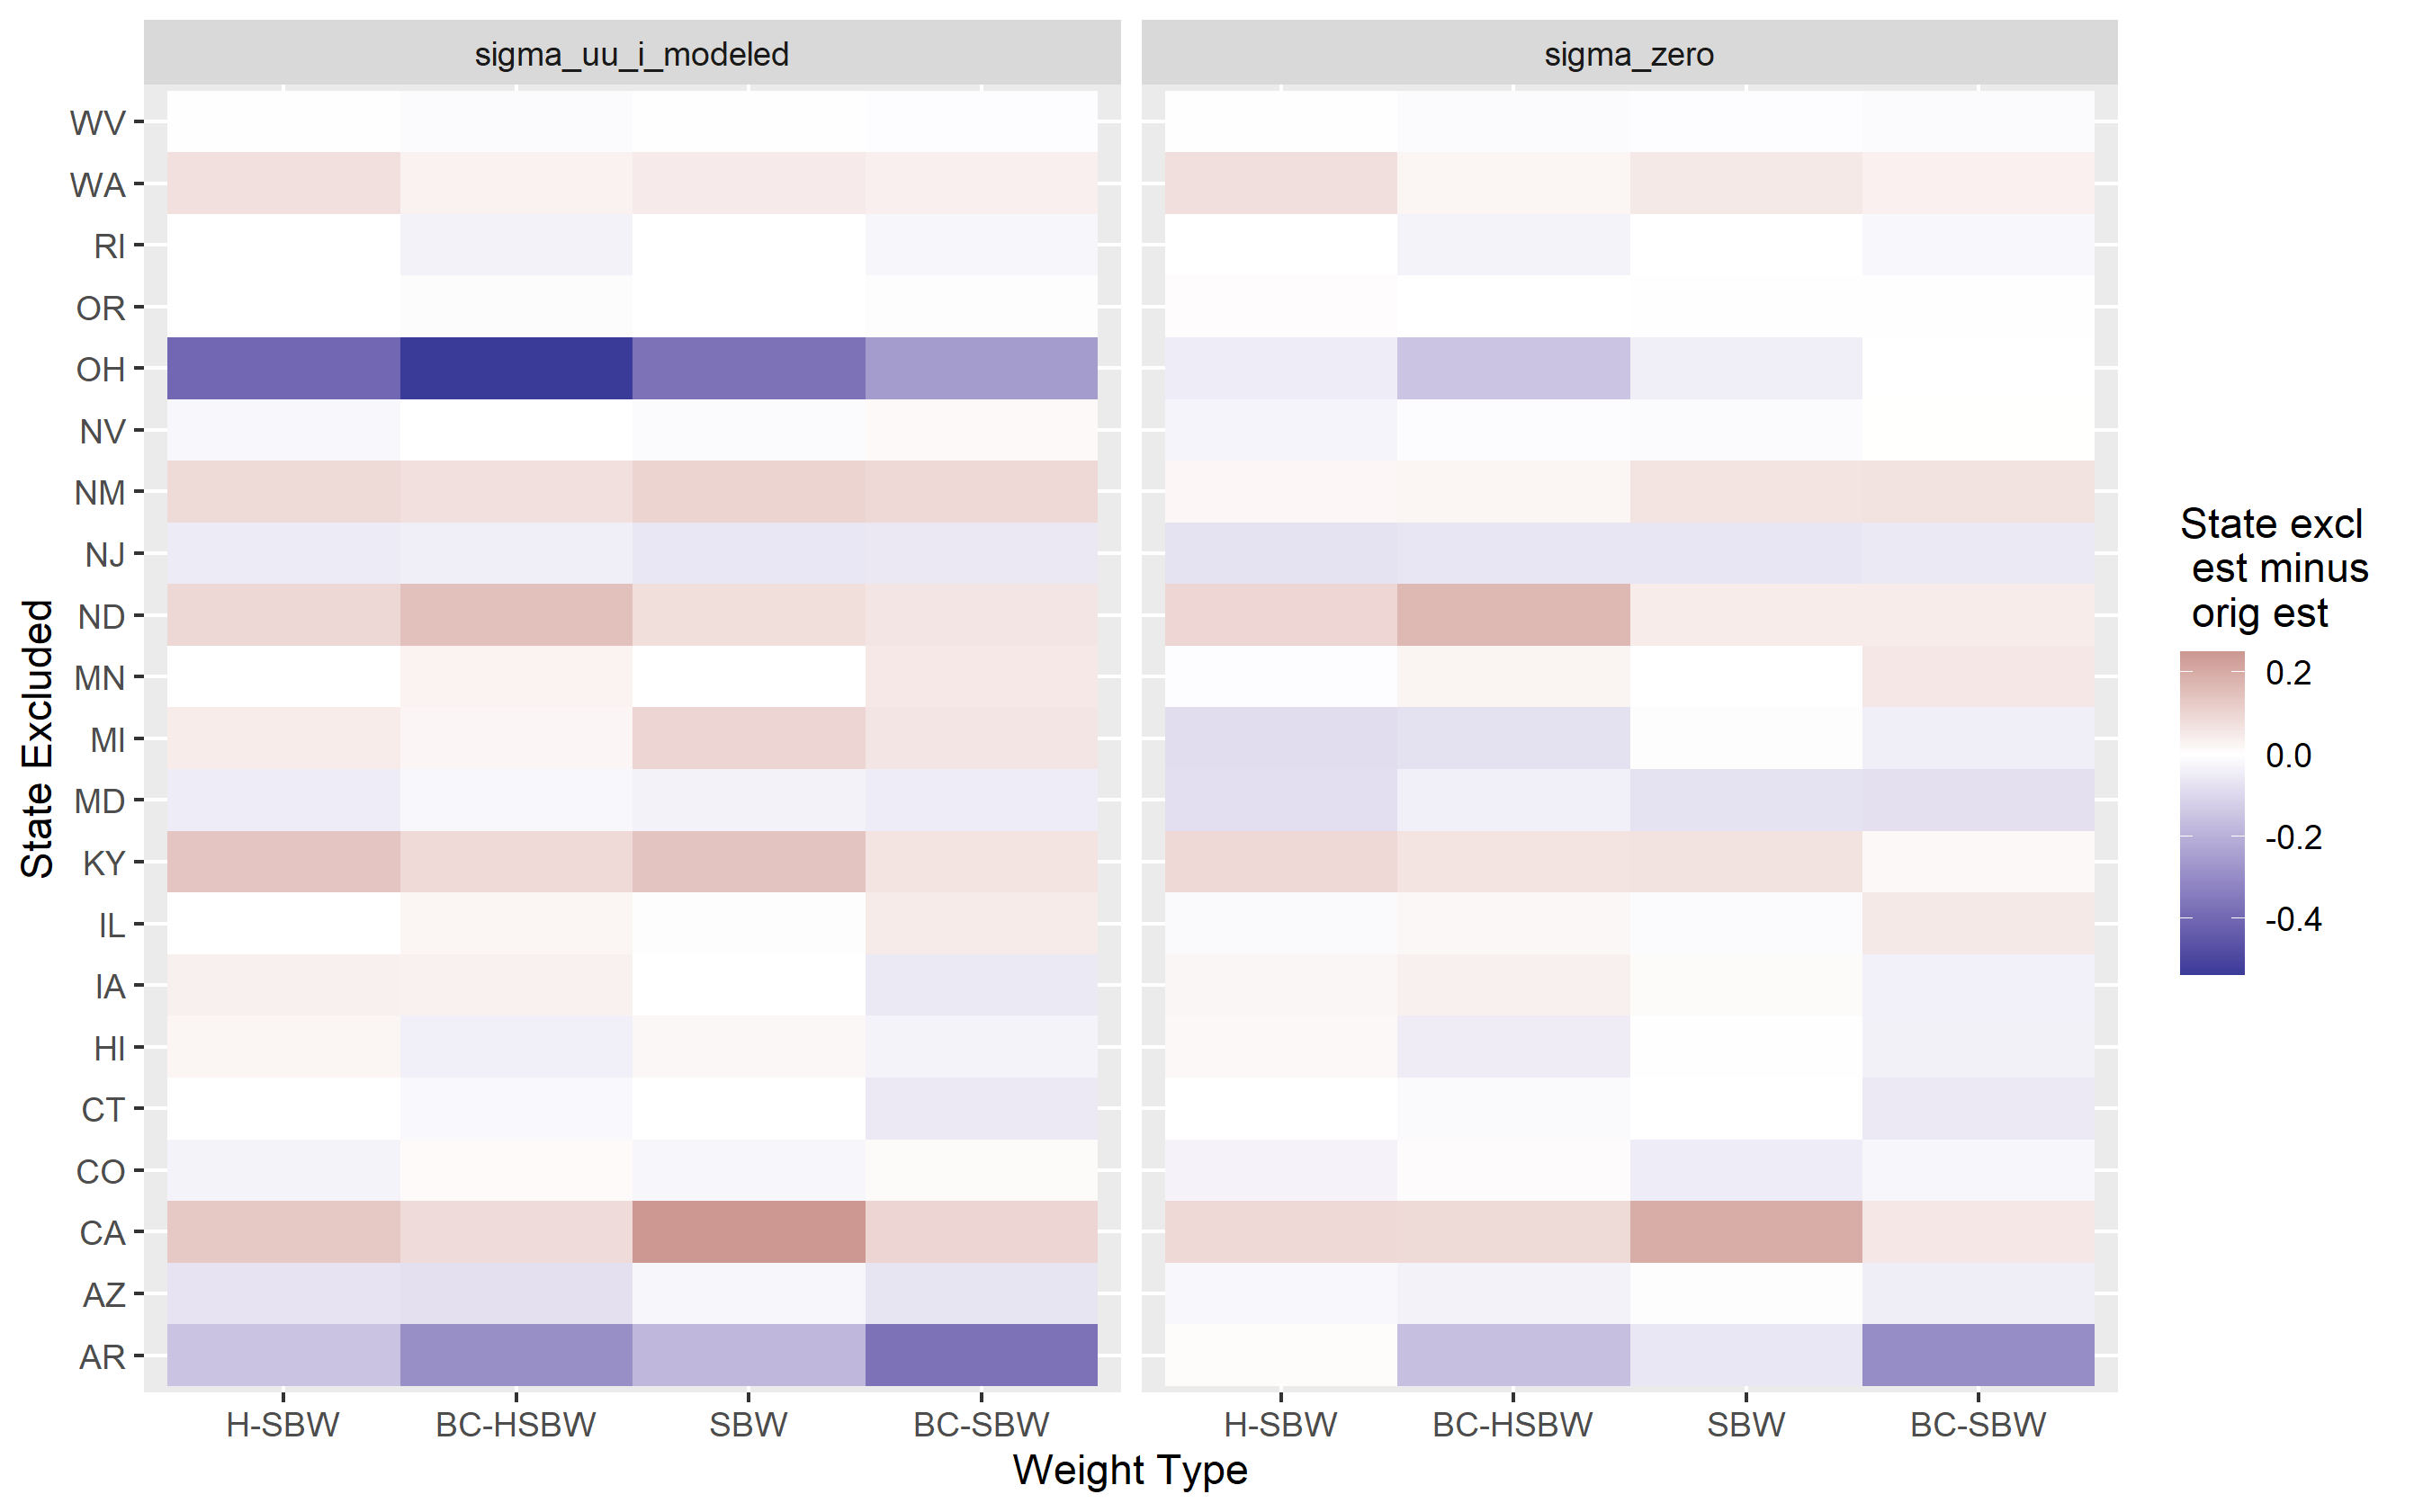
\includegraphics[scale=0.6]{01_Plots/loostate-sensitivityc1-state-uu-i.png}
\end{center}
\end{figure}

\subsection{Covariate importance}

We also investigate our hypothesis that factors associated with Governance are associated with treatment response. As discussed above, we first remove the balance constraints on the Republican governance indicators and estimate $\hat{\psi}^1_v$, and then subtract our original ETC point estimate from this quantity to generate $\hat{\Delta}_v^1$. Because this quantity does not reflect a clear population target, instead of confidence intervals, we present the minimum and maximum leave-one-state-out values in parentheses next to the original estimate.

For the H-SBW estimator we calculate $\hat{\Delta}^1$ equal to -0.69 (min = -0.83, max = -0.42) and equal to -0.79 (min = -0.90, max = -0.66) on our unadjusted dataset. In other words, our primary estimated treatment effect moved 0.78 percentage points further away from zero when we excluded the Republican governance indicators. This reflects a 33 percent decrease in our point estimate, a not-unsubstantial difference. Moreover, all of these estimates were less than zero, regardless of whether we conditioned on the covariate adjustment or not, regardless of whether we remove the early expansion states or not, and when removing each state. Across all specifications that we ran the minimum change we calculated was -1.34 and the maximum was -0.36. Additional distributional results across all leave-one-state-out estimates are available in Appendix E, Table~\ref{tab:rdiffc1}. Figure~\ref{fig:repub} displays our estimates of $\hat{\Delta}_v^1$ on our primary dataset and removing early expansion states (conditional on the covariate adjustment). 

We also consider four other covariate sets. We find that our estimates are most sensitive to controlling for pre-treatment outcomes and unemployment rates. This is not unexpected: all else equal, the expansion region had much lower pre-treatment uninsurance rates. If we do not control for these covariates, the comparable region will likely have lower pre-treament uninsurance rates, causing the estimated counterfactual to be closer to zero. The effect estimates were less sensitive to the removal of other covariate groups, and all point estimates are available in Appendix E, Table~\ref{tab:ptests}.

\begin{figure}[H]
\begin{center}
    \caption{Removing Republican Governance Indicators}
    \label{fig:repub}
    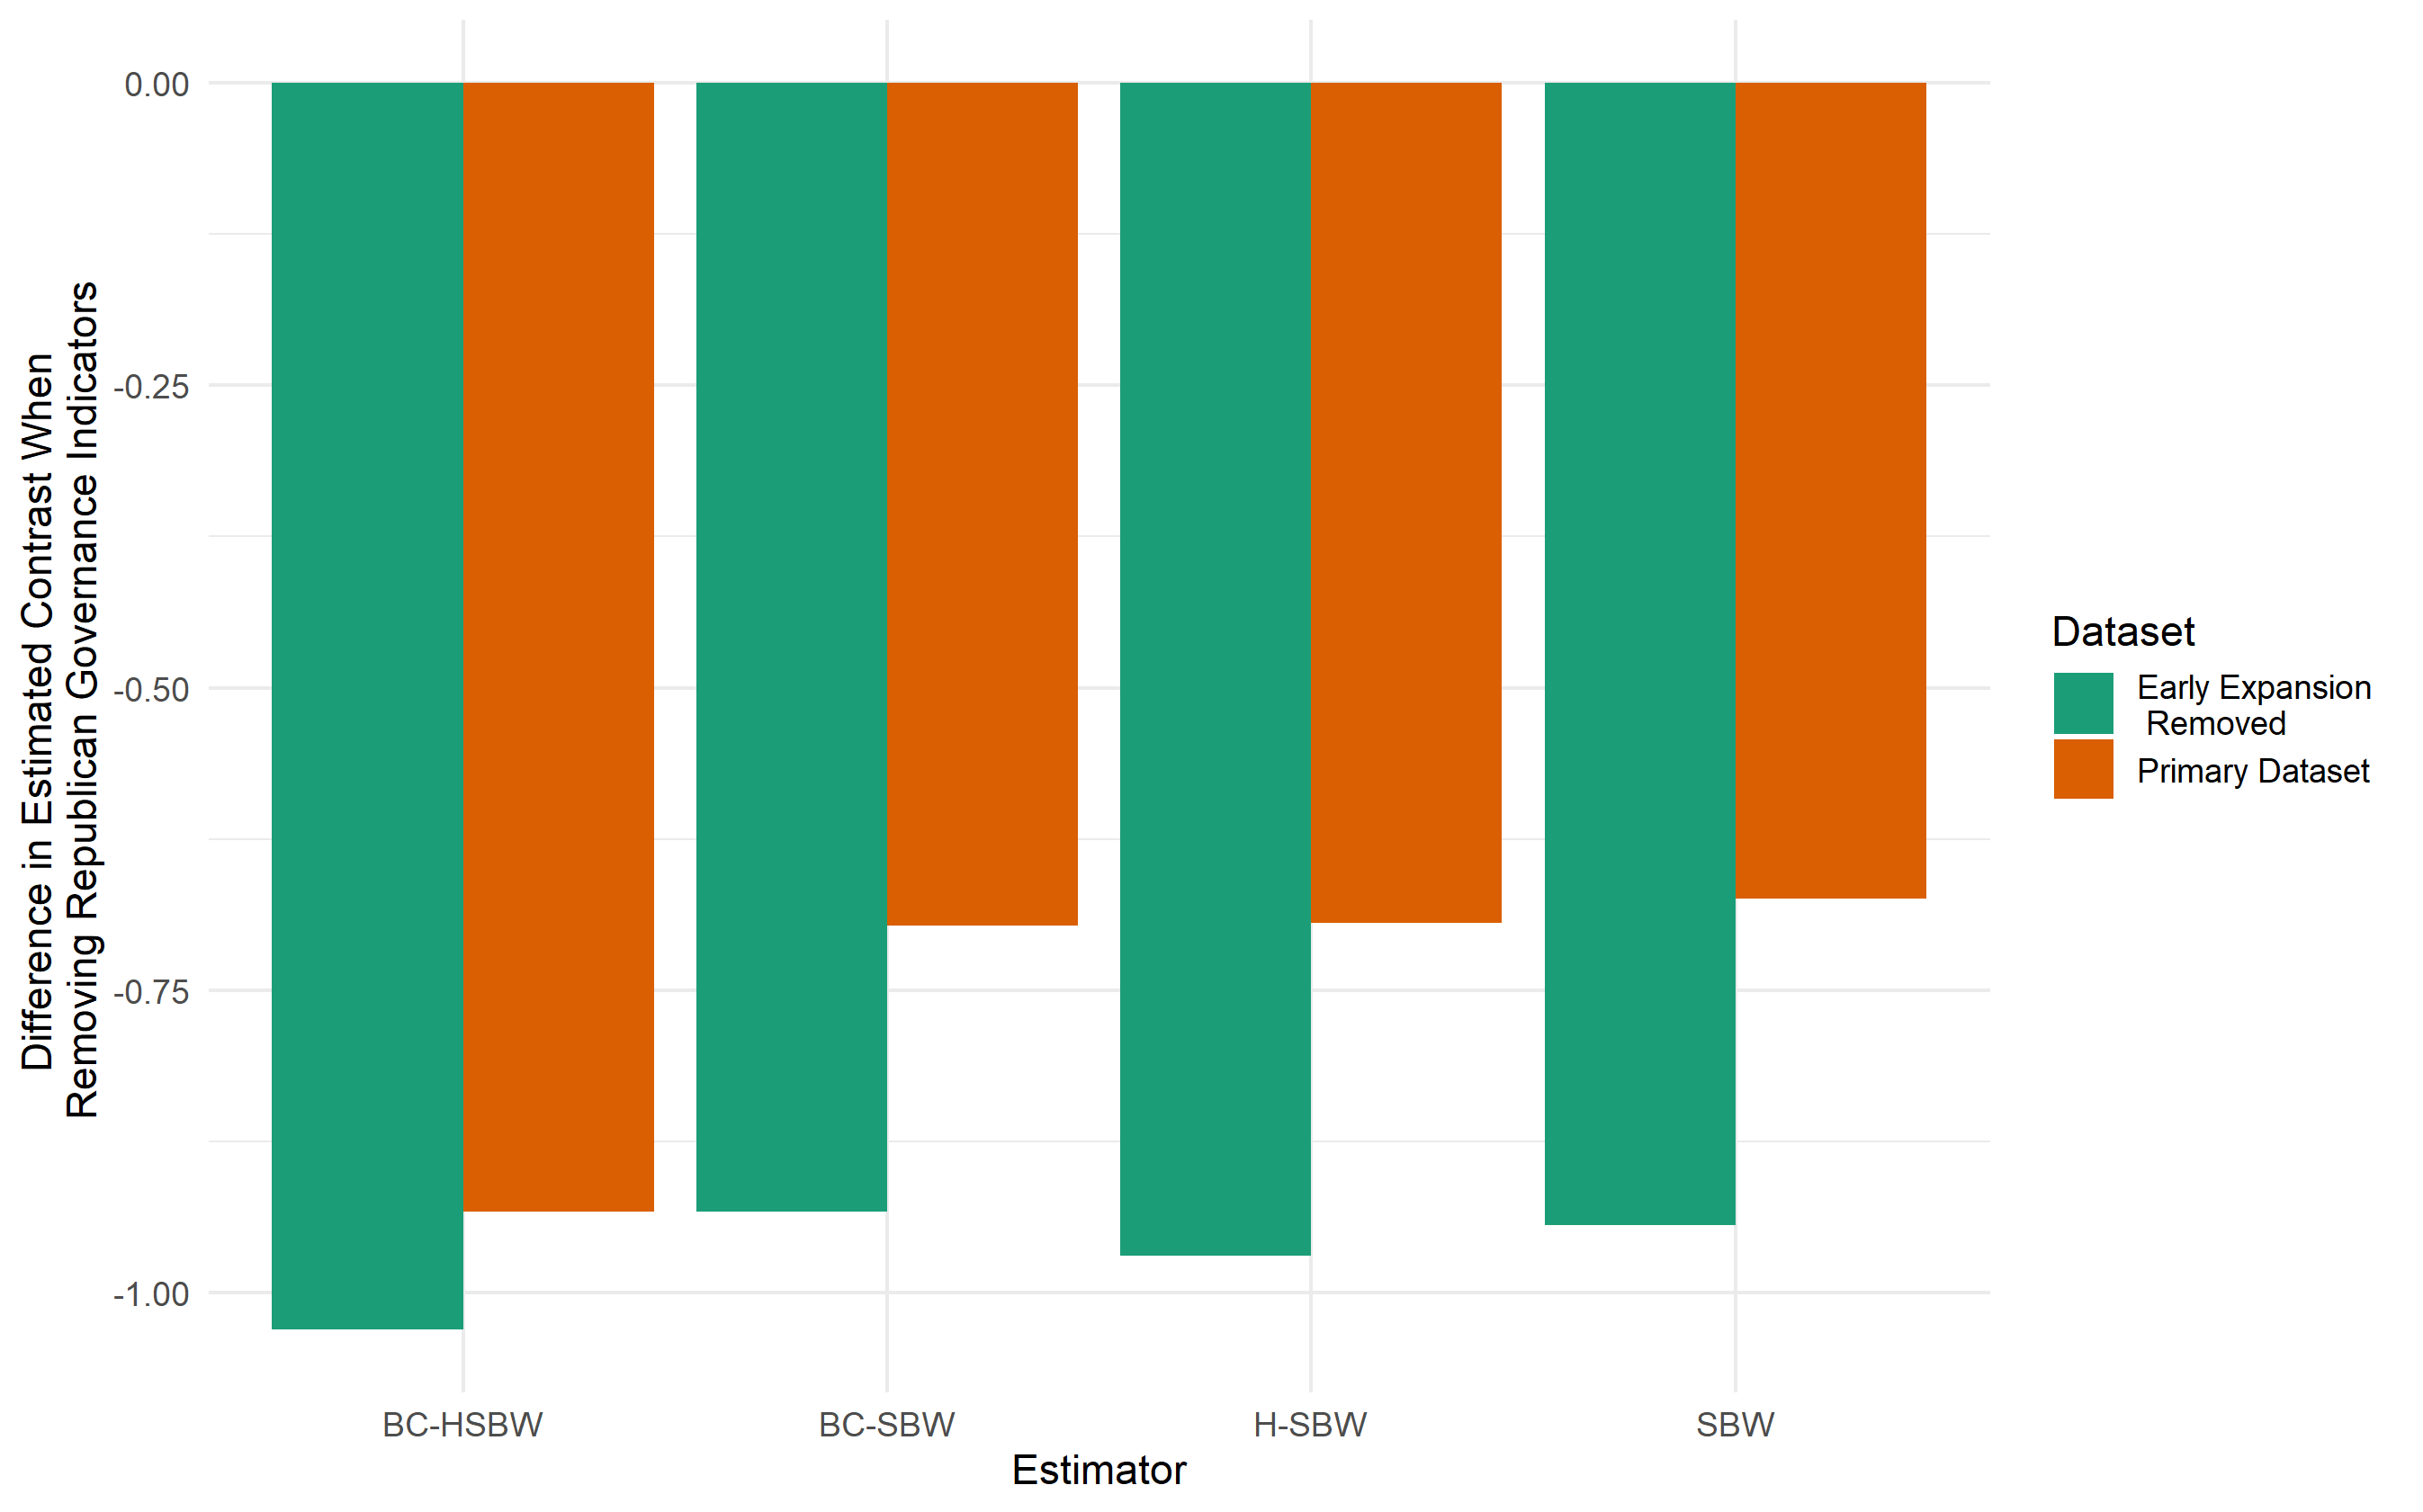
\includegraphics[scale=0.6]{01_Plots/repub-diff-all-estimators.png}
\end{center}
\end{figure}

These results highlight the importance of Republican governance in our counterfactual outcome model of $Y^1$. If the models specified by \cite{kaestner2017effects} and \cite{courtemanche2017early} are correct (that is, they correctly omit Republican governance from their balancing weights for estimating $\bar{Y}^0_{1, T}$), this would suggest treatment effect heterogeneity with respect to Republican governance. Moreover, because the expansion-state region is much more Democratic than the non-expansion region, this heterogeneity could potentially drive differences between the ETC and the ETT.

Since this is a policy question of some interest, we directly investigate this by estimating the outcome model on the full data with treatment assignment interacted with each covariate \footnote{For this analysis we calculate separate covariate adjustments on the untreated data. The summary statistics for this adjustment are available in Appendix D.}. We then examine how the estimated treatment effect would change if we decreased the interaction between treatment assignment and each Republican governance indicator -- Republican governor, Republican lower legislature control, and Republican total control -- by 50 percentage points (the original variables are either 0 or 100 and are measured at the state level). This linear combination of coefficients estimates how the treatment effect would change for any given collection of states against a set that is identical except for being 50 percentage points lower, on average, across the Republican governance indicators. We find that the linear combination is positive (0.21 percentage points) and statistically significant at the 5 percent level on the unadjusted dataset. In contrast to our previous results, this would indicate that the estimated treatment effect may be larger among Republican governed areas. However, this finding is not robust to any other specification that we run. Ultimately we interpret these results as providing no evidence of treatment effect heterogeneity with respect to Republican governance. The full results are available in Appendix E, Table~\ref{tab:hte}.



\section{Simulation Study}\label{app:simstudy}

This section presents a simulation study evaluating the performance of our proposed estimators on a known data-generating process. The first subsection outlines our simulation study. The section section presents selected results about the bias and mean-square error of our estimators, and the coverage rates for our proposed variance estimation procedure.

\subsection{Study design}

We first generate data according to a known and evaluate the performance of different estimators. For all models we consider the data generating process:

\begin{align*}
Y_{sc} \sim N(X_{1, sc} + X_{2, sc} + X_{3, sc}, \sigma^2_{\epsilon} + \sigma^2_{\varepsilon})
\end{align*}

where $\sigma^2_{\varepsilon}$ represents the variance component from a state-level random effect, and $\sigma^2_{\epsilon}$ represents a variance component from a CPUMA-level random effect. Thus the errors in the model for $Y \mid X$ are equicorrelated within state with correlation $\rho$ equal to $\frac{\sigma^2_{\varepsilon}}{\sigma^2_{\epsilon} + \sigma^2_{\varepsilon}}$

We next define a correlation structure among our observed covariates. Specifically, we generate each covariate vector $X_{sc}$:

\begin{align*}
X_{sc} \sim N(\mu_s, \Sigma_{Q}) \\
\mu_j \sim N(0, \Sigma_{S}) \\
\end{align*}

Define $\Sigma_X = \Sigma_Q + \Sigma_S$. Let $\sigma^2_{x, j}$ be the j-th diagonal element of $\Sigma_X$ (and define $\sigma^2_{q, j}$ and $\sigma^2_{s, j}$ analogously). Across all simulations, we fix $\sigma^2_{x, j} = 2$. We also fix the off-diagonal elements of both $\Sigma_Q$ and $\Sigma_S$ to be equal and so that $Cor(X_j, X_k) = 0.25$. Finally, define $\rho_x = Cor(X_{sc}, X_{sd})$ for $c \ne d$; in other words, $\rho_x$ is the within-state correlation of the covariates $X_{sc}$, which we set to be equal for all covariates.

We also consider samples of size $m = 25$ states each with $p_s$ units and $n$ total units. We draw $p_s \stackrel{iid}\sim \lfloor Exp(0.1) + 10\rfloor$ so that the average number of regions per state is approximately 20 (and the approximate number of total units $n$ is on average approximately 450).

We next generate our noisy outcome and covariate estimates $(J, W)$:

\begin{align*}
(J_{sc}, W_{sc}) \stackrel{iid}\sim N((Y_{sc}, X_{sc}), \Sigma_{\nu, sc})
\end{align*}

\begin{align*}
    \Sigma_{\nu} = \begin{pmatrix}
    \sigma^2_{\nu, sc} & 0 & 0 & 0 \\
    0 & \sigma^2_{\nu, sc} & 0 & 0 \\
    0 & 0 & \sigma^2_{\nu, sc} & 0 \\
    0 & 0 & 0 & \sigma^2_{\nu, sc}
    \end{pmatrix}
\end{align*}

First, define $\rho_y = \sigma^2_{\varepsilon}/(\sigma^2_{\epsilon} + \sigma^2_{\varepsilon} + \sigma^2_{\nu})$. In other words, $\rho_y$ represents the within-state correlation of the outcome model errors, including the measurement errors in the outcome. We fix this to be 0.25 throughout all simulations.

We allow $\sigma^2_{\nu, sc}$ to be a function of the sample size of an underlying survey that generates the estimate. We simulate these sample sizes $r_{sc}$ drawn from some distribution (see more on this below). Let $R_{sc}$ be a 3x3 diagonal matrix with diagonal elements $r_{sc}$. Let $\sigma_{\nu}^{2\star}$ be defined as the limit as $n \to \infty$ of $n^{-1}\sum_{sc}\sigma^2_{\nu, sc}$ (we ensure this limit exists). Let $\tau = \sigma^2_x/\sigma^2_w$. We then fix a value $\sigma_{\nu}^{2\star}$ so that that as $n \to \infty$, $n^{-1} \tau \sum_{sc}\frac{\sigma^2_{\nu}}{r_{sc}} \to^p \sigma^2_{\nu}$. In other words, $\sigma_{\nu}^2$ represents the common variance that generate all errors in the ``heterogeneous adjustment'' model. We also simulate homoskedastic measurement errors, letting $\sigma^2_{\nu, sc} = \sigma^2_{\nu}$. 

For our simulations we generate population datasets of $m = 5000$ that consider all XX combinations of the following parameters:

\begin{itemize}
    \item $(r_{sc} \sim Unif(300, 2300), r_{sc} = 1)$ 
    \item $\rho_x \in \{0, 0.25, 0.5\}$
    \item $\tau \in \{0.95, 0.9, 0.85\}$
\end{itemize}

For each parameterization we take 500 random samples of size $m = 25$ and estimate H-SBW weights with targeting $\upsilon_0 = c(1, 1, 1)$. We set $\delta = 0$ and consider $\rho \in \{0, 0.25, 0.5\}$. We then estimate weights that reweight the following datasets to $\upsilon_0$: ($W_{A=1}$, $X_{A=1}$, $\tilde{X}_{A=1}^{hom}$, $\tilde{X}_{A=1}^{hom}$, $\tilde{X}_{A=1}^{cor}$), as defined in Appendix~\ref{app:adjustmentdetails}. We estimate the variance for each estimator using the leave-one-state-out jackknife, described in Section~\ref{sec:methods}.
 
Note: for $\hat{\kappa}$ we use the empirical covariance matrix of $W$, the estimated means $\bar{W}$, and $\hat{\Sigma}_{\nu, sc}$, where we draw $\hat{\Sigma}_{\nu, sc}$ from $\Sigma_{\nu, sc} + N(0, 0.001*n*I_d)$. In other words, when averaged together we assume that $\hat{\Sigma}_{\nu}$ have a fairly precise estimate of $\Sigma_{\nu}$.

\subsection{Selected results}

We present selected results from this study. We consider where the measurement error variances are heterogeneous (i.e. the ``heterogeneous adjustment'' model is correct). Figure~\ref{fig:simbias} displays the bias associated with each estimator. From left to right, the panels reflect different values of $\tau = \sigma^2_x/\sigma^2_w$ -- the left-most panels have the most measurement error while the right-most panels have the least. From top to bottom the panels reflect different values of $\rho_x$: the top-most panel has no correlation structure among the covariates, while the bottom-most panels are more highly correlated within state. Within each panel we organize each result by which covariate set was balanced: $W$ represents the estimators generated without any covariate adjustment; $X$ reflects estimators generated on the true covariates; ``Xhat-het'' ($\hat{X}_{A=1}^{het}$) represents the heterogeneous adjustment, ``Xhat-hom'' ($\hat{X}_{A=1}^{hom}$) represents the homogeneous adjustment, and ``Xhat-cor'' ($\hat{X}_{A=1}^{cor}$) represents the correlated adjustment. The estimators are colored by the assumed value of $\rho$ in the H-SBW objective: across all simulations, the true correlation for the outcome model ($\rho_y$) is again 0.25.

We highlight a few interesting results. First, if we know the true values of $X$, we see that all of our estimators are unbiased estimate. However, we see that balancing on $W$ results in bias, and the bias increases as $\tau$ decreases. Third, setting $\rho > 0$ exacerbates this bias: this aligns with our expectations from Remark~\ref{rmk:glsbias}, when we considered GLS weights in the context of measurement error.

We then try to mitigate this bias by using some estimate of $\mathbb{E}[X \mid W, A]$. We see that when the covariates  uncorrelated (i.e. the top set of panels), balancing on $X$, $\hat{X}_{A=1}^{hom}$, $\hat{X}_{A=1}^{het}$, or $\hat{X}_{A=1}^{cor}$ results in approximately unbiased estimates for all values of $\rho$. This aligns with our theoretic results in Appendix~\ref{app:AsecI}. However, we also see that when $X$ are correlated, setting $\rho > 0$ results in biased estimates for $\hat{X}_{A=1}^{het}$ or $\hat{X}_{A=1}^{hom}$; however, we still obtain approximately unbaised estimates for $\rho = 0$ (SBW). Even so the bias from H-SBW is still much less than the bias for the corresponding estimates that balance on $W$ when using $\hat{X}_{A=1}^{het}$ or $\hat{X}_{A=1}^{hom}$.

Interestingly, our proposed adjustment to asymptotically remove the bias from H-SBW -- $\hat{X}_{A=1}^{cor}$ -- appears to make this bias worse given the sample size considered here. In Section~\ref{appssec:simstudyresults2}, we show results verifying that this procedure is consistent as we increase $m$.

\begin{figure}[H]
\begin{center}
    \caption{Simulation study: estimator bias}\label{fig:simbias}
    \label{fig:loveplotc1}
    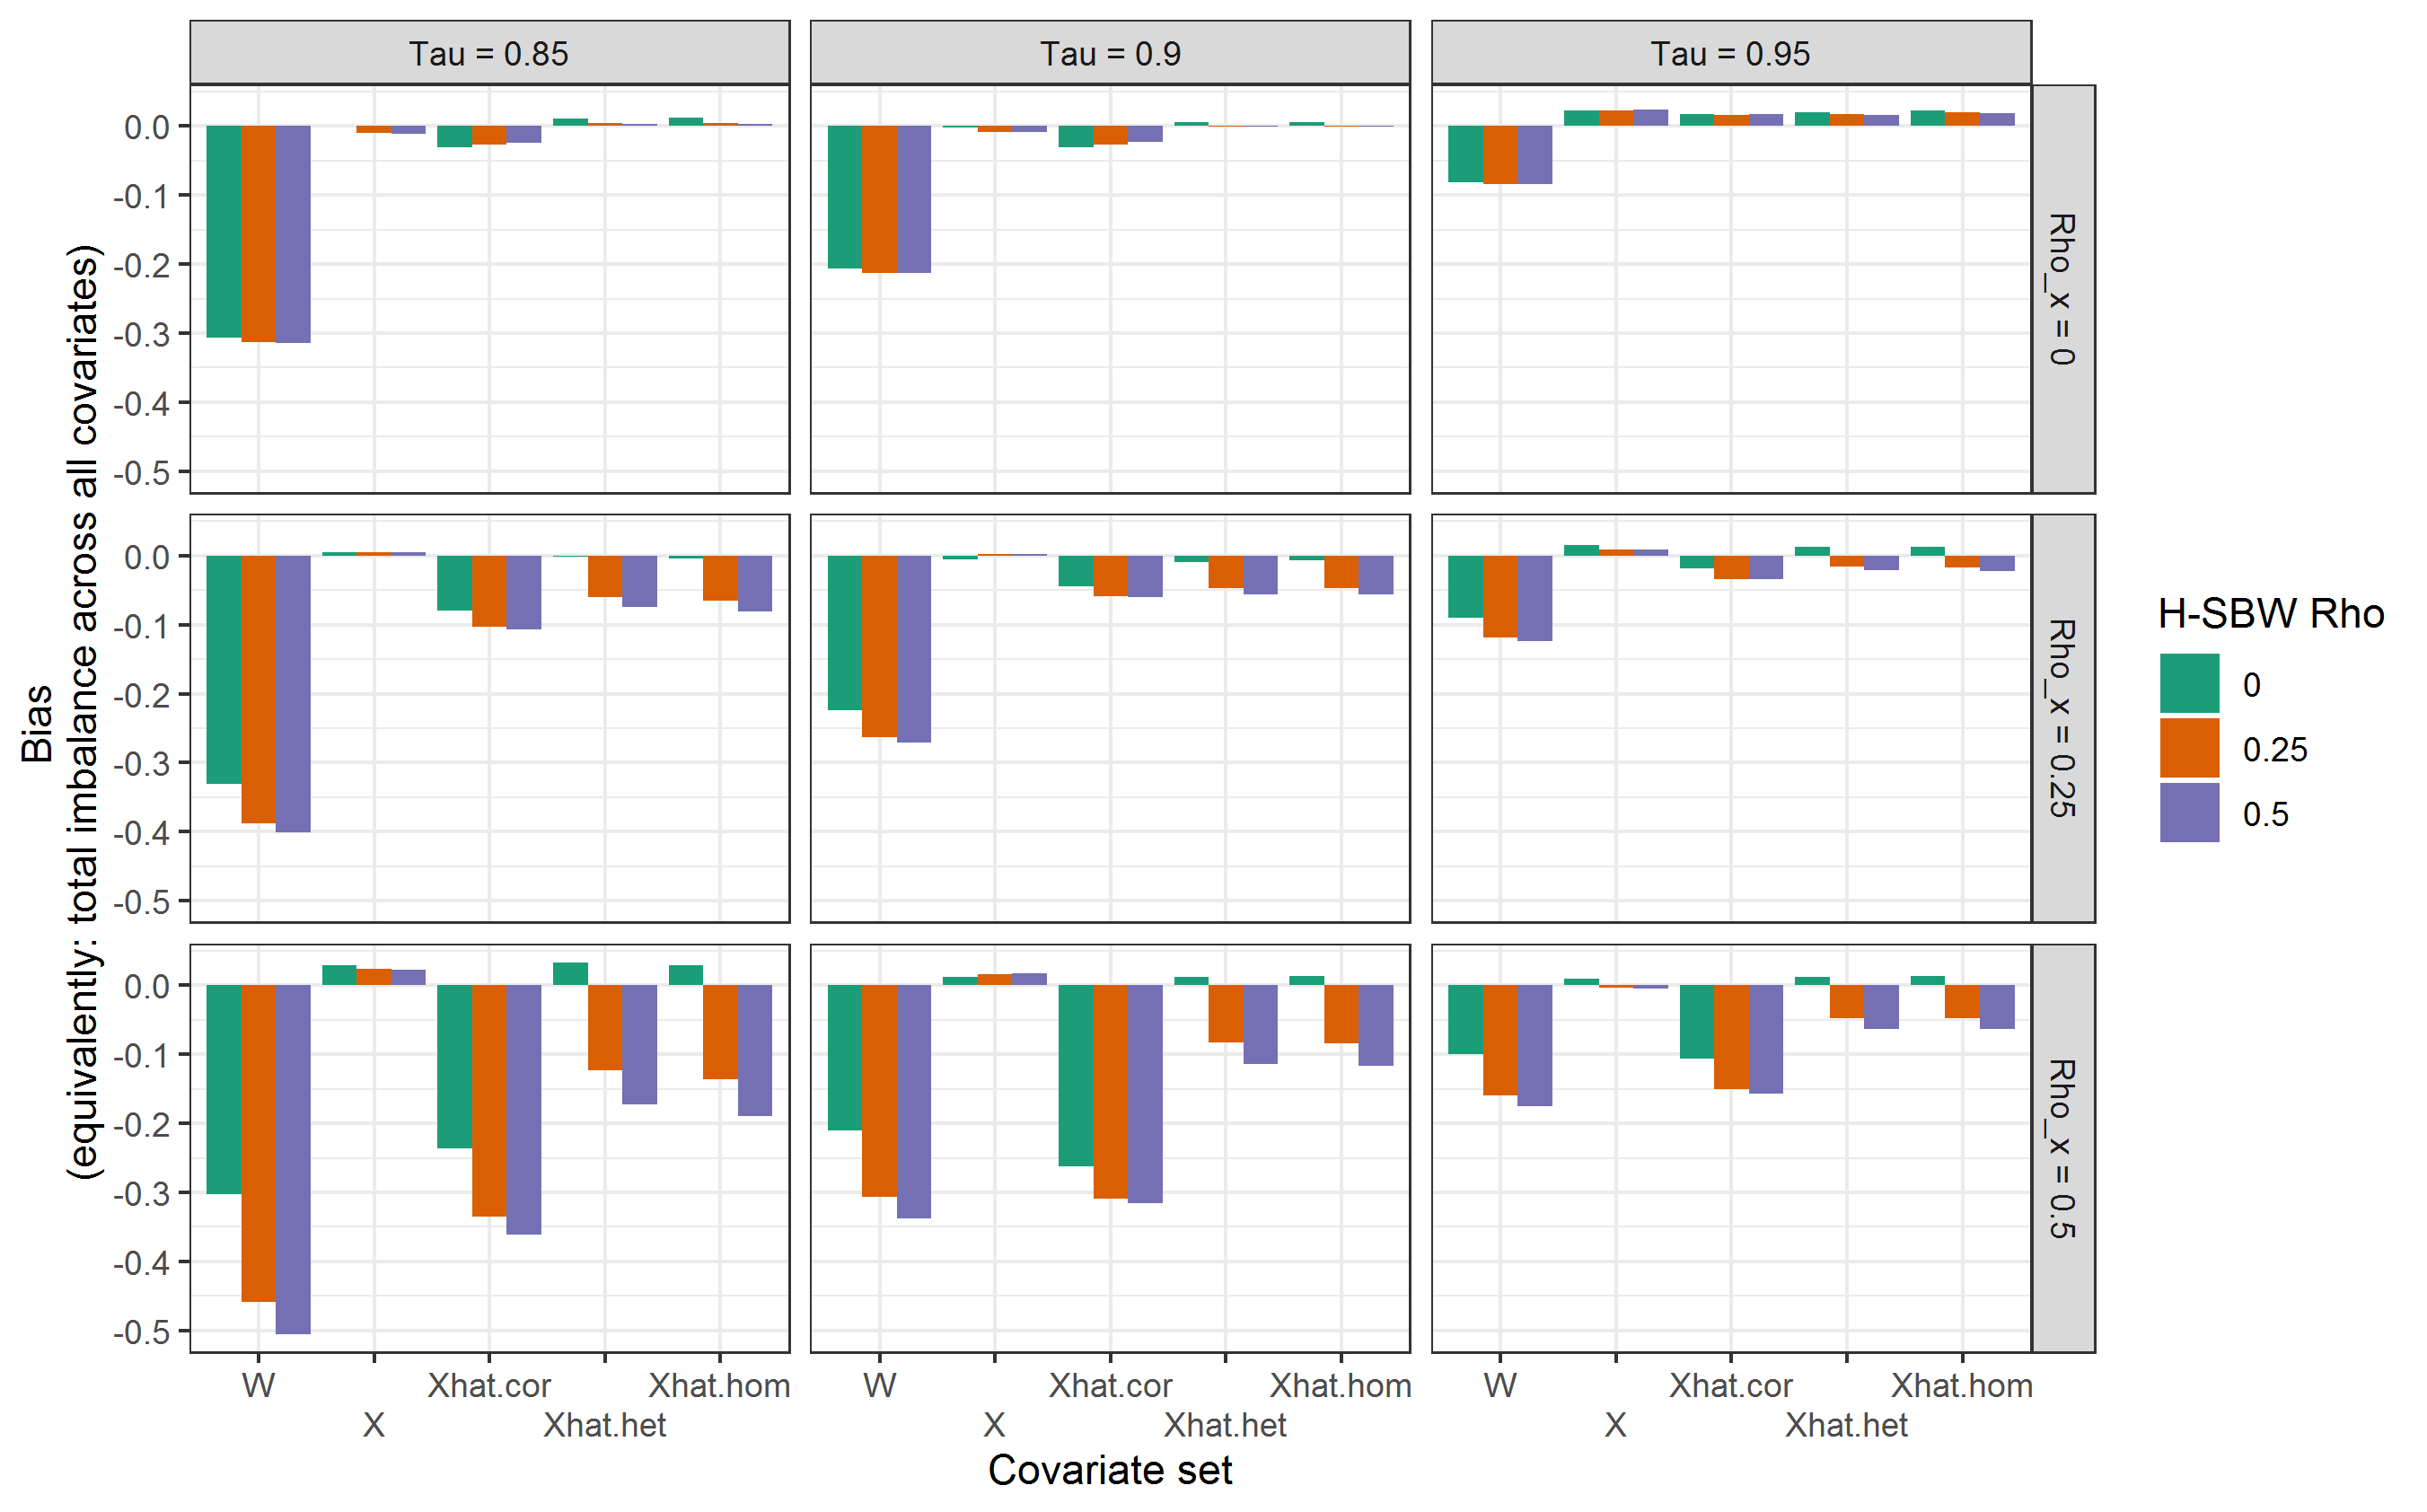
\includegraphics[scale=0.5]{01_Plots/bias-plot.png}
    \subcaption{Averaged across 500 simulations for each specification}
\end{center}
\end{figure}

All of these simulations had heterogeneous measurement. When we examine the results when the errors are homogeneous (results not displayed but available on request), we find that the estimators that balance on $\tilde{X}^{het}_{A=1}$ have a small bias even when $\tau = 0$ or $\rho = 0$. Assuming this model is correct when it is not appears to have some cost. This may help explain the worse performance we found when applying the heterogeneous adjustment to our validation study in Section~\ref{sec:results}.

We next calculate the variance our estimates across all simulations and display these results in Figure~\ref{fig:simvar}. Unsurprisingly, we find that we obtain a modest variance reduction as we increase $\rho$. Interestingly, even when $\rho$ is incorrect (assumed $0.5$ instead of $0.25$), we tend to get nearly identical improvements to $\rho = 0.25$. We also see that balancing on $\tilde{X}^{cor}_{A=1}$ can lead to a much more variable estimate, again suggesting a large cost to using this procedure given a small sample size.

\begin{figure}[H]
\begin{center}
    \caption{Simulation study: estimator variance}\label{fig:simvar}
    \label{fig:loveplotc1}
    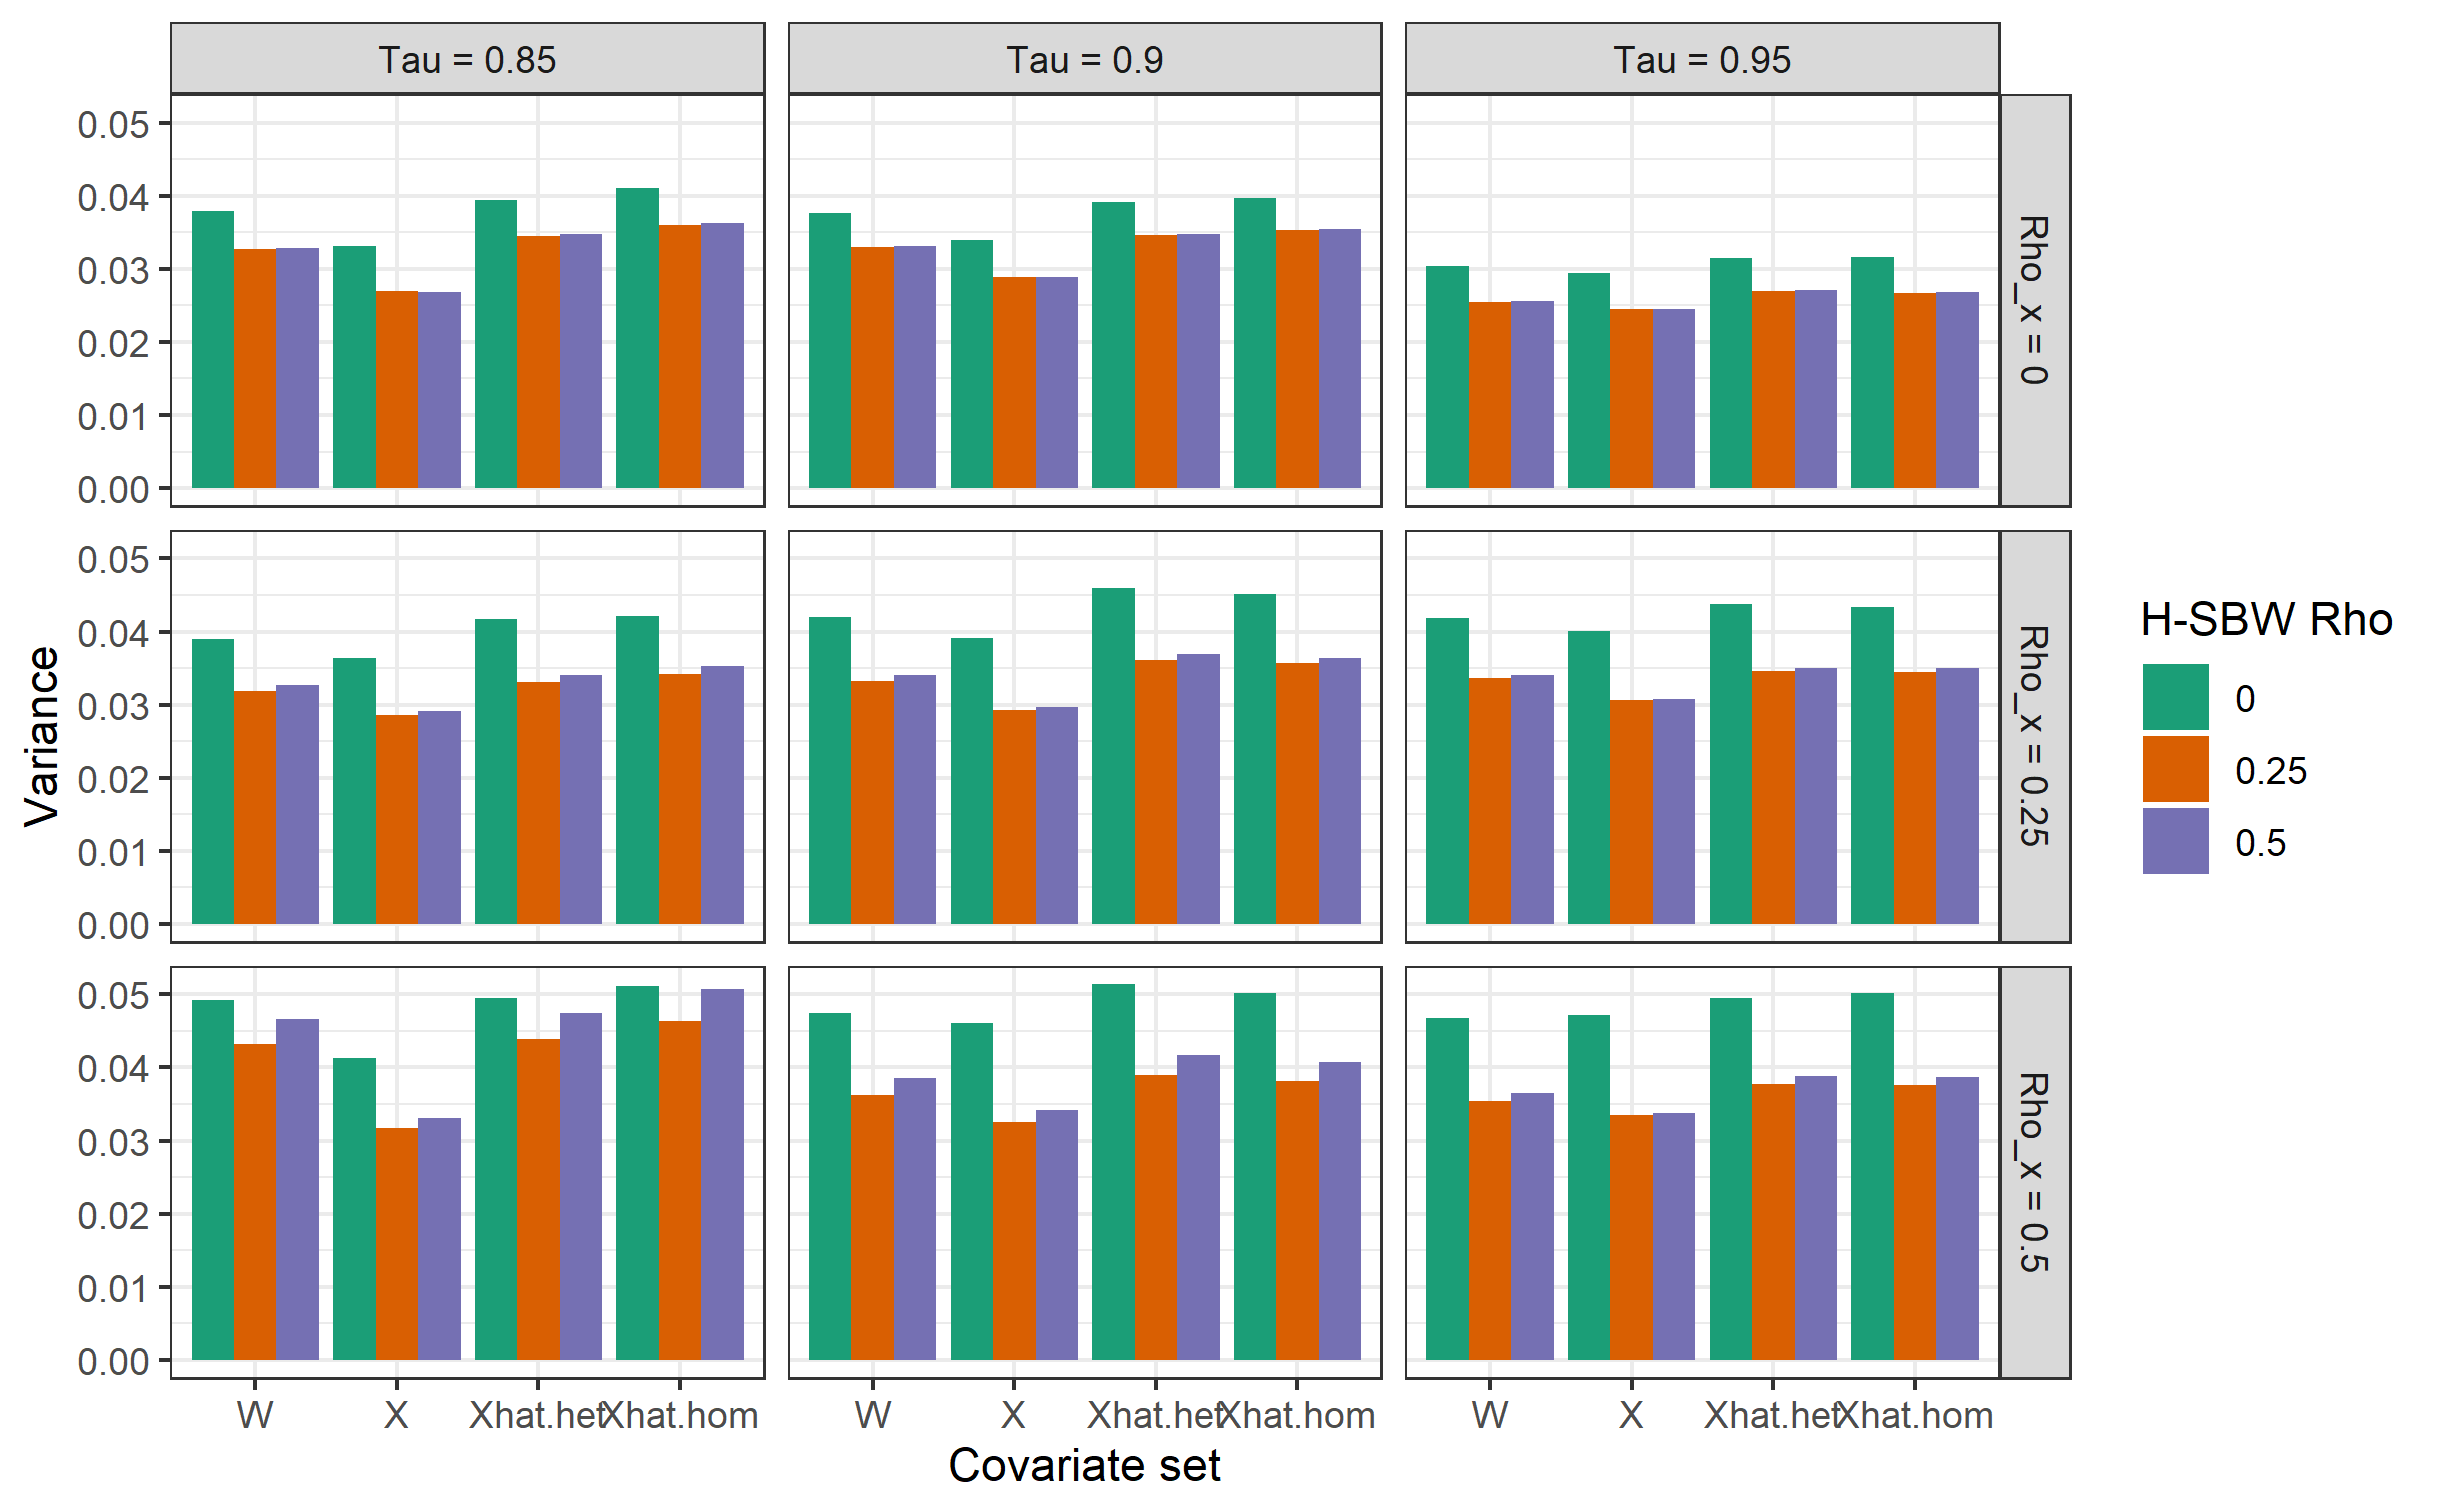
\includegraphics[scale=0.5]{01_Plots/var-plot.png}
    \subcaption{Averaged across 500 simulations for each specification}
\end{center}
\end{figure}

In Figure~\ref{fig:simmse} we display the MSE of these estimators (we remove $\tilde{X}_{A=1}^{cor}$ since we have already seen that it has poor performance relative to the other procedures considered). We find that despite the increase in bias for H-SBW with $\hat{X}_{A=1}^{hom}$ or $\hat{X}_{A=1}^{het}$, we may still find a modest MSE reduction. In particular, we see that this is more likely in regimes with low measurement error and less correlated covariates. Of course, more generally this also depends on $\rho_y$, which we have fixed here throughout: if we were to set $\rho_y = 0$, we would expect the MSE of these estimators to increase for all estimators as $\rho$ increased, even when we observe $X$. 

\begin{figure}[H]
\begin{center}
    \caption{Simulation study: estimator mean-square-error}\label{fig:simmse}
    \label{fig:loveplotc1}
    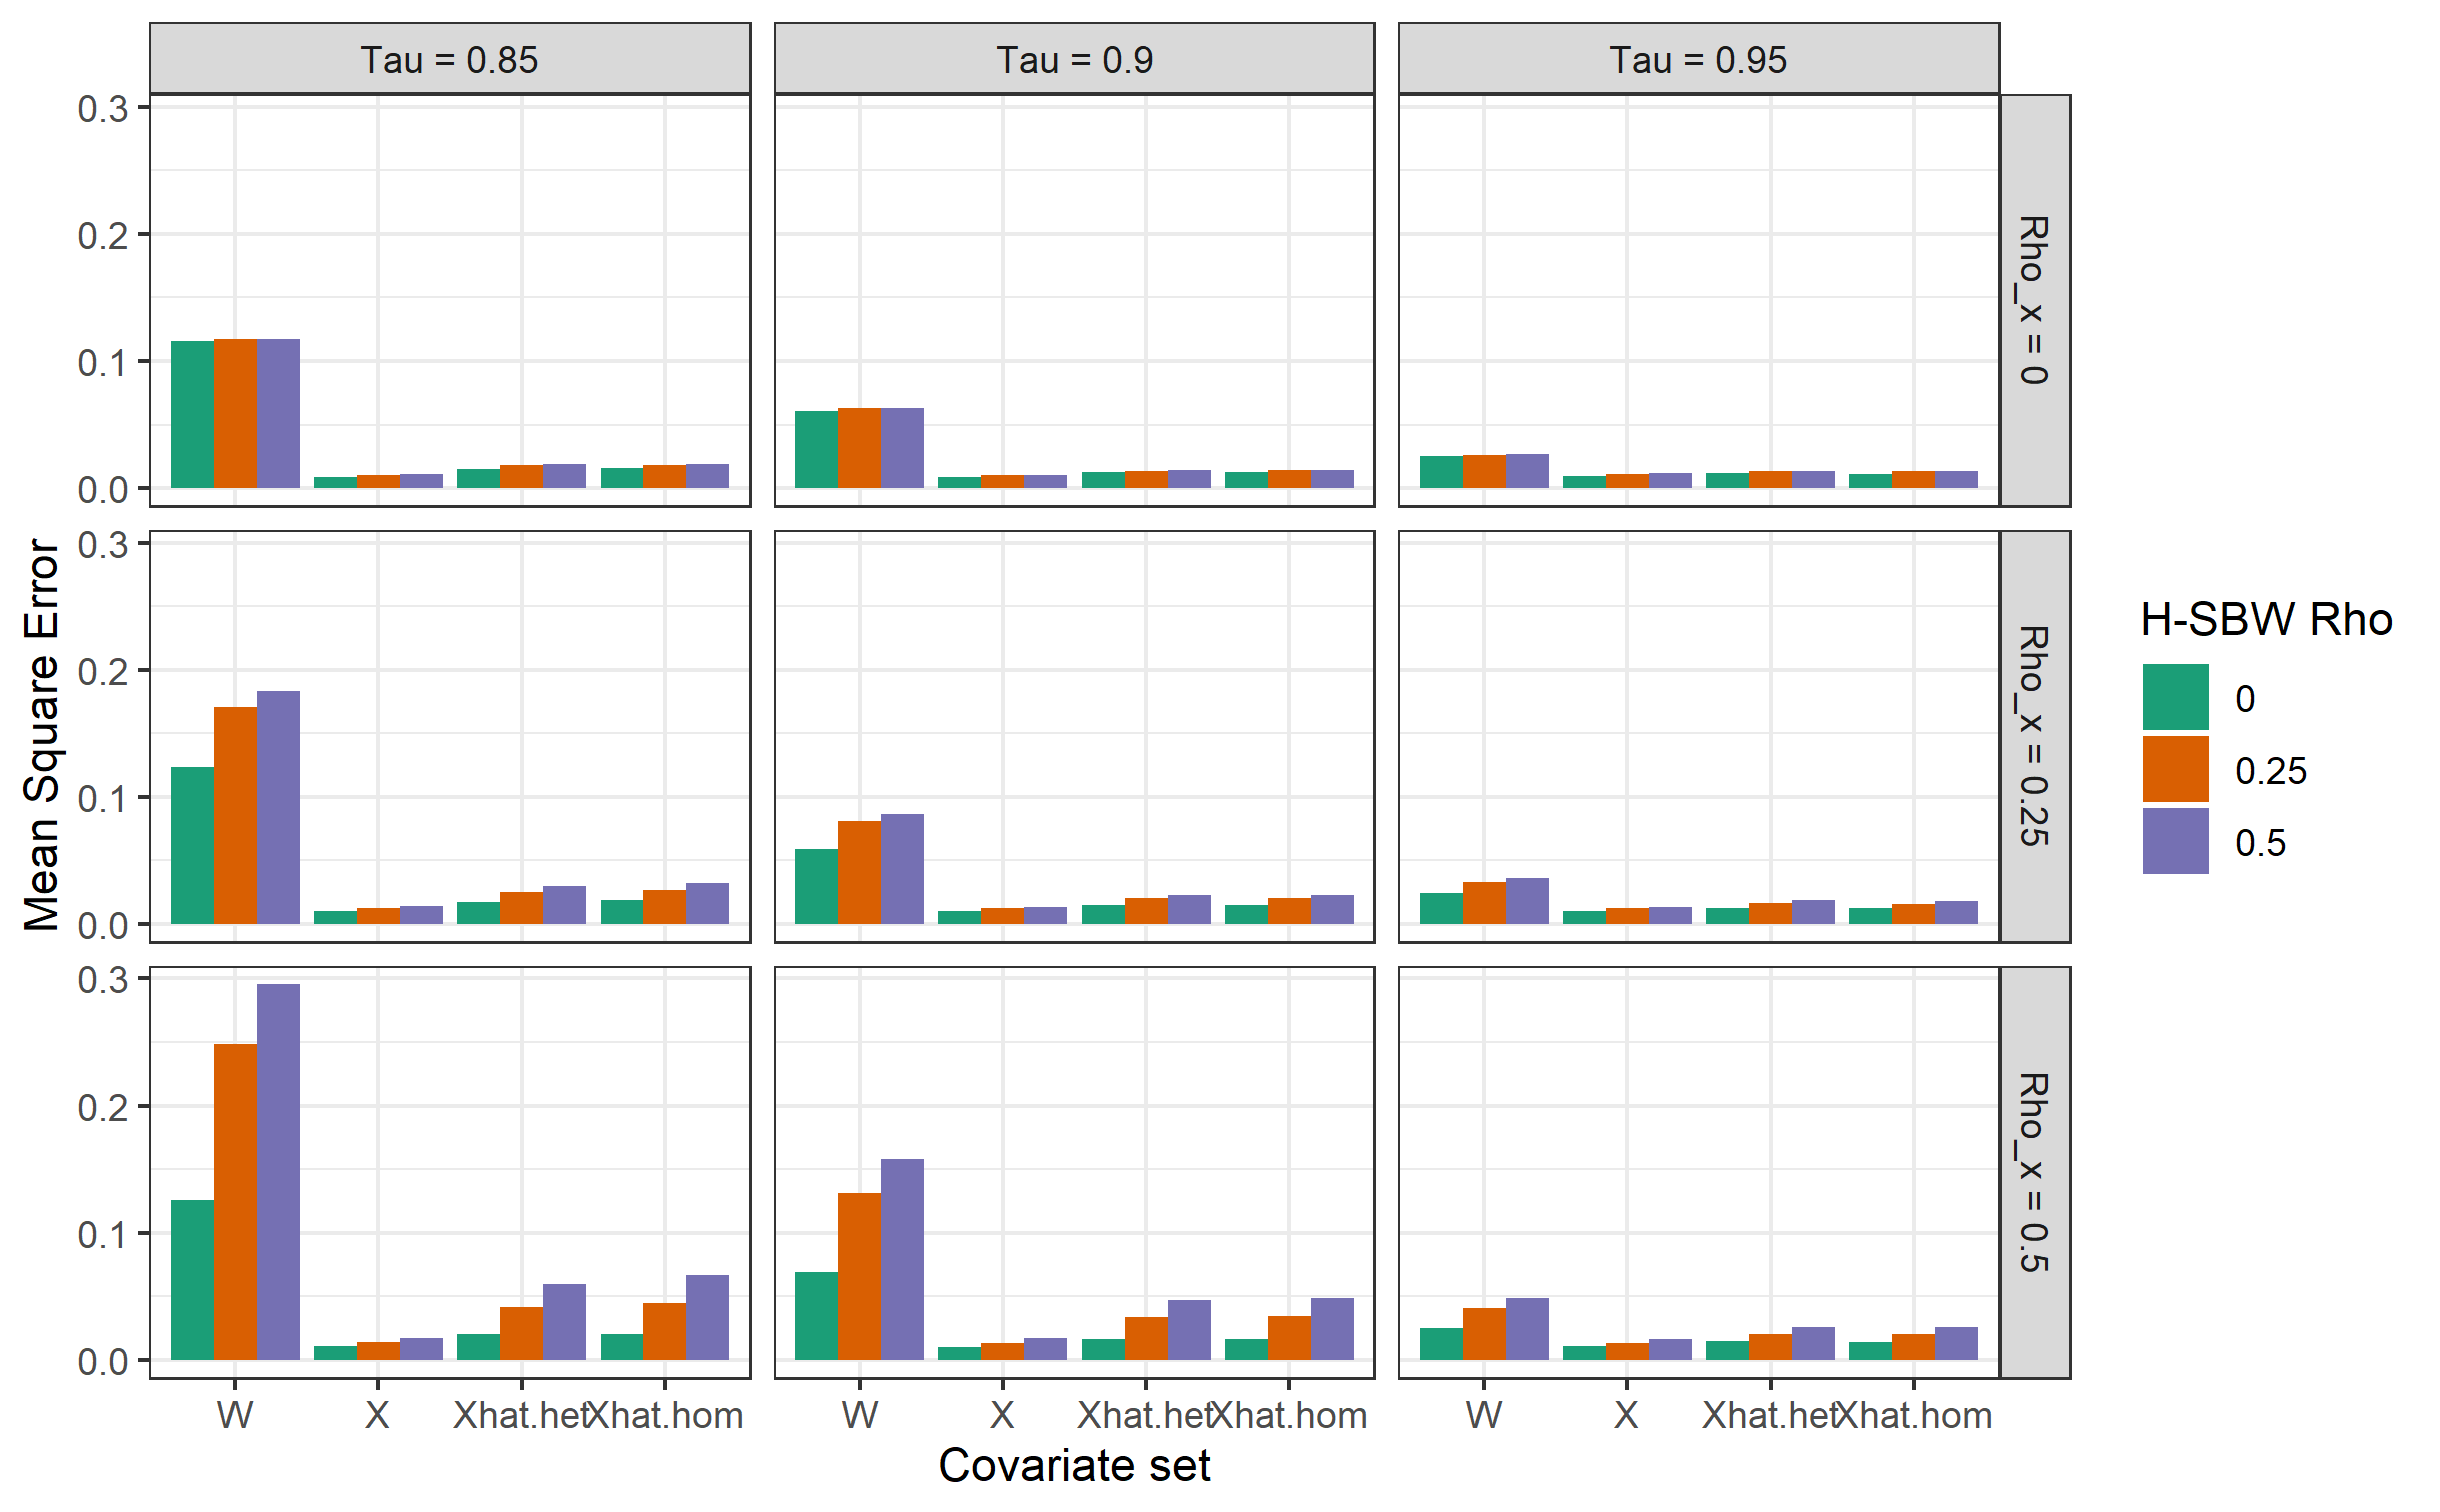
\includegraphics[scale=0.5]{01_Plots/mse-plot.png}
    \subcaption{Averaged across 500 simulations for each specification}
\end{center}
\end{figure}

Finally, we evaluate the performance of the leave-one-state-out jackknife procedure and evaluate confidence interval coverage and length. We display these results in Figures~\ref{fig:simcoverage1} and ~\ref{fig:simcoverage2}. 

We first discuss Figure~\ref{fig:simcoverage1}. When $\rho = 0$ we find that we obtain approximately nominal coverage rates across all specifications that use $X$ or some version of $\hat{X}$. However, we fail to get even close to nominal coverage rates when balancing on $W$, even when $\tau$ is quite high. We do see the performance of our estimates deteriorate as we increase $\rho_x$, even when balancing on the true covariates. We also see that our coverage rates tend to get worse for $\hat{X}^{het}$ and $\hat{X}^{hom}$ in the settings where we found the highest bias. On the other hand, we also find that our coverage rates are often quite conservative, particularly for estimators generated on $\hat{X}$. 

\begin{figure}[H]
\begin{center}
    \caption{Simulation study: jackknife coverage rates}\label{fig:simcoverage1}
    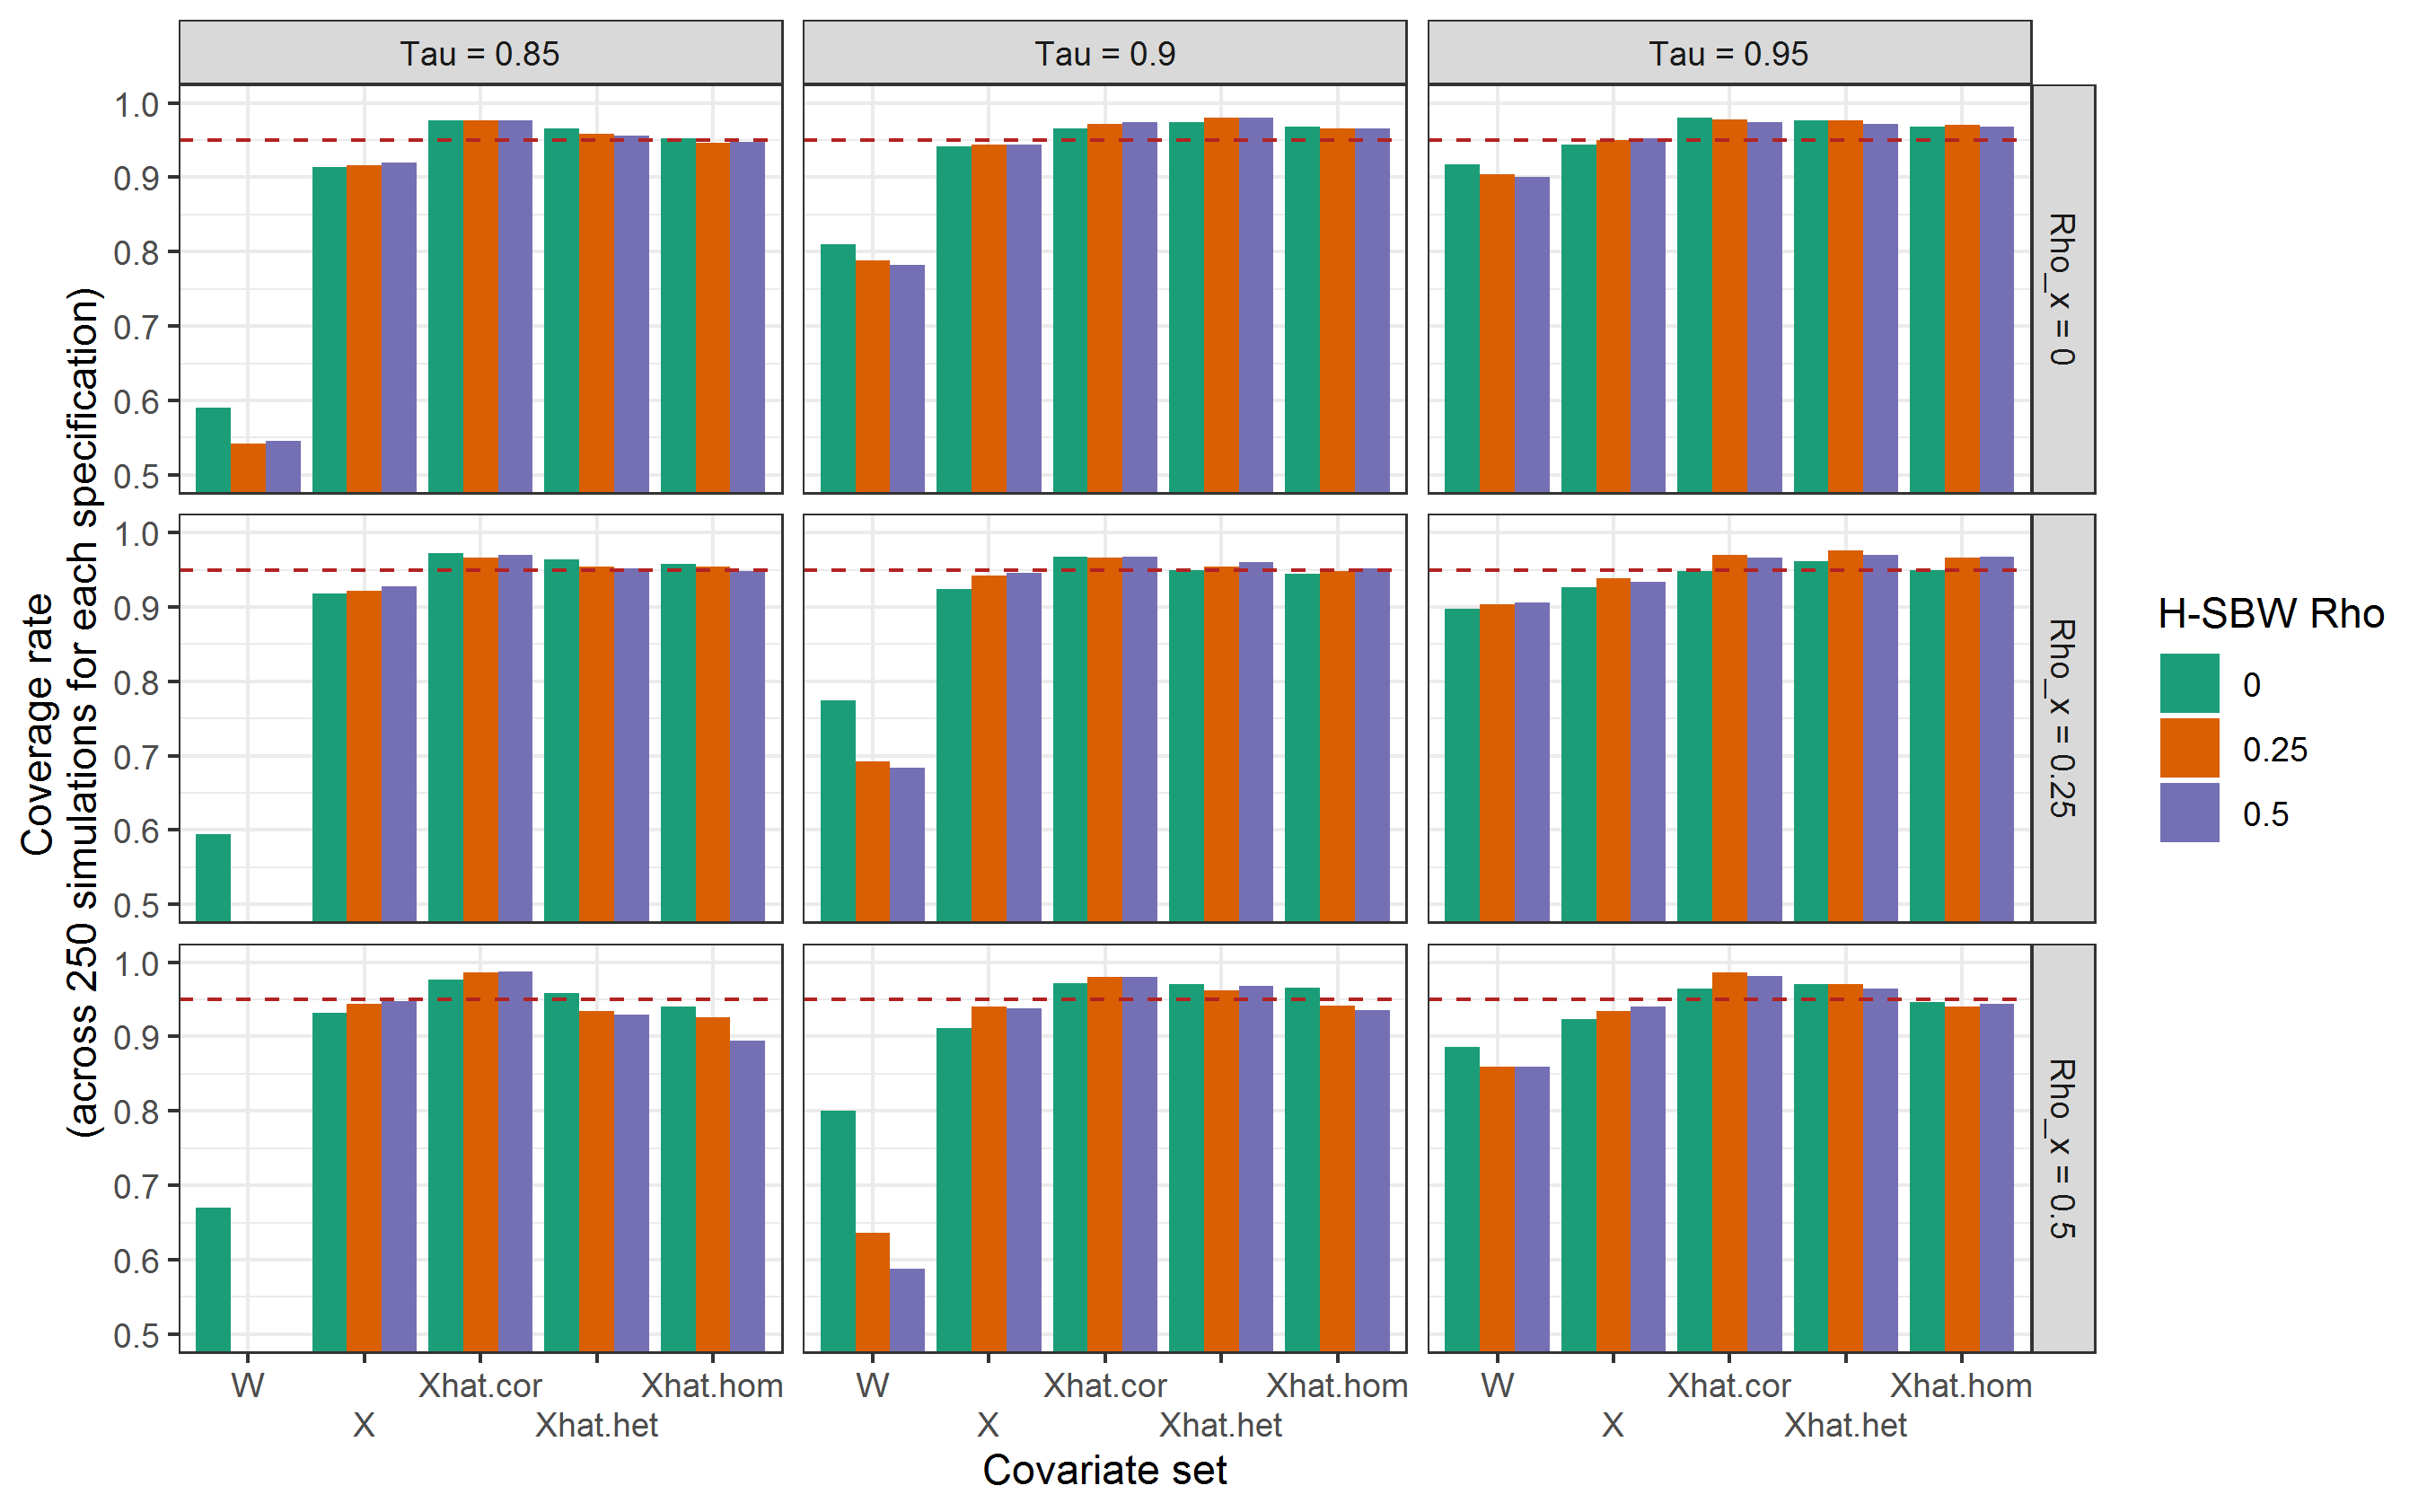
\includegraphics[scale=0.5]{01_Plots/coverage-plot-1.png}
    \subcaption{Averaged across 500 simulations for each specification}
\end{center}
\end{figure}

The figure displays one final and subtle but interesting feature: when we observe $X$, setting $\rho > 0$ appears to improve the coverage rates. We speculate this may be because H-SBW more evenly dispersing weights across states, increasing the ``effective sample size'' of the states, and thereby improving the asymptotic approximation of the variance estimates. We explore this feature more in Section~\ref{appssec:simstudyresults2} for different parameterizations of $\rho_y$. 

Finally, in Figure~\ref{fig:ciwdth} we evaluate the confidence interval lengths. As expected, we find that the H-SBW estimator is associated with lower lengths, reflecting that the estimators have decreased variability under our correlation structures. The optimal $\rho$ throughout is 0.25; however, we see that even $\rho = 0.5$ we obtain more precise inferences than when $\rho = 0$. Of course, in the context of measurement error, this also risks inducing more bias, though without measurement error this suggests benefits to using H-SBW even when our estimate of $\rho$ is a guess. All results are similar when considering homoskedastic measurement errors. 

\begin{figure}[H]\label{fig:ciwidth}
\begin{center}
    \caption{Confidence interval length}\label{fig:simcoverage2}
    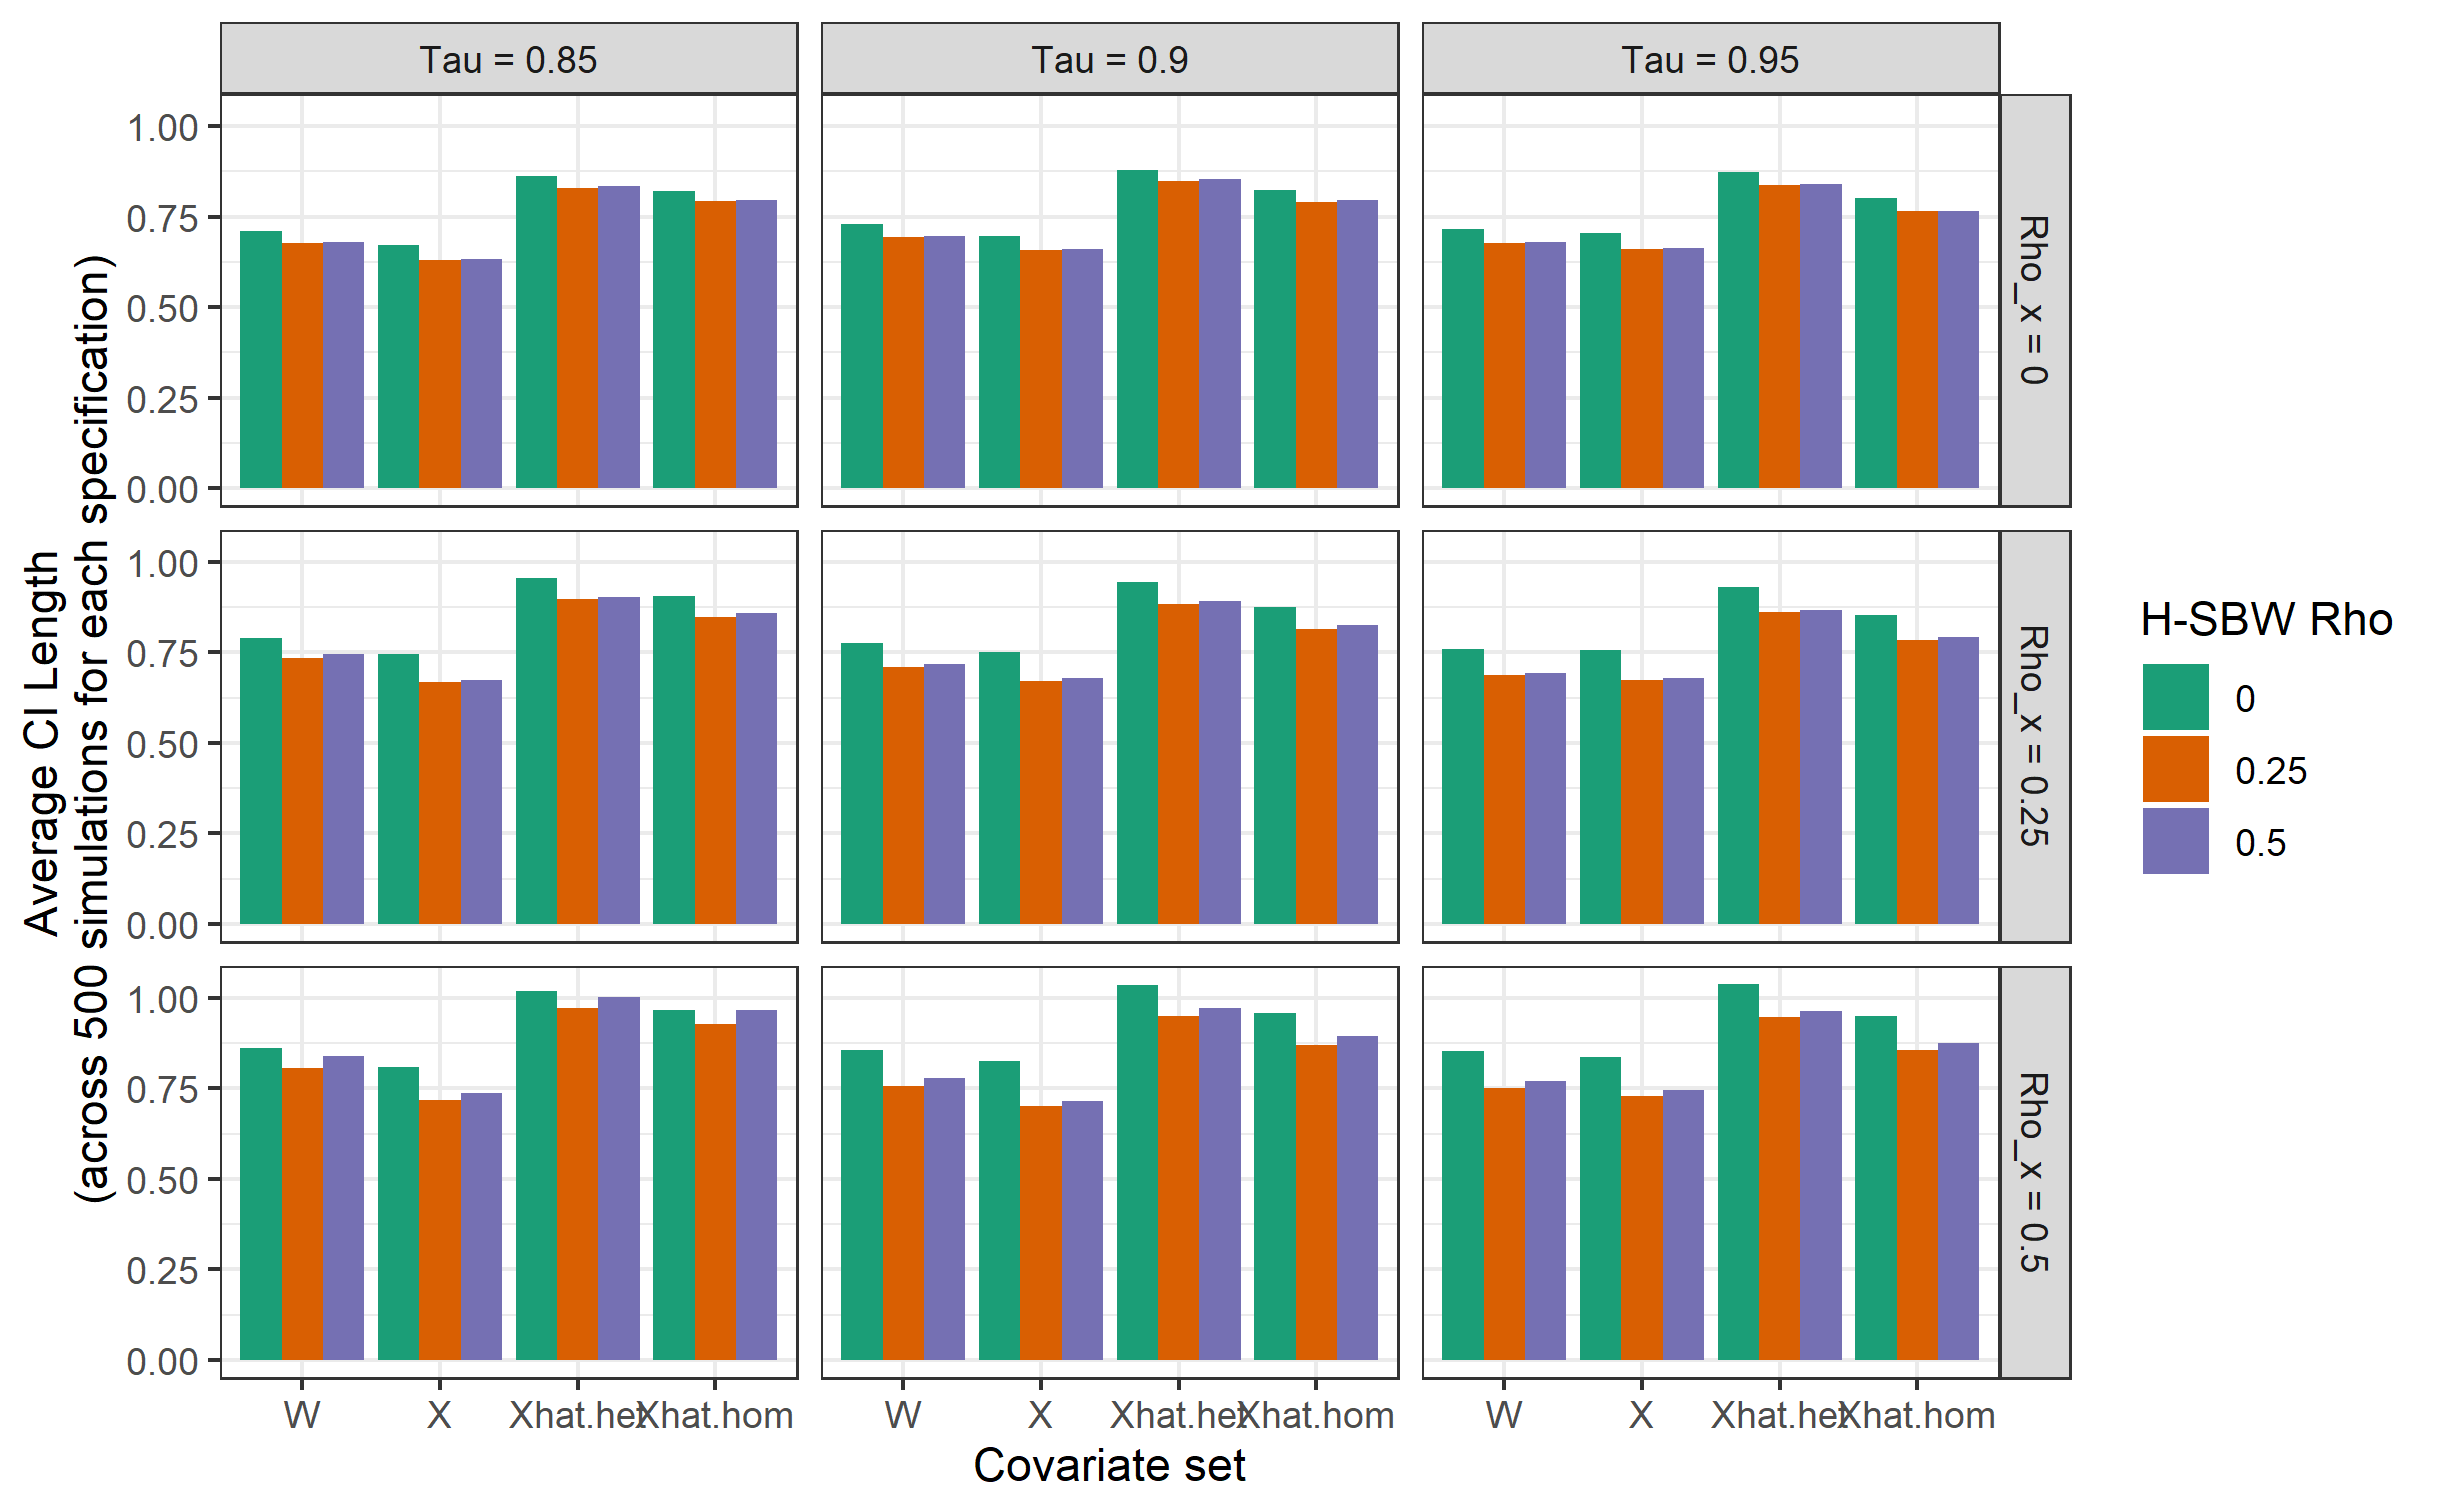
\includegraphics[scale=0.5]{01_Plots/ci-length-plot.png}
    \subcaption{Averaged across 500 simulations for each specification}
\end{center}
\end{figure}

We emphasize three takeaways from this simulation study. First, we do not find any evidence that the ``heterogeneous adjustment'' improves our estimates along any dimension, even in an ideal setting. However, this may in part reflect the distribution of sample sizes we generated, which we took to be uniform; perhaps with a different distribution these results would differ. Second, while setting $\rho > 0$ can increase the bias of our estimates in the context of measurement error, the bias is generally small relative to the bias of balancing on the noisy covariate measurements $W$. Even so, MSE improvements using H-SBW are still possible relative to SBW if we assume some non-negligible state-level random effect and relatively small measurement error. Third, accounting for the correlation in the data when using H-SBW and the data are measured with error may not be worth it given a small sample of states, despite the improved theoretic properties. This simulation study assumes throughout that we know the true data generating model for the outcome, and that are data are Gaussian. This study complements our validation study in Section~\ref{sec:results}, which has more direct bearing on understanding how these estimators might perform in our application.

\subsubsection{Additional results}\label{appssec:simstudyresults2}

In this subsection we demonstrate two additional results: first, that the correlated adjustment procedure proposed in Appendix~\ref{app:adjustmentdetails} is consistent as $m \to \infty$. Second, we consider confidence interval coverage for H-SBW with known covariates $X$, setting $m = 25$ but varying $\rho_y$, and demonstrate that H-SBW can improve the corresponding coverage rates relative to SBW when using the leave-one-state-out jackknife. 

\end{document}
